\documentclass[pdftex,12pt,a4paper]{article}
\usepackage{tabularx,tabulary,amsmath,amsfonts,amsthm,amssymb,latexsym}
\usepackage[pdftex]{graphicx}
% Exhibits awaiting regeneration on the 2026-Q2 production cut.
% To restore one: put the regenerated PNG in figures/ and change its
% \pendingexhibit call back to \includegraphics.
\newcommand{\pendingexhibit}[2][]{%
  \fbox{\begin{minipage}{0.88\linewidth}\centering\vspace{1.2em}%
  \textsf{\small Exhibit pending regeneration on the 2026-Q2 production cut}\\[0.4em]%
  \texttt{\footnotesize\detokenize{#2}}%
  \vspace{1.2em}\end{minipage}}}
\usepackage{float,xcolor,multirow,enumitem,colortbl,booktabs,adjustbox}
\usepackage{natbib}
\bibliographystyle{agsm}
\usepackage{caption}
\usepackage[figurename=Exhibit,tablename=Exhibit]{caption}
\usepackage{sectsty,titlecaps}
\usepackage{geometry}
\geometry{a4paper, total={165mm,235mm}, left=25mm, right=25mm, bottom=25mm, top=25mm}
\usepackage[hidelinks]{hyperref}
\begin{document}
	% ===== BEGIN section1_problem.tex =====
	% ======================================================================
	% FRONT MATTER + SECTION 1 — THE COMMITTEE'S PROBLEM
	% Drop-in for the R2 inverted structure. Template: cma_paper_v4.tex.
	% Data freeze: 2026-Q2 production cut, 18 assets, PE MSCI at w = 0.5.
	% Figures map from the exhibit build:
	%   figures/unintended_exposures.PNG <- exhibit_a3_unintended_exposures.png
	% Bootstrap-based intro numbers regenerated on the 2026-Q2 18-asset
	% freeze (run_bootstrap_q2.py, B=500): per-asset median residuals 30-115
	% bps, portfolio-level norm median 3.4%.
	% ======================================================================
	
	% ------------------------- FRONT MATTER -------------------------------
	
	\section*{Three Key Takeaways:}
	\begin{itemize}
		\item With the risk model, the benchmark, and the constraints held fixed, the CMA provider choice moves the Balanced-mandate expected return from $7.9\%$ (MATF) to $8.6\%$ (J.P. Morgan) to $11.3\%$ (BlackRock). The MATF-CMA framework gives the Investment Committee an auditable basis for that choice: every basis point of every CMA decomposes into a factor-implied return plus three declared adjustment channels.
		\item How much of the alternatives' historical excess return to admit as alpha is the single most consequential CMA decision. Scaling the admission from zero to the production policy lifts the claimed portfolio Sharpe ratio from $0.30$ to $0.35$ with almost no change in weights: mandate guardrails contain the allocation, and only the admission policy contains the claim. We propose two auditable caps for governing it.
		\item Consistency and uncertainty are quantified rather than asserted. The framework's deviation from the factor span reconciles exactly to its declared adjustments, against unattributable residuals of up to $5.5\%$ per asset under per-asset construction, and the factor structure with an economic prior halves the sampling bandwidth of the efficient frontier.
	\end{itemize}
	
	\begin{abstract}
		\noindent Capital market assumptions (CMAs) are the primary quantitative input to strategic asset allocation, yet allocation committees routinely adopt CMAs they cannot audit. Per-asset construction methods of the Grinold-Kroner type leave residuals outside the factor structure of the risk model, and the optimizer converts these unattributed residuals into factor bets that no committee has approved.
		
		\noindent We develop the MATF-CMA framework, in which each asset's expected return is the product of its loadings on nine tradable factors and market-implied factor risk premia, plus declared adjustments logged per asset: a regional valuation blend, an admitted historical alpha with weight $w_i \in [0,1]$, and a gross-of-fee add-on. The same loading matrix defines the covariance model, so the CMAs are alpha-beta consistent up to the declared adjustments, and the reconciliation is exact.
		
		\noindent We organize the empirical analysis around three committee decisions on a production 18-asset universe. The provider choice: on a common risk model, Balanced-mandate expected returns range from $7.9\%$ to $11.3\%$ across five CMA providers. The alpha admission: production admissions claim an idiosyncratic squared Sharpe ratio of $1.40$ against a factor opportunity set of $0.57$, and we propose two caps that turn the policy into pass-fail audit tests. The scenario choice: one vector of nine factor shocks reprices every asset, and the stress report separates factor repricing from the assumed survival of admitted skill. A bootstrap of 25 years of returns shows the factor structure halves the frontier's sampling bandwidth, equivalent to four times the sample.
	\end{abstract}
	
	\newpage
	
	% ------------------------- SECTION 1 ----------------------------------
	
	\sectionfont{\MakeUppercase}
	\section*{Capital Market Assumptions and Strategic Asset Allocation Using Multi-Asset Tradable Factors}\label{sec:intro}
	
	Capital market assumptions (CMAs) are long-term estimates of expected return, risk, and correlation for investable asset classes, and they are the primary quantitative input to strategic asset allocation (SAA). An allocation committee that signs off a CMA set is implicitly taking three decisions. It chooses whose expected returns to believe, it decides how much of the alternatives' historical excess return to treat as repeatable alpha, and it approves the scenarios under which the allocation will be stressed. The dominant production methodologies support none of these decisions auditably.
	
	The dominant methodologies build CMAs asset by asset. Grinold-Kroner-style decompositions \citep{GrinoldKroner2002} sum per-asset income, growth, and valuation components, and qualitative frameworks map assets to factor scores that are set by hand. Both approaches produce expected returns with no structural link to the covariance model used in the optimization, so the return vector generically lies outside the span of the risk model's factor loadings. The unattributed part is not harmless. The optimizer prices it as if it were alpha and converts it into factor bets that nobody approved. We measure both halves of this failure on a production 18-asset universe. Per-asset CMAs built from historical means leave unattributed residuals with per-asset medians of $30$ to $115$ basis points and a portfolio-level norm of $3.4\%$ across bootstrap draws. Point estimates reach $5.5\%$ on single assets. No diagnostic can trace these residuals to an intended assumption. A second weakness compounds the first. Per-asset point estimates inherit the noise of correlated component forecasts. We show by bootstrap that the resulting frontier bandwidth is roughly twice what a factor structure with an economic prior delivers.
	
	Exhibit~\ref{fig:unintended_exposures} shows the allocation consequence. We solve a long-only allocation at the benchmark volatility of $9.3\%$ twice, on the identical risk model, once under the MATF-CMAs of this paper and once under per-asset historical means. The historical-mean book claims an ex-ante excess Sharpe ratio of $0.92$ against $0.51$, runs an active FX exposure of $-0.22$ with broad tilts across Credit, Carry, Inflation, and Commodities, and carries $58\%$ of its active risk in idiosyncratic residuals. Under the constraints of a real mandate the two books converge in weights and still diverge in the claim. Unaudited CMAs damage the allocation where governance is light and damage the communicated numbers everywhere.
	
	\begin{figure}[H]
		\captionof{figure}{Unattributed Residuals Become Unintended Factor Bets}\label{fig:unintended_exposures}\vspace*{-0.5\baselineskip}
		\begin{center}
			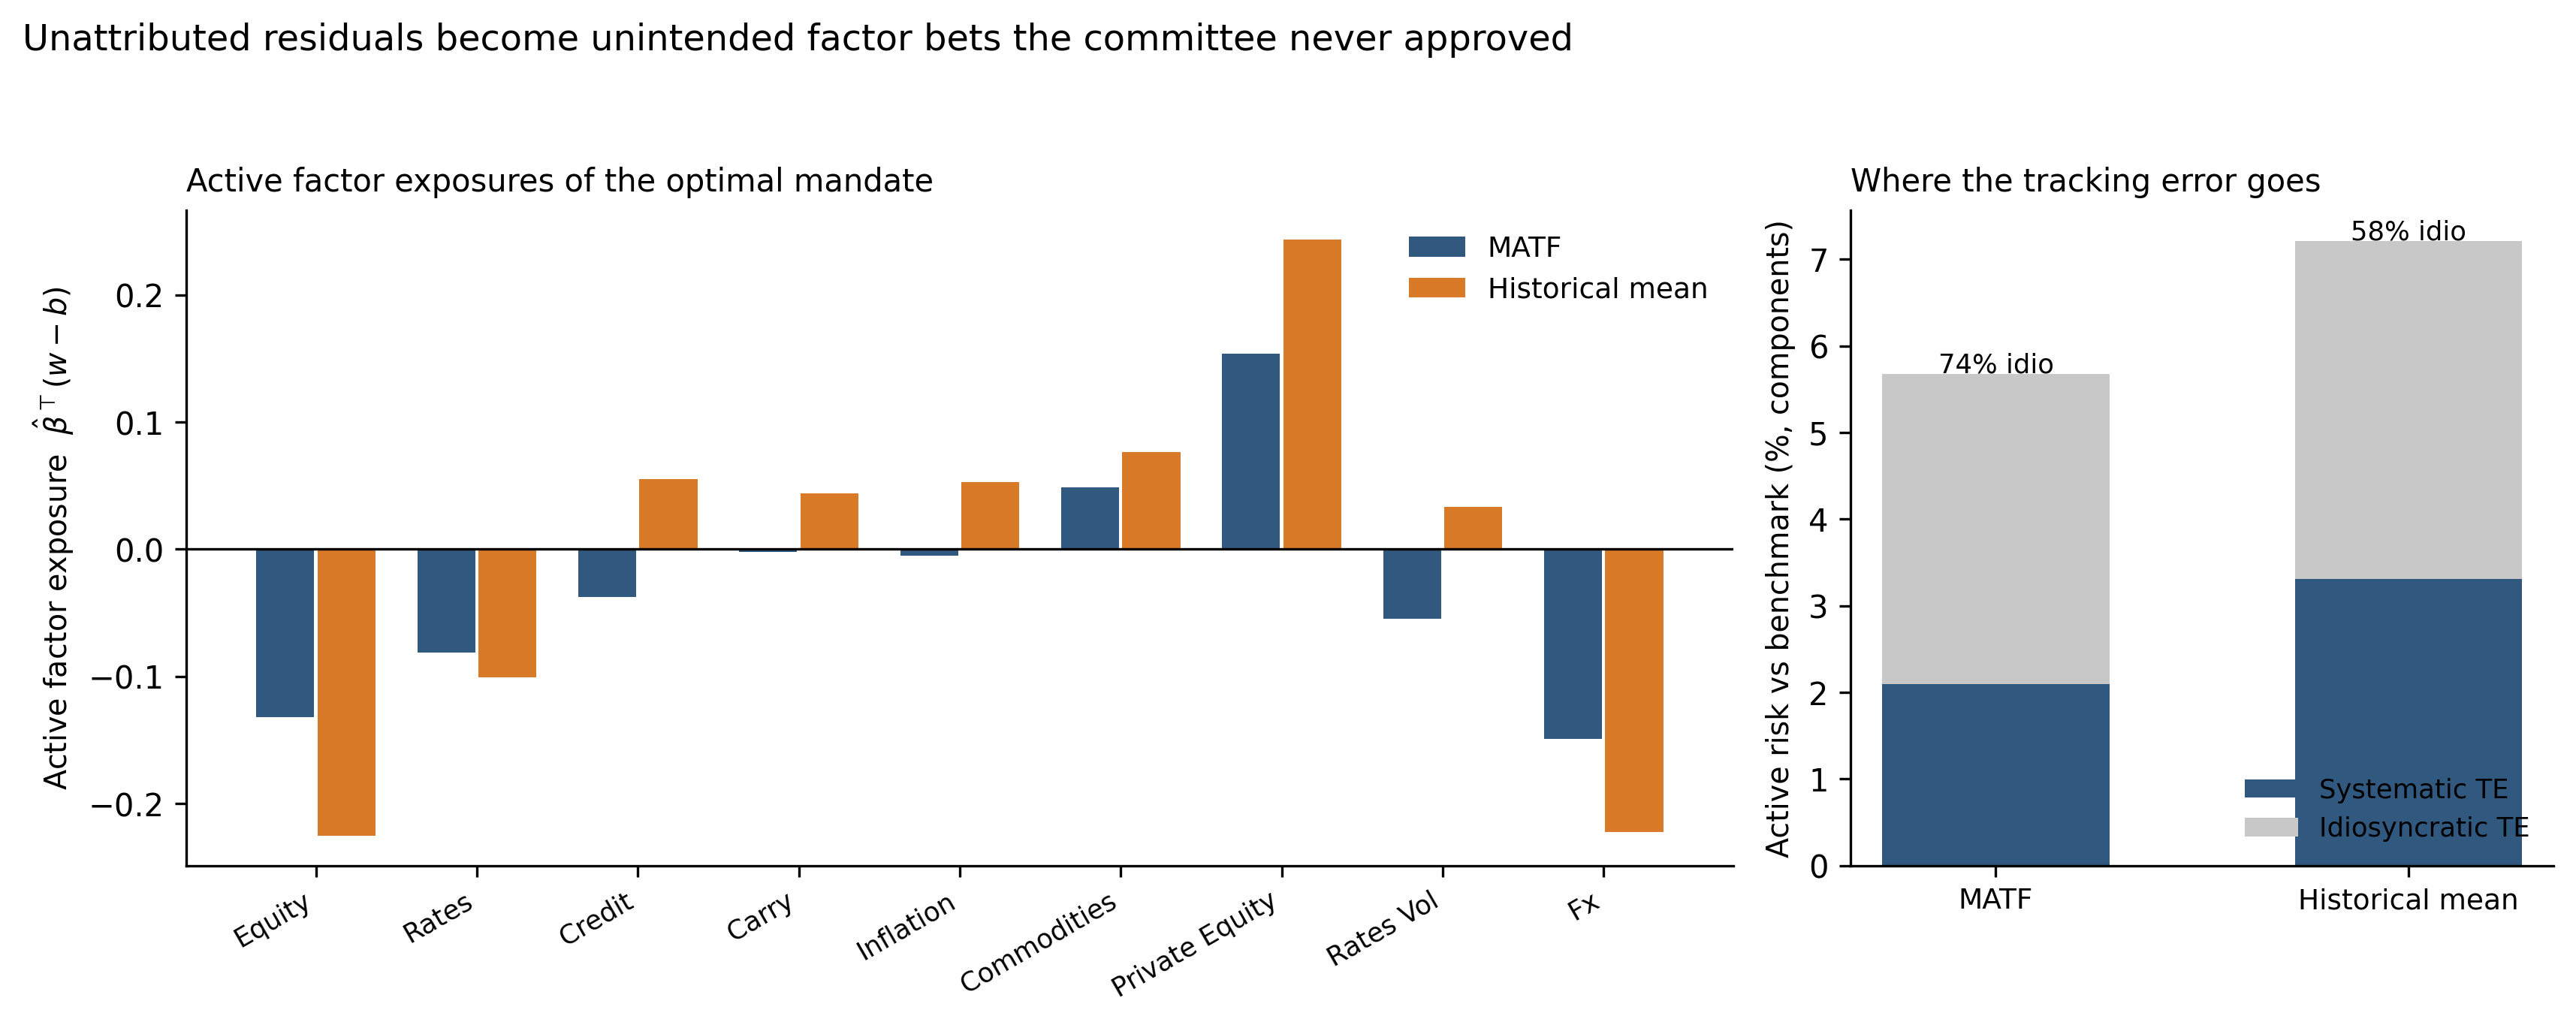
\includegraphics[width=0.95\linewidth]{figures/unintended_exposures.PNG}
		\end{center}
		\vspace*{-1.0\baselineskip}
		{\footnotesize Notes: long-only maximum-return allocations at the benchmark volatility target of $9.3\%$ on the identical MATF risk model, 2026-Q2 cut, USD. Left panel: active factor exposures $\hat{\boldsymbol\beta}^{\intercal}(\boldsymbol w - \boldsymbol b)$ of the optimal book against the Balanced benchmark under MATF-CMAs (blue) and per-asset historical-mean CMAs (orange). Right panel: decomposition of the active risk into systematic and idiosyncratic components.}
	\end{figure}
	
	This paper develops the MATF-CMA framework, which makes the three committee decisions explicit and auditable. The framework rests on two objects. The factor risk premia $\boldsymbol\lambda = (\lambda_1, \ldots, \lambda_M)^{\intercal}$ are expected excess returns of $M=9$ tradable factor portfolios, estimated from market-implied decompositions for the fundamental factors and from equilibrium Sharpe ratios for the structural factors. The factor loadings $\hat{\boldsymbol\beta}_i$ measure each asset's sensitivity to the factors, estimated by a sign-constrained clustered regression.\footnote{Throughout this paper, we use bold lowercase Greek for column vectors (e.g., $\boldsymbol\lambda$, $\boldsymbol\alpha$) and bold uppercase Greek or Roman for matrices (e.g., $\Sigma$, $\boldsymbol\beta$). Non-bold letters denote scalars. The superscript $\intercal$ denotes the transpose.} The asset-level CMA is
	\begin{equation}\label{eq:cma_i}
		\text{CMA}_i = r_f^{ref,3Y} + \hat{\boldsymbol\beta}_i^{\intercal} \boldsymbol\lambda + \text{declared adjustments}_i,
	\end{equation}
	where the declared adjustments of the next section are logged per asset and default to zero. The same loading matrix defines the risk model,
	\begin{equation}\label{eq:cma_ii}
		\Sigma = \boldsymbol\beta\, \Sigma_F\, \boldsymbol\beta^{\intercal} + D,
	\end{equation}
	with $\Sigma_F$ the $M \times M$ factor covariance matrix and $D$ the diagonal matrix of residual variances. Because Equations~\eqref{eq:cma_i} and~\eqref{eq:cma_ii} share $\hat{\boldsymbol\beta}$, the CMAs are alpha-beta consistent up to the declared adjustments, and the reconciliation between the two is exact rather than approximate.
	
	The structural guarantee distinguishes MATF-CMA from three related constructions. \cite{CeriaStubbsAlpha2013} achieve consistency procedurally through multi-stage factor-mimicking portfolios. \cite{BlackLitterman1992} guarantee spanning by reverse-optimizing from market-capitalization weights, which anchors expected returns to cap weights rather than to market observables. \cite{RoncalliXu2024} prove a zero residual premium for the tangency portfolio in a factor reformulation, again with cap-weight-derived premia. MATF-CMA obtains the guarantee by construction from market-observable premia, and it extends the guarantee to a governed exception. Deviations from the factor span are permitted only through the declared channels, so the committee sees every exception it grants.
	
	The MATF-CMA framework complements the ROSAA tactical allocation framework of \citet{Rosaa2026}. ROSAA optimizes multi-fund active portfolios against a risk-budgeted SAA benchmark using short-horizon tactical alphas. MATF-CMA constructs the long-horizon strategic $\boldsymbol\mu$ that anchors that benchmark, so the two layers stack.
	
	The paper is organized around the three decisions. The next section presents the framework at the level the committee signs off, with the estimation development in Appendices~C and~D. Section ``Decision One: The Provider Choice'' compares five CMA providers on a common risk model. Section ``Decision Two: The Alpha Admission'' prices the admission policy and proposes two governance caps. Section ``Decision Three: Coherent Scenarios'' defines scenarios as factor-shock vectors and separates factor repricing from assumed skill. Section ``How Much to Trust the Numbers'' quantifies estimation uncertainty and verifies the consistency reconciliation. Section ``Implications for Practice'' summarizes the operational consequences for institutional SAA processes.
	
	% ===== END section1_problem.tex =====
	
	% ===== BEGIN section2_framework.tex =====
	% ======================================================================
	% SECTION 2 — THE MATF-CMA FRAMEWORK IN TWO EXHIBITS
	% Drop-in for the R2 inverted structure. Template: cma_paper_v4.tex.
	% Data freeze: 2026-Q2 production cut. Nine-factor table values computed
	% from the frozen workbook (factor_excess_cma, x_covar diagonals).
	% Figures map from the exhibit build:
	%   figures/construction_waterfall.PNG <- exhibit_a1_construction_waterfall.png
	% Bib note: the loading estimator is cited to Rosaa2026; the dedicated
	% methodology papers (CSDA/JSS) are cited once they carry a citable form.
	% ======================================================================
	
	\sectionfont{\MakeUppercase}
	\section*{The MATF-CMA Framework}\label{sec:framework}
	
	This section presents the framework at the level the Investment Committee signs off: nine factors with their premia, one loading matrix shared with the risk model, and three declared adjustment channels. The estimation development sits in Appendix~C for the factor premia and Appendix~D for the loadings and the multi-currency construction.
	
	\subsection*{Nine Tradable Factors and Their Premia}\label{subsec:factors}
	
	The MATF specification uses nine tradable factors, each implemented as an investable, volatility-targeted portfolio of futures or index trackers.\footnote{We apply the MATF model of \cite{Rosaa2026} with two additions, a rates-volatility factor and a risk-only FX factor. Volatility targets are differentiated by asset class: $15\%$ for Equity and Commodities, $7\%$ for Private Equity and FX, $6\%$ for Rates, and $5\%$ for the remaining factors. Rescaling a factor rescales its betas inversely and leaves CMAs, covariances, and optimization outputs unchanged.} Tradability is the discipline of the framework: every premium is the expected excess return of a portfolio the desk could hold, not a score.
	
	Exhibit~\ref{tab:nine_factors} lists the factors, the source of each premium, and the current values on the production cut. The premia divide into two groups. The fundamental factors carry market-implied premia. The Equity premium comes from the payout- and cyclically-adjusted earnings yield (P-CAEY) of \citet{HaghaniWhite2024}, blended per region as described below. The Rates premium combines the OIS-implied term premium with the roll-down carry of the curve, and the Credit premium is the CDS spread net of the actuarial expected loss \citep{Ilmanen2011}. The structural factors, for which no market yield provides a clean decomposition, carry equilibrium premia set as a long-run Sharpe ratio times the factor's volatility target. The rates-volatility factor prices the short-volatility exposure embedded in all corporate assets \citep{Morris2026}, and the FX factor carries a zero premium by an equilibrium argument: the dollar level is uncompensated, while the compensated currency premium is already in the Carry factor \citep{LustigRV2011}. The FX factor therefore contributes to the risk model and not to expected returns.
	
	\begin{table}[H]
		\captionof{table}{Nine Tradable Factors: Premium Source and Current Values}\label{tab:nine_factors}\vspace*{-0.5\baselineskip}
		\begin{center}
			\footnotesize
			\begin{tabular}{l l rrr}
				\toprule
				\textbf{Factor} & \textbf{Premium source} & \textbf{Premium} & \textbf{Vol} & \textbf{Premium/Vol} \\
				& & (\%) & (\%) & \\
				\midrule
				Equity      & P-CAEY earnings yield, regional blend        & 3.61 & 15.4 & 0.23 \\
				Rates       & OIS term premium + curve roll-down           & 1.31 & 5.6  & 0.23 \\
				Credit      & CDS spread net of expected loss              & 1.42 & 4.7  & 0.30 \\
				Carry       & Equilibrium Sharpe prior                     & 1.25 & 4.5  & 0.28 \\
				Inflation   & Equilibrium Sharpe prior                     & 0.75 & 4.7  & 0.16 \\
				Commodities & Equilibrium Sharpe prior                     & 2.25 & 16.0 & 0.14 \\
				Private Equity & Equilibrium Sharpe prior                  & 3.50 & 7.1  & 0.49 \\
				Rates Vol   & Equilibrium Sharpe prior on swaption carry   & 1.25 & 5.2  & 0.24 \\
				FX          & Zero by equilibrium (risk-only factor)       & 0.00 & 6.9  & 0.00 \\
				\bottomrule
			\end{tabular}
		\end{center}
		\vspace*{-0.5\baselineskip}
		{\footnotesize Notes: 2026-Q2 production cut, USD. Premium is the base excess CMA $\lambda_j$ of the factor portfolio, and Vol is the annualized factor volatility from the production factor covariance. Premium/Vol is their ratio. Appendix~C derives each premium.}
	\end{table}
	
	\subsection*{One Loading Matrix, Shared with the Risk Model}\label{subsec:loadings}
	
	The factor loadings $\hat{\boldsymbol\beta}$ are estimated once per production cut from a regression of asset excess returns on factor excess returns, with two economic disciplines. First, loadings carry sign constraints that encode economic priors, as summarized in Exhibit~\ref{tab:sign_constraints}: core risk premia enter non-negatively for long-only assets, the rates-volatility loading is non-positive because corporate assets are implicitly short rates volatility, and the Private Equity factor is reserved for private-market assets. Second, a clustering-based regularization stabilizes the loadings of correlated factors and correlated assets. The estimator and its properties are developed in \citet{Rosaa2026} and the companion methodology papers, and Appendix~D states the configuration used in production.\footnote{The estimator is available in the open-source \texttt{factorlasso} package. The replication repository of this paper pins the version used for the frozen cut.}
	
	The same matrix $\hat{\boldsymbol\beta}$ defines the covariance model of Equation~\eqref{eq:cma_ii}. The shared loadings are the consistency mechanism of the framework, and the diagnostic of Appendix~A measures any CMA vector against this risk model, whether produced by MATF or by an external provider.
	
	\begin{table}[H]
		\captionof{table}{Sign Constraints Encode the Economic Priors of the Loading Matrix}\label{tab:sign_constraints}\vspace*{-1.0\baselineskip}
		\begin{center}
			\begin{adjustbox}{max width=\textwidth}
				\begin{tabular}{l*{9}{c}}
					\toprule
					\textbf{Asset class} & \textbf{Equity} & \textbf{Rates} & \textbf{Credit} & \textbf{Carry} & \textbf{Inflation} & \textbf{Commod.} & \textbf{PE} & \textbf{Rates Vol} & \textbf{FX} \\
					\midrule
					Fixed Income & $\geq 0$ & $\geq 0$ & $\geq 0$ & $\geq 0$ & -- & -- & $= 0$ & $\leq 0$ & -- \\
					Equity & $\geq 0$ & $\geq 0$ & $\geq 0$ & $\geq 0$ & -- & -- & $= 0$ & $\leq 0$ & -- \\
					PE / PD / Diversified & $\geq 0$ & $\geq 0$ & $\geq 0$ & $\geq 0$ & -- & -- & $\geq 0$ & $\leq 0$ & -- \\
					Other (HF, Real Assets) & -- & -- & -- & -- & -- & -- & $= 0$ & -- & -- \\
					\bottomrule
				\end{tabular}
			\end{adjustbox}
		\end{center}
		\small
		NOTE: ``$\geq 0$'' = non-negative; ``$\leq 0$'' = non-positive; ``$= 0$'' = forced zero; ``--'' = unconstrained.
	\end{table}
	
	\subsection*{Asset-Level CMAs and the Three Declared Channels}\label{subsec:asset_cmas}
	
	The framework operates natively in excess return space. The factor-implied expected excess return of asset $i$ in reference currency $ref$ is
	\begin{equation}\label{eq:cma1}
		\text{CMA}_i^{(ref),factor} = \hat{\boldsymbol\beta}_i^{(ref)\intercal} \boldsymbol\lambda = \sum_{j=1}^{M} \hat{\beta}_{ij}^{(ref)} \cdot \lambda_j .
	\end{equation}
	The published excess CMA adds three declared adjustment channels:
	\begin{equation}\label{eq:cma2a}
		\text{CMA}_i^{(ref),excess} = \text{CMA}_i^{(ref),factor} + b_i + w_i \cdot \alpha_i^{(ref)} + a_i .
	\end{equation}
	The regional valuation blend $b_i$ applies to benchmark equity and government sleeves, where the regional market-implied premium of Appendix~C differs from the global factor-implied value. The admitted historical alpha $w_i \cdot \alpha_i$ applies to selected alternatives, where $\alpha_i$ is the Jensen alpha recovered as the average regression residual,
	\begin{equation}\label{eq:jensen}
		\alpha^{(ref)}_i = \bar{Y}^{(ref)}_i - \hat{\boldsymbol\beta}^{(ref)\intercal}_i \bar{\boldsymbol X},
	\end{equation}
	and $w_i \in [0,1]$ is the admission weight set by the committee, governed in Section ``Decision Two: The Alpha Admission''. The gross add-on $a_i$ converts selected fund CMAs to a gross-of-fee basis where required for reporting. Equities and bonds carry $w_i = 0$, so their consistency with the factor model is exact up to the blend. The total CMA adds the reference-currency risk-free rate,
	\begin{equation}\label{eq:cma2}
		\text{CMA}_i^{(ref)} = r_f^{ref,3Y} + \text{CMA}_i^{(ref),excess},
	\end{equation}
	where the 3-year government yield aligns with the CMA horizon and carries minimal term-premium contamination \citep{ACM2013}. The multi-currency construction holds $\boldsymbol\lambda$ identical across reference currencies and re-estimates loadings against reference-currency returns, with the details and a worked example in Appendix~D.
	
	Exhibit~\ref{fig:construction_waterfall} shows the construction for the full 18-asset universe of this paper. Every basis point of every excess CMA is one of four colors: factor-implied, blend, admitted alpha, or add-on. The four components sum to the published number exactly, and the replication code asserts the identity on the workbook at each production cut. The waterfall is the audit artifact of the framework: the committee that approves it has seen every deviation from the factor model it is granting. The remaining sections put that property to work.
	
	\begin{figure}[H]
		\captionof{figure}{Every Excess CMA Decomposes into Declared Channels: Nothing Is Unattributed}\label{fig:construction_waterfall}\vspace*{-0.5\baselineskip}
		\begin{center}
			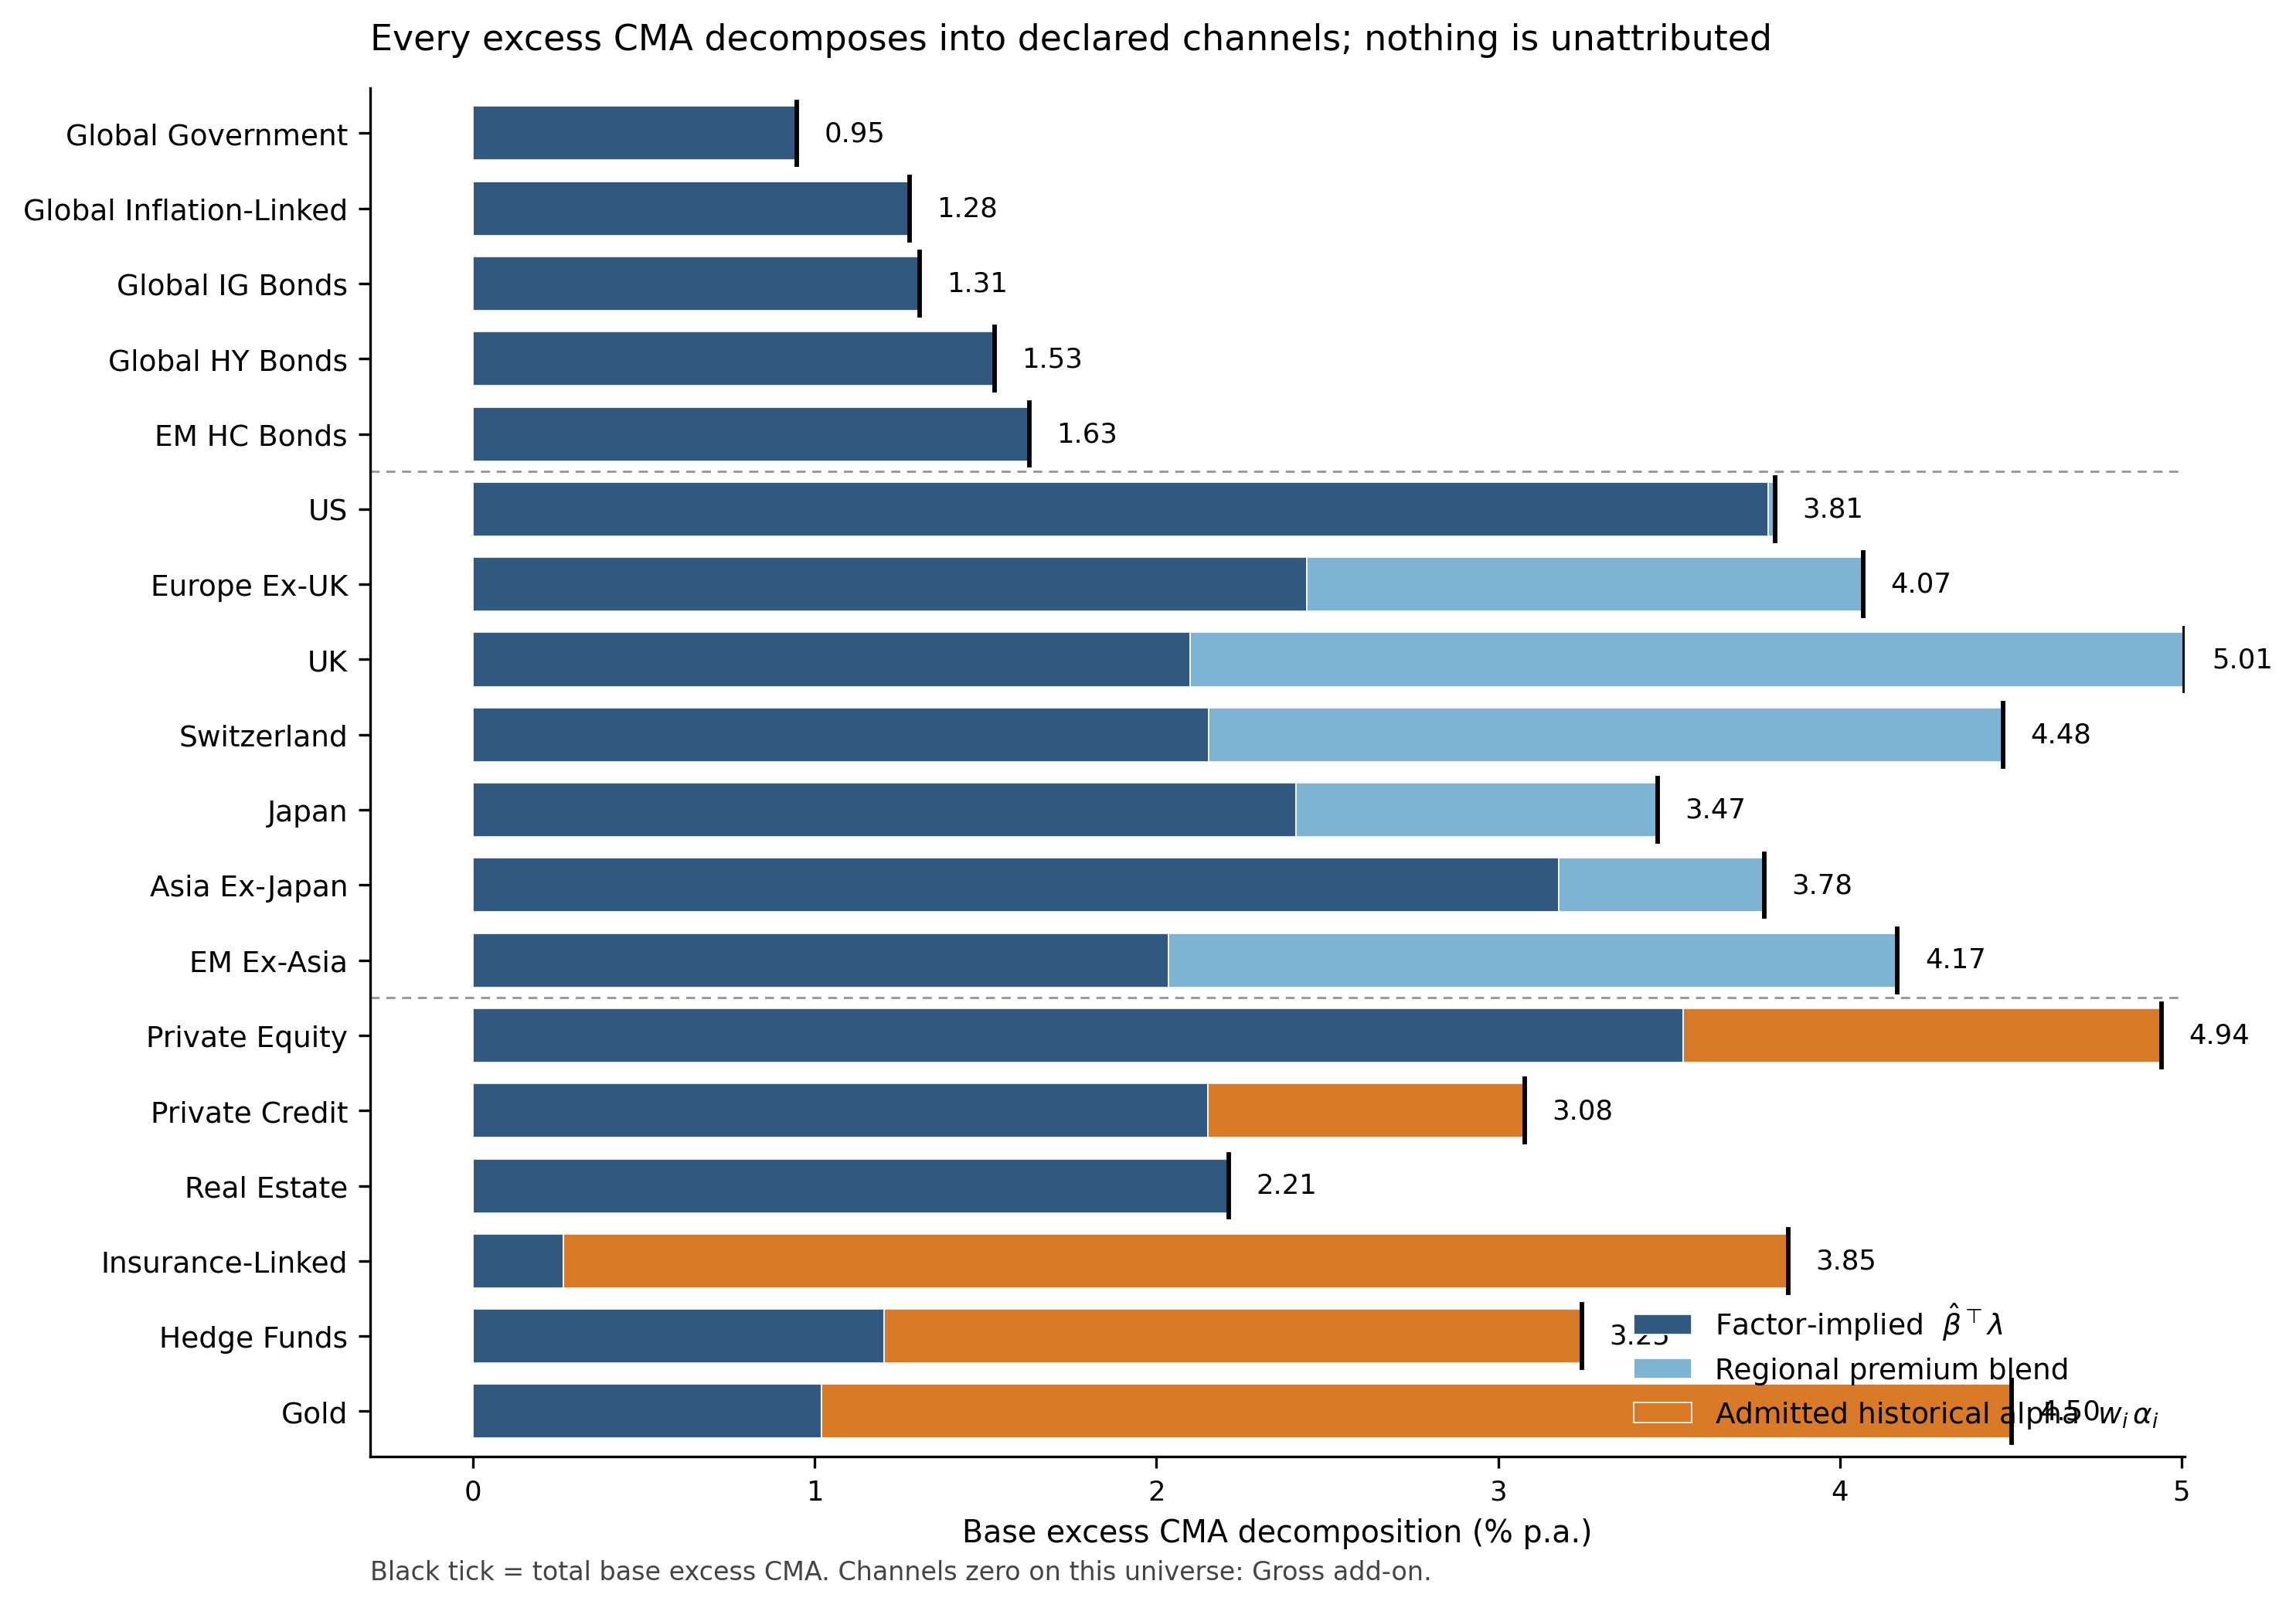
\includegraphics[width=0.9\linewidth]{figures/construction_waterfall.PNG}
		\end{center}
		\vspace*{-1.0\baselineskip}
		{\footnotesize Notes: 2026-Q2 production cut, USD, base excess CMAs in percent per annum. Stacked components per Equation~\eqref{eq:cma2a}: factor-implied $\hat{\boldsymbol\beta}^{\intercal}\boldsymbol\lambda$, regional valuation blend, admitted historical alpha $w_i \alpha_i$, and gross add-on. The black tick marks the published excess CMA. The add-on channel is zero on this universe.}
	\end{figure}
	
	% ===== END section2_framework.tex =====
	
	% ===== BEGIN section3_provider.tex =====
	% ======================================================================
	% SECTION 3 — DECISION ONE: THE PROVIDER CHOICE
	% Drop-in for the R2 inverted structure. Template: cma_paper_v4.tex.
	% Data freeze: 2026-Q2 production cut, 18 assets, PE MSCI at w = 0.5.
	% All table values from exhibit_b45_peer_frontier.py on the frozen cut.
	% Figures map from the exhibit build:
	%   figures/provider_frontier_with_alts.PNG <- exhibit_b5_frontier_with_alts.png
	% The w/o-Alts family (frontier + the Government 10.9%-15.8% bond
	% rotation) goes to Appendix F per the signed-off outline.
	% Bib entries required:
	%   HorizonSurvey2025 [TODO: confirm entry] Horizon Actuarial Services.
	%     2025. Survey of Capital Market Assumptions.
	% ======================================================================
	
	\sectionfont{\MakeUppercase}
	\section*{Decision One: The Provider Choice}\label{sec:provider}
	
	Allocation committees choose a CMA provider before they choose an allocation, and the choice is rarely priced. We price it directly. We optimize the same mandates, on the same benchmark, under the same constraints, on the same risk model, and change only the expected returns: the MATF-CMAs of this paper against the published sets of J.P. Morgan, BlackRock, UBS, and LGT Capital Partners.\footnote{All provider returns are arithmetic total returns for a USD investor. Native-currency lines convert by uncovered interest parity with each provider's own cash rates. Sleeves without a published provider line are held at the MATF value and carry no cross-provider tilt by construction: Switzerland, Real Estate, Insurance-Linked, and Gold for J.P. Morgan and BlackRock, additionally the UK for UBS and LGT Capital Partners. J.P. Morgan publishes no CHF assumption block.} Holding the risk model fixed is a deliberate simplification. It isolates the return disagreement and understates any disagreement in the providers' risk views, and we accept the trade-off because asset-level provider covariances are not published in comparable form.
	
	Exhibit~\ref{tab:provider_saa} reports the Balanced-with-Alternatives solution per provider. The headline is the top row of Panel~B. On an identical risk model with an identical $10.5\%$ volatility book, the expected total return runs from $7.9\%$ under MATF to $8.2\%$ under LGT Capital Partners, $8.6\%$ under J.P. Morgan, $8.7\%$ under UBS, and $11.3\%$ under BlackRock. The implied excess Sharpe ratio runs from $0.35$ to $0.67$. Nothing in the portfolios justifies the spread, because the portfolios are nearly the same book. The spread is a pure disagreement about expected returns, and the committee that adopts a provider adopts it.
	
	\begin{table}[H]
		\captionof{table}{The Provider Choice Priced: Balanced Mandate on a Common Risk Model, Benchmark, and Constraints}\label{tab:provider_saa}\vspace*{-0.5\baselineskip}
		\begin{center}
			\footnotesize
			\begin{tabular}{l rrrrrr}
				\toprule
				& \textbf{Bench} & \textbf{MATF} & \textbf{JPM} & \textbf{BR} & \textbf{UBS} & \textbf{CP} \\
				\midrule
				\multicolumn{7}{l}{\textit{Panel A: optimal weights (\%)}} \\
				Fixed income (5 sleeves)  & 28.0 & 14.0 & 14.0 & 14.0 & 14.0 & 14.0 \\
				US                        & 28.7 & 31.8 & 30.4 & 35.1 & 27.0 & 24.0 \\
				Europe ex-UK              & 3.7  & 5.6  & 5.6  & 5.6  & 5.6  & 5.6 \\
				UK                        & 1.3  & 2.0  & 0.7  & 0.7  & 2.0  & 2.0 \\
				Switzerland               & 0.8  & 1.3  & 1.3  & 0.4  & 1.3  & 1.3 \\
				Japan                     & 2.0  & 1.0  & 1.0  & 1.8  & 3.1  & 3.1 \\
				Asia ex-Japan             & 0.9  & 0.4  & 1.3  & 0.4  & 1.3  & 1.3 \\
				EM ex-Asia                & 4.5  & 6.8  & 6.8  & 2.3  & 6.8  & 6.8 \\
				Private Equity            & 15.0 & 22.5 & 22.5 & 22.5 & 22.5 & 22.5 \\
				Private Credit            & 3.0  & 1.5  & 4.5  & 4.5  & 4.5  & 4.5 \\
				Real Estate               & 3.0  & 1.5  & 1.5  & 1.5  & 1.5  & 1.5 \\
				Insurance-Linked          & 3.0  & 4.5  & 4.5  & 2.2  & 4.5  & 4.5 \\
				Hedge Funds               & 3.0  & 2.7  & 1.5  & 4.5  & 1.5  & 4.5 \\
				Gold                      & 3.0  & 4.5  & 4.5  & 4.5  & 4.5  & 4.5 \\
				\midrule
				\multicolumn{7}{l}{\textit{Panel B: portfolio statistics}} \\
				Expected total return (\%) &      & 7.92 & 8.57 & 11.26 & 8.66 & 8.15 \\
				Volatility (\%)            &      & 10.6 & 10.4 & 10.5  & 10.4 & 10.1 \\
				Excess Sharpe ratio        &      & 0.35 & 0.42 & 0.67  & 0.43 & 0.39 \\
				Tracking error (\%)        &      & 1.50 & 1.41 & 1.50  & 1.36 & 1.19 \\
				\bottomrule
			\end{tabular}
		\end{center}
		\vspace*{-0.5\baselineskip}
		{\footnotesize Notes: Balanced with Alternatives mandate, 2026-Q2 cut, USD. Each column maximizes the provider's expected return on the common MATF risk model with weights within $\pm 50\%$ of the benchmark and tracking error capped at $1.5\%$. Expected returns are arithmetic total, and the excess Sharpe ratio nets the $4.2\%$ reference risk-free rate. Held sleeves per provider are listed in the text footnote.}
	\end{table}
	
	The weights tell the committee where the disagreement lives. Every provider funds the same trade at this tracking-error budget: all five cut every bond sleeve to its floor, and they disagree only about where the proceeds go. Within equities, the US weight runs from $24.0\%$ under LGT Capital Partners to $35.1\%$ under BlackRock, and BlackRock alone cuts EM ex-Asia to its floor while the others hold it at the cap. Within alternatives, Private Credit separates MATF at the floor from everyone else at the cap. Hedge Funds separate BlackRock and LGT Capital Partners at the cap from J.P. Morgan and UBS at the floor, and BlackRock alone cuts Insurance-Linked. One row is provider-invariant: Private Equity sits at its $22.5\%$ cap in every column. Every provider's private-equity assumption saturates the constraint, so the PE weight is set by the box and not by the CMA. The next section shows that the PE assumption still matters, because it moves the claimed return of the book.
	
	Exhibit~\ref{fig:provider_frontier} places the five providers on the mandate frontier and adds the MATF scenario band of Section ``Decision Three''. Two facts stand out. The mainstream providers cluster inside the band: the gap between MATF and J.P. Morgan or UBS is $0.65$ to $0.74\%$ on the Balanced mandate, which is small against the $5.2\%$ width of the 2022-stress to 2023-upside range. BlackRock does not: its Balanced expectation of $11.3\%$ exceeds even the 2023-upside repricing of the MATF book at $9.7\%$, so the BlackRock base case sits beyond the framework's upside scenario. The MATF numbers sit at the conservative end of the mainstream cluster, and the placement is quantifiable against the 41-advisor survey of \citet{HorizonSurvey2025}. On a 10-year geometric basis, every traditional MATF sleeve sits at or below the survey median, with US equity at the median and the emerging-market and high-yield sleeves below the 25th percentile.\footnote{We compare the geometric approximation of each MATF total CMA (arithmetic total minus one half the variance) against the survey's geometric 10-year distributions. The 2025 survey aggregates assumption sets effective around January 2025, one vintage behind the provider sets of Exhibit~\ref{tab:provider_saa}. Horizon publishes a new edition each summer.}
	
	\begin{figure}[H]
		\captionof{figure}{Provider Frontiers on the Common Risk Model with the MATF Scenario Band}\label{fig:provider_frontier}\vspace*{-0.5\baselineskip}
		\begin{center}
			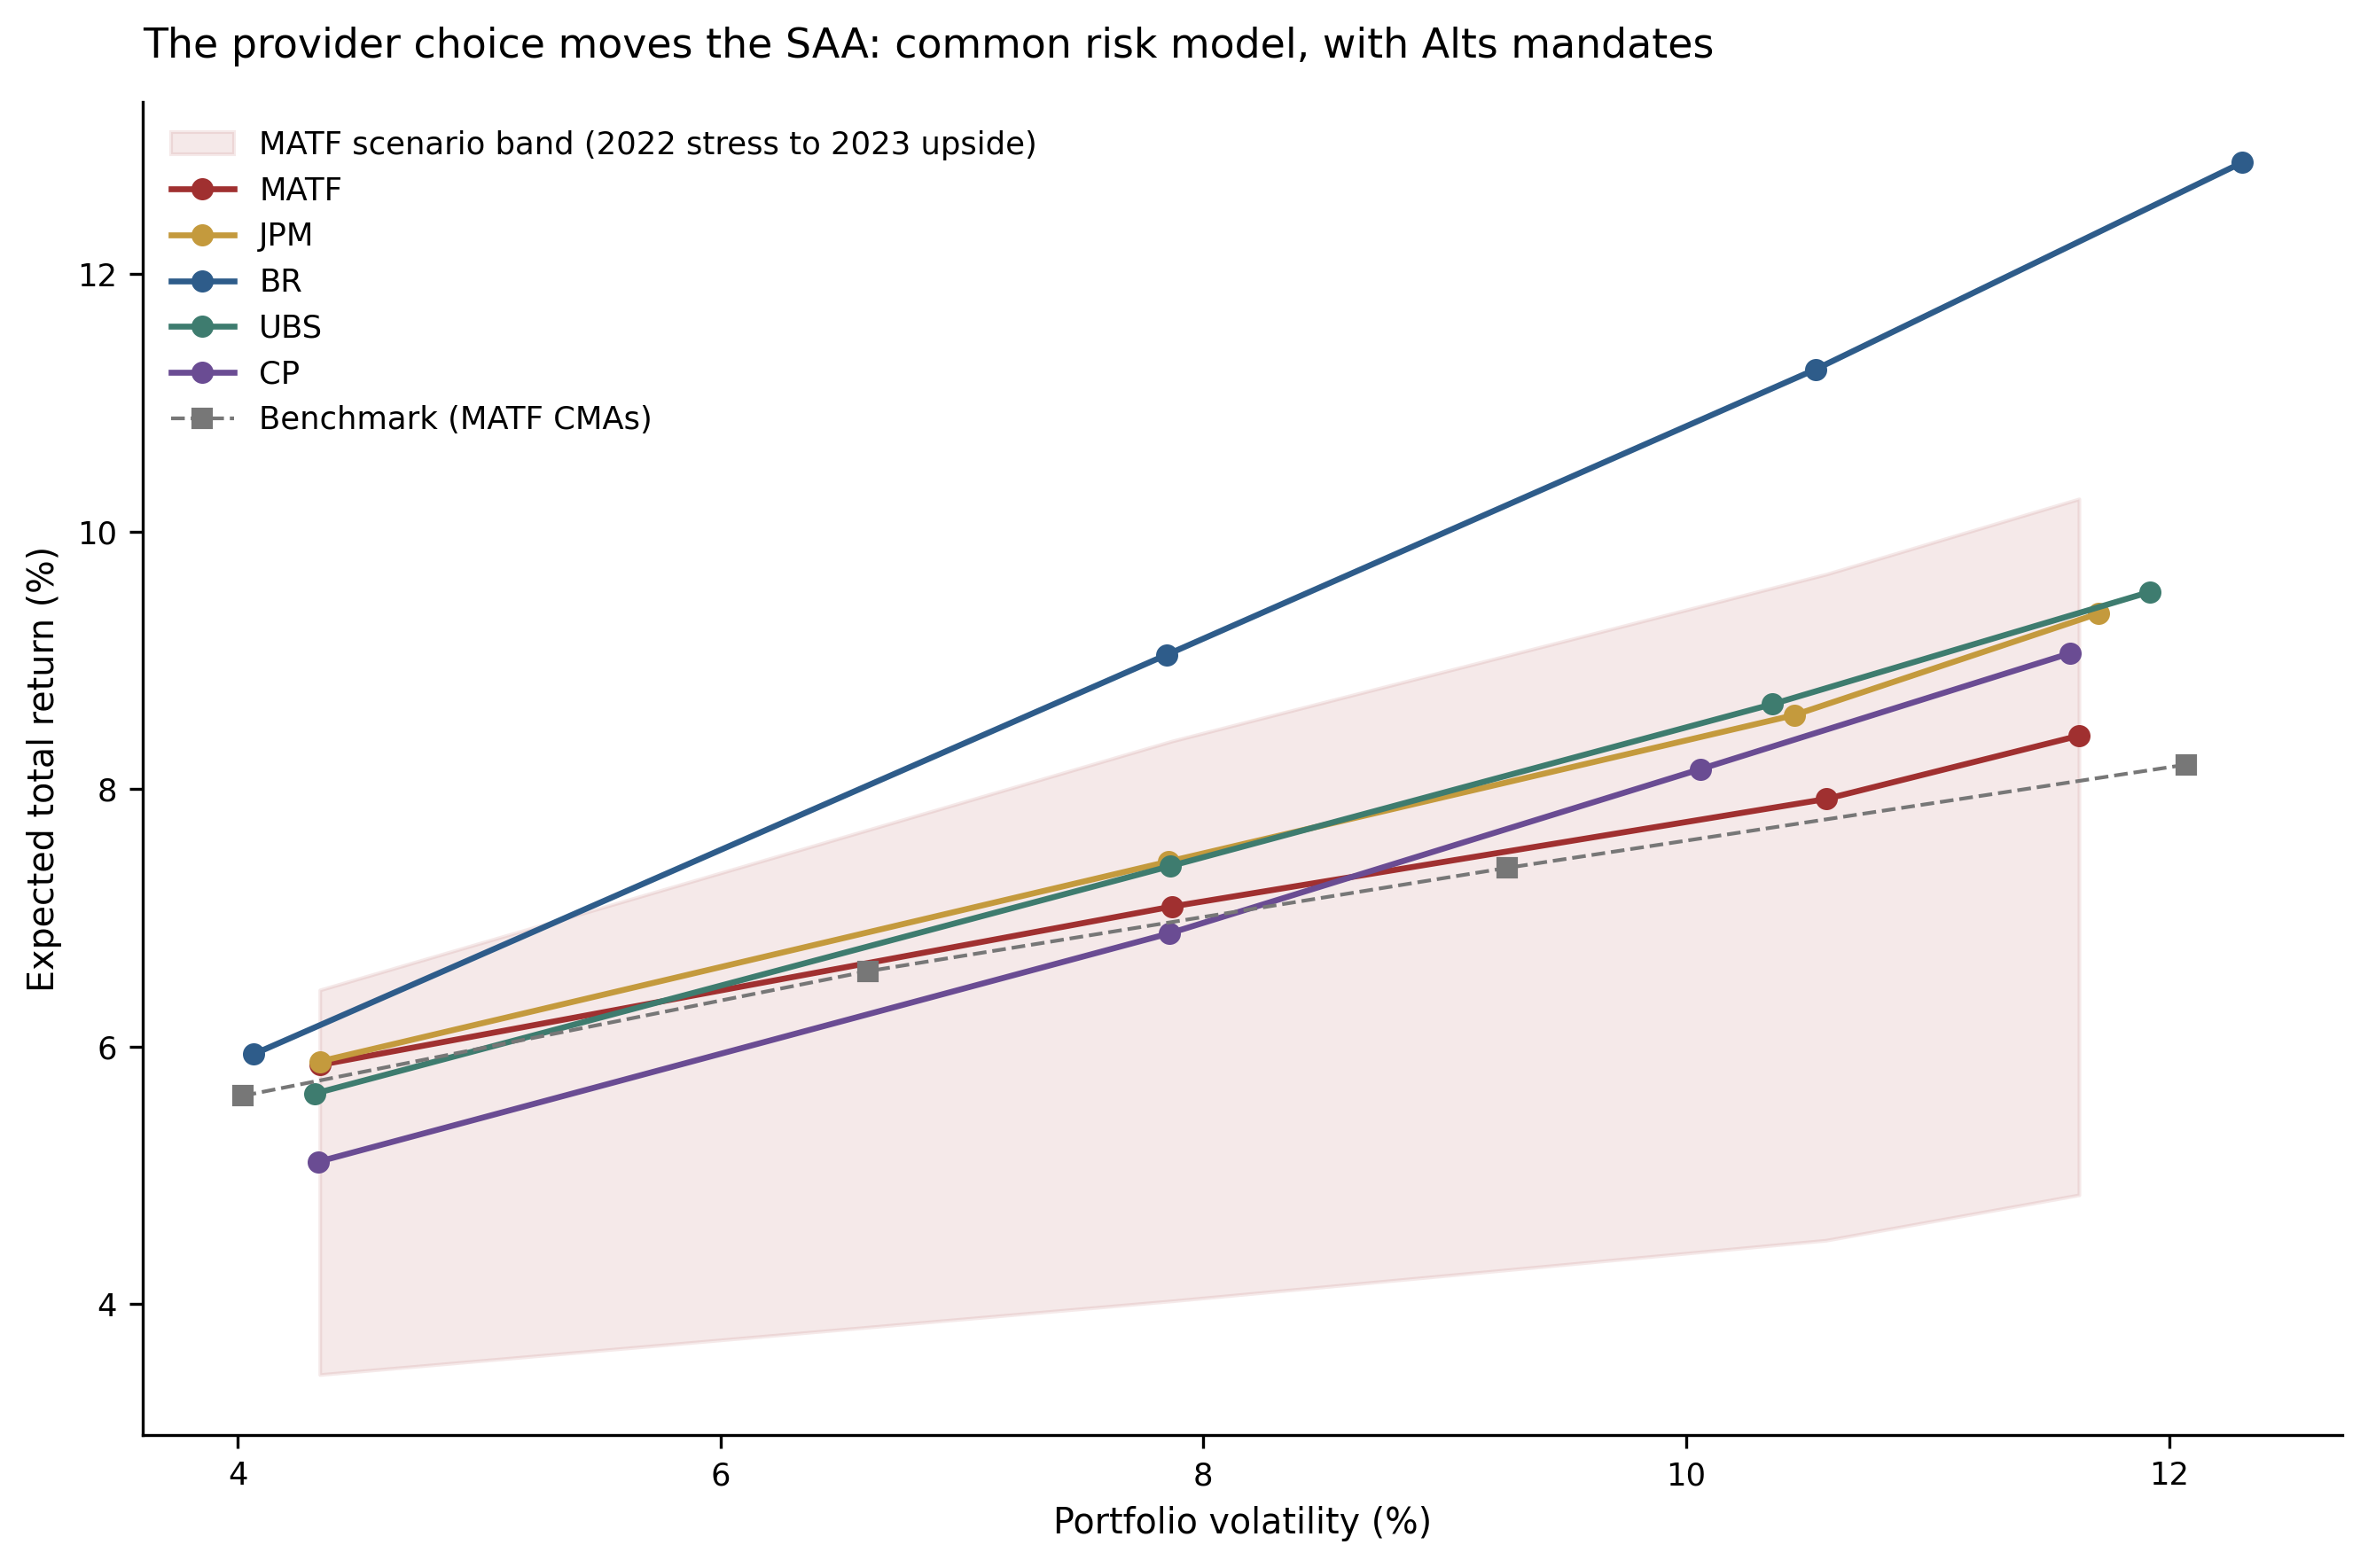
\includegraphics[width=0.8\linewidth]{figures/provider_frontier_with_alts.PNG}
		\end{center}
		\vspace*{-1.0\baselineskip}
		{\footnotesize Notes: with-Alternatives mandate family (Income, Low, Balanced, Growth), 2026-Q2 cut, USD, arithmetic total returns. Each provider's points are the TE-constrained optima of Exhibit~\ref{tab:provider_saa}'s design per mandate. The shaded band reprices the base-optimized MATF portfolios under the 2022-stress and 2023-upside factor shocks. The w/o-Alternatives family appears in Appendix~F.}
	\end{figure}
	
	The implication for the committee is attribution, not superiority. A provider choice under per-asset CMAs is a choice between black boxes. Under the MATF construction the committee can place any provider's numbers against the waterfall of Exhibit~\ref{fig:construction_waterfall} and the consistency diagnostic of Appendix~A, and it can express a preference for a provider's view as an explicit premium or admission adjustment rather than as a wholesale switch. The 0.65 to 0.74\% gap to the mainstream providers is also the quantity that consultants press upon, and the next section prices the only channel through which the framework lets that pressure act.
	
	% ===== END section3_provider.tex =====
	
	% ===== BEGIN section4_alpha_admission.tex =====
	% ======================================================================
	% SECTION 4 — DECISION TWO: THE ALPHA ADMISSION
	% Drop-in for the R2 inverted structure. Template: cma_paper_v4.tex.
	% Data freeze: 2026-Q2 production cut, 18 assets, PE MSCI at w = 0.5.
	% Figures map from the exhibit build:
	%   figures/admission_dial.PNG        <- exhibit_c8_admission_dial.png
	%   figures/admission_dial_nobox.PNG  <- exhibit_c8b_admission_dial_nobox.png
	% Bib entries required:
	%   SeppKastenholzFAJ2026  Sepp, A., and M. A. Kastenholz. "Achievable
	%     Sharpe and Universe Selection: A Closed-Form Factor Decomposition."
	%     Under review at the Financial Analysts Journal.
	%   MalkielSaha2005  [TODO: confirm entry] Malkiel, B. G., and A. Saha.
	%     2005. "Hedge Funds: Risk and Return." Financial Analysts Journal 61(6).
	% ======================================================================
	
	\sectionfont{\MakeUppercase}
	\section*{Decision Two: The Alpha Admission}\label{sec:admission}
	
	Alternatives carry the largest CMA disagreements and the strongest external pressure. The provider comparison of the previous section quantifies the pressure: on the Balanced mandate, matching the J.P. Morgan or UBS assumptions requires 65 to 74 basis points of additional expected return. Consultants translate such gaps into requests for higher alternatives assumptions. The MATF-CMA framework accepts such requests through exactly one channel. The Investment Committee sets the admission weight $w_i \in [0,1]$ of Equation~\eqref{eq:cma2a}, and the published workbook logs the admitted alpha $w_i \alpha_i$ for every asset.\footnote{A separate gross add-on channel converts selected fund CMAs to a gross-of-fee basis where consultants require gross numbers. The add-on is a reporting convention rather than a return view, so all analysis in this section holds it fixed. The add-on is zero on the paper universe.} Under per-asset construction the same request disappears into adjustments that no diagnostic can attribute. This section prices the dial. We show what the admission does to the allocation, what it does to the reported numbers, and which controls keep it defensible.
	
	\subsection*{The Admission Dial}\label{subsec:admission_dial}
	
	We scale the admitted alpha of every sleeve by a common factor $s$ and re-solve the Balanced mandate at each value. The CMA vector $\boldsymbol\mu(s)$ replaces each admitted alpha $w_i \alpha_i$ with $s \cdot w_i \alpha_i$ and holds every other CMA component fixed. The value $s=0$ is the pure factor book, $s=1$ is the production policy, and $s>1$ is the direction of consultant pressure. The optimization uses the constraints of the SAA application: weights within $\pm 50\%$ of the benchmark and tracking error capped at $1.5\%$.
	
	Exhibit~\ref{fig:admission_dial} reports the sweep. At $s=0$ the mandate claims an ex-ante excess Sharpe ratio of $0.30$. The production admission lifts the claim to $0.35$, and scaling one half beyond production lifts it to $0.39$. The optimal weights barely move, because the box and the tracking-error cap hold total alternatives near $37\%$ at every scale. Private Equity sits at its $22.5\%$ box cap throughout, so its admission changes no allocation and only raises the reported number. The composition rotates underneath: Private Credit moves from cap to floor, while Insurance-Linked and Gold move from floor to cap. The one-at-a-time sensitivity in Appendix~E ranks the individual assumptions. The Gold and Private Equity admissions move the claimed Sharpe ratio most, by $0.05$ and $0.06$ respectively, and the Private Equity admission at $w=0$ is the only setting that releases a sleeve from its box cap. The conclusion is uncomfortable and precise. The mandate guardrails contain the portfolio. Nothing in the optimization contains the claim.
	
	\begin{figure}[H]
		\captionof{figure}{The Admission Dial: Claimed Sharpe Rises While Guardrails Hold the Allocation}\label{fig:admission_dial}\vspace*{-0.5\baselineskip}
		\begin{center}
			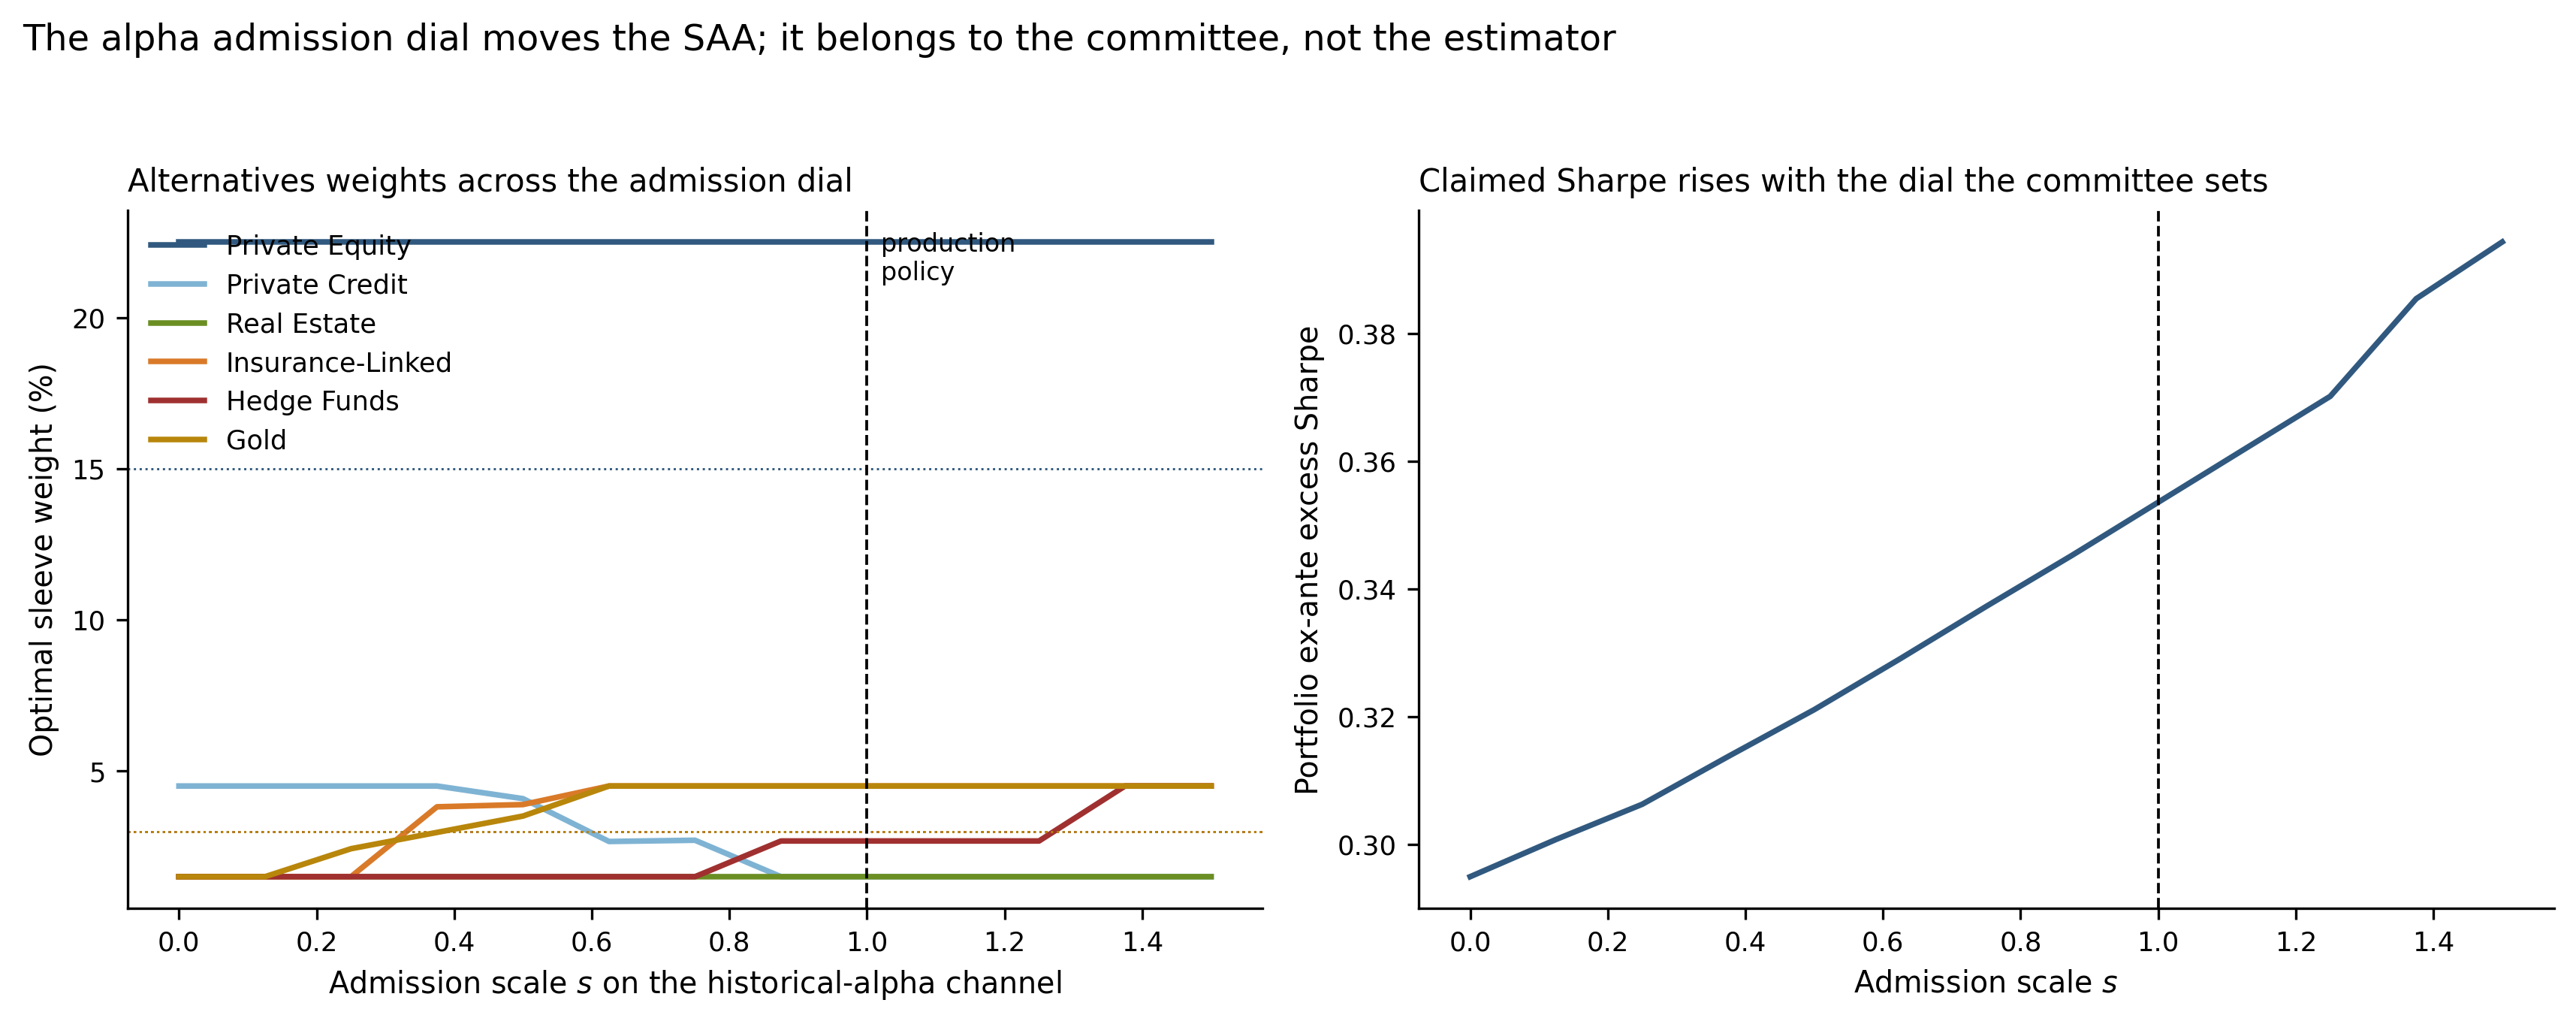
\includegraphics[width=0.95\linewidth]{figures/admission_dial.PNG}
		\end{center}
		\vspace*{-1.0\baselineskip}
		{\footnotesize Notes: Balanced with Alternatives mandate, 2026-Q2 production cut, USD. Left panel: optimal alternatives sleeve weights across the admission scale $s$ applied to the historical-alpha channel, with benchmark weights dotted. Right panel: claimed ex-ante excess Sharpe ratio of the optimal portfolio. Constraints: $\pm 50\%$ box around benchmark weights, $1.5\%$ tracking-error cap. The dashed line marks the production policy ($s=1$).}
	\end{figure}
	
	\subsection*{What the Guardrails Prevent}\label{subsec:admission_nobox}
	
	The dial shows its full force when the guardrails come off. We re-solve the allocation long-only at the benchmark volatility of $9.3\%$, with no box and no tracking-error constraint, on the identical risk model. Exhibit~\ref{fig:admission_nobox} reports the result. At the production admission the optimizer places $78\%$ of the book in alternatives, with $51\%$ in Private Equity and $22\%$ in Insurance-Linked. At $s=1.5$ it drops Private Equity entirely and corners into Insurance-Linked at $53\%$ and Gold at $47\%$. The corner migrates to whichever admission is scaled hardest. The claimed Sharpe ratio reaches $0.51$ at production and $0.77$ at $s=1.5$, against $0.35$ and $0.39$ under the mandate constraints.
	
	Two lessons follow. First, box and tracking-error constraints are not bureaucratic frictions but the binding defense against admitted-alpha concentration. Second, the admission must be governed per sleeve, because a cap on total alternatives would merely select which corner the optimizer takes.
	
	\begin{figure}[H]
		\captionof{figure}{Without Box and Tracking-Error Constraints, the Admission Corners the Book}\label{fig:admission_nobox}\vspace*{-0.5\baselineskip}
		\begin{center}
			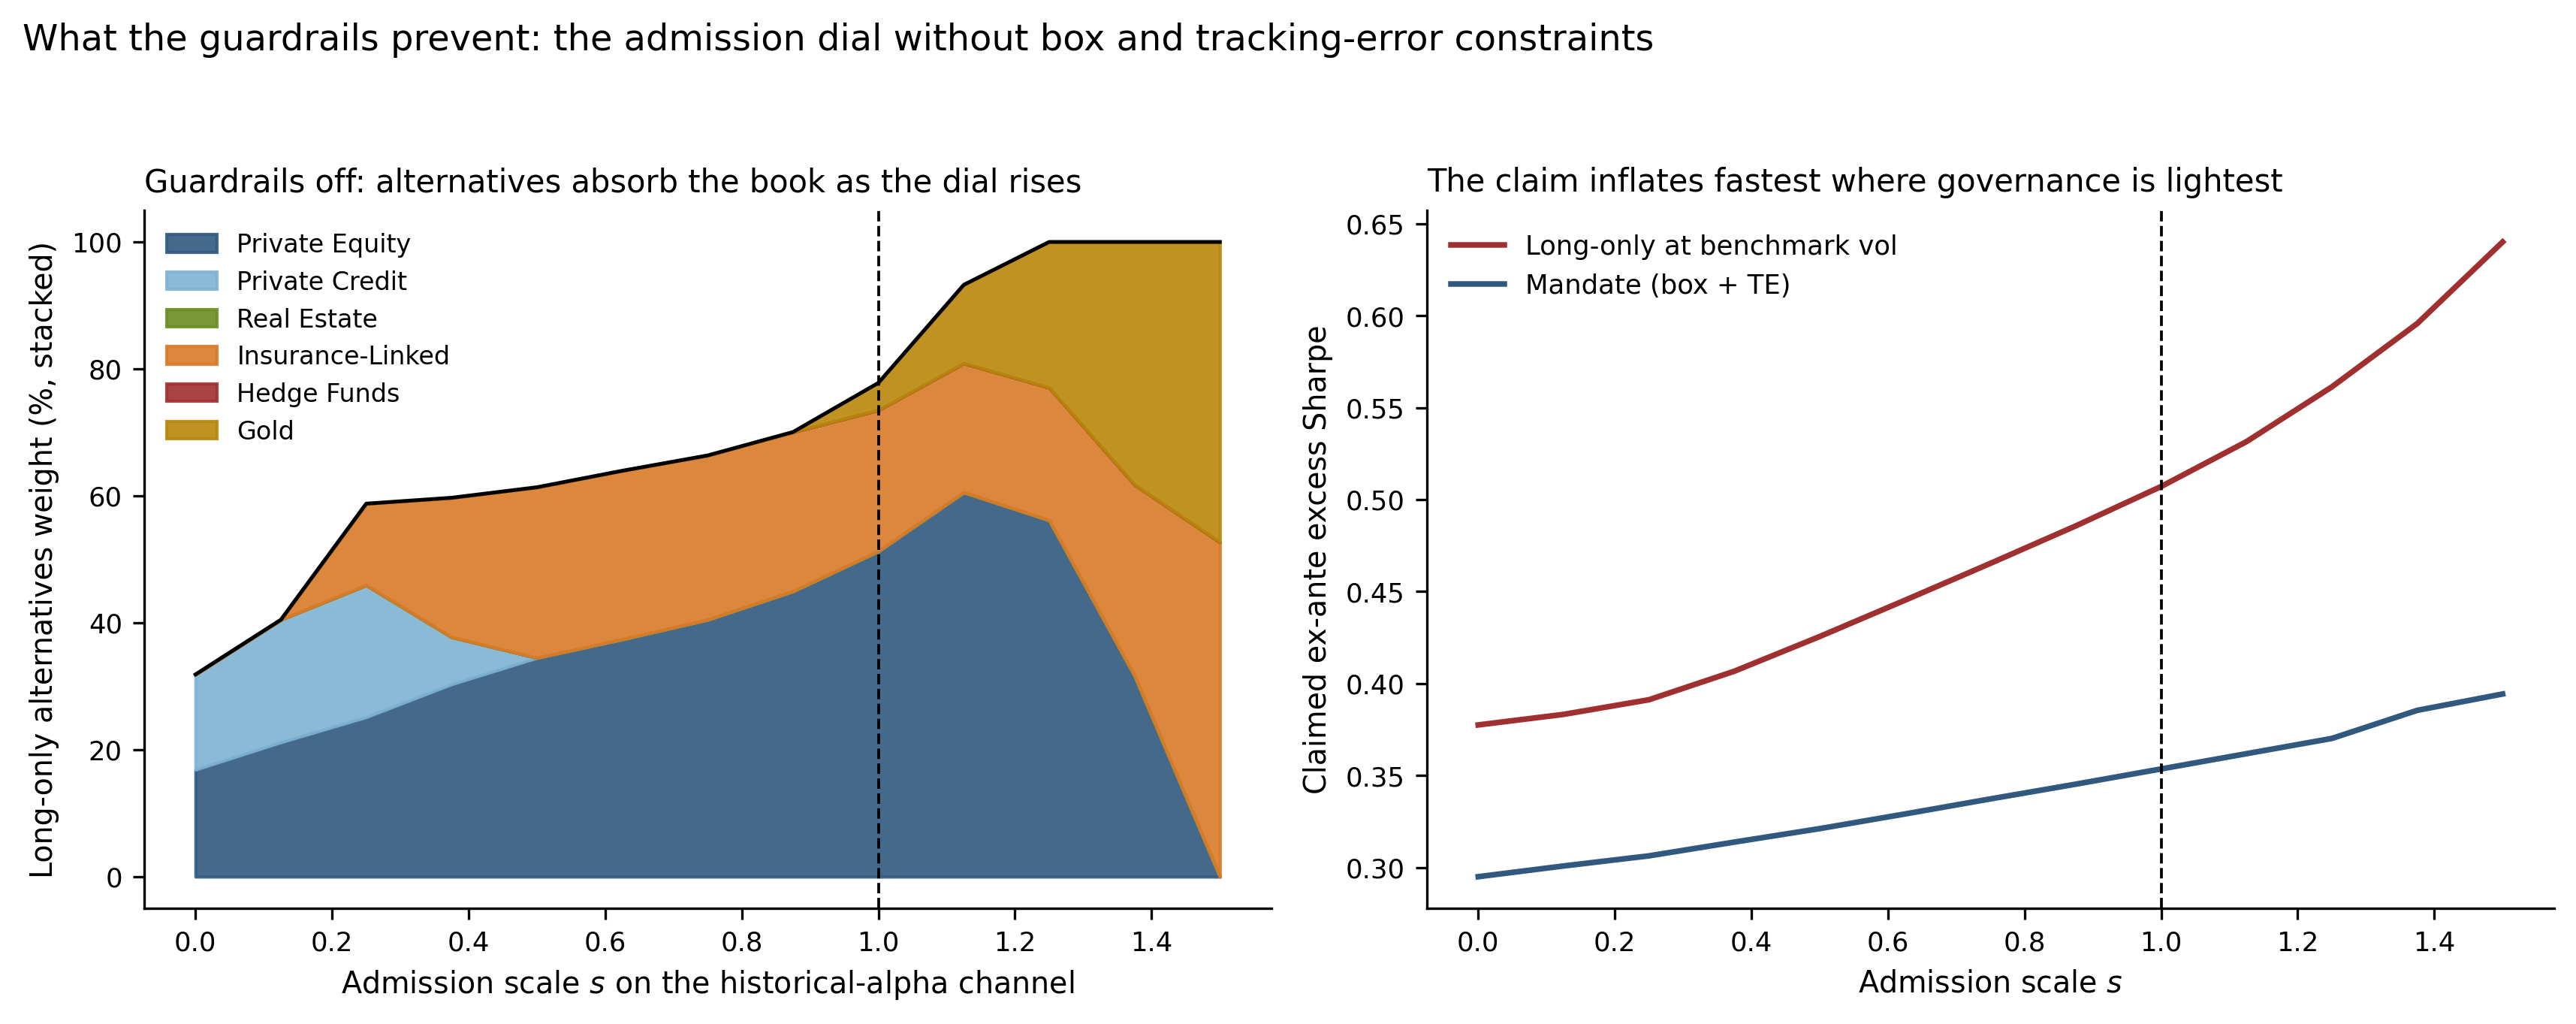
\includegraphics[width=0.95\linewidth]{figures/admission_dial_nobox.PNG}
		\end{center}
		\vspace*{-1.0\baselineskip}
		{\footnotesize Notes: long-only maximum-return allocation at the benchmark volatility target of $9.3\%$, 2026-Q2 production cut, USD, same risk model as Exhibit~\ref{fig:admission_dial}. Left panel: stacked alternatives weights across the admission scale $s$. Right panel: claimed ex-ante excess Sharpe ratio with the guardrails off (red) against the mandate solution of Exhibit~\ref{fig:admission_dial} (blue).}
	\end{figure}
	
	\subsection*{What the Admission Buys}\label{subsec:admission_sr2}
	
	Admission weights claim idiosyncratic Sharpe content, and the claim can be priced. \citet{SeppKastenholzFAJ2026} decompose the squared Sharpe ratio of the optimal portfolio into a systematic component, attainable from factor premia through the given asset universe, and an idiosyncratic component carried by admitted alpha. On the frozen production cut, the nine factor premia offer a frictionless squared Sharpe ratio of $0.57$, of which the 18-asset universe makes $0.24$ attainable. The raw production admissions claim an idiosyncratic squared Sharpe ratio of $1.40$, which is more than twice the entire factor opportunity set. A generalized-least-squares projection strips the component of admitted alpha that is factor premium in disguise, and the honest claim drops to $0.63$. The projection also attributes the disguise per sleeve: $84\%$ of the Private Equity admission and $77\%$ of the Private Credit admission are premium-like, against $30\%$ for Hedge Funds and $29\%$ for Gold. We read the Private Equity share as independent confirmation of appraisal smoothing, because the cross-sectional projection reaches the same verdict as cash-flow-based loading estimates by a different route.
	
	Even the honest $0.63$ exceeds everything the factor set can deliver through these assets. A committee that signs the production admissions therefore asserts more skill content than systematic content in the book. The assertion may be right. It should at least be visible, and the next subsection makes it testable.
	
	\subsection*{Two Auditable Caps}\label{subsec:admission_caps}
	
	Visibility invites control. We propose two caps that turn the admission policy into pass-fail tests a validator can run from the published workbook. Cap~1 bounds the admitted information ratio, $w_i \alpha_i / \sigma_{\varepsilon,i} \le 0.50$, at the maximum factor Sharpe prior in the framework: no sleeve should claim more reward per unit of residual risk than the best-rewarded systematic factor. Cap~2 bounds the above-factor share of the excess CMA at $50\%$, so that factor economics remain the primary driver of every published assumption. We believe the two caps are the right minimal control set because each targets a distinct failure. Cap~1 targets the over-claiming of skill, and Cap~2 targets the crowding-out of factor economics. Exhibit~\ref{tab:admission_audit} reports the production policy against both.
	
	\begin{table}[H]
		\captionof{table}{Alpha Admission Policy Audit with Two Governance Caps}\label{tab:admission_audit}\vspace*{-0.5\baselineskip}
		\begin{center}
			\footnotesize
			\begin{tabular}{l rrrr rr cc}
				\toprule
				Sleeve & $w_i$ & $\alpha_i$ & $w_i\alpha_i$ & Excess CMA & Share & IR & Cap 1 & Cap 2 \\
				& & (\%) & (\%) & (\%) & (\%) & & IR $\le 0.50$ & Share $\le 50\%$ \\
				\midrule
				Private Equity   & 0.50 & 2.80  & 1.40 & 4.94 & 28 & 0.19 & pass & pass \\
				Private Credit   & 0.50 & 1.85  & 0.93 & 3.08 & 30 & 0.19 & pass & pass \\
				Real Estate      & 0.00 & $-2.48$ & 0.00 & 2.21 & 0  & 0.00 & pass & pass \\
				Insurance-Linked & 1.00 & 3.58  & 3.58 & 3.85 & 93 & 0.83 & FAIL & FAIL \\
				Hedge Funds      & 1.00 & 2.04  & 2.04 & 3.25 & 63 & 0.77 & FAIL & FAIL \\
				Gold             & 0.25 & 13.93 & 3.48 & 4.50 & 77 & 0.23 & pass & FAIL \\
				\bottomrule
			\end{tabular}
		\end{center}
		\vspace*{-0.5\baselineskip}
		{\footnotesize Notes: 2026-Q2 production cut, USD, excess returns in percent per annum. $\alpha_i$ is the statistical Jensen alpha of Equation~\eqref{eq:jensen}, $w_i$ the admission weight, and Share the ratio of declared above-factor adjustments to the excess CMA. IR is the admitted information ratio $w_i \alpha_i / \sigma_{\varepsilon,i}$ with $\sigma_{\varepsilon,i}$ the residual volatility of the risk model. The gross add-on channel is zero on this universe and omitted.}
	\end{table}
	
	The caps have already changed the policy once. The Private Equity sleeve entered the quarter at full admission and passed Cap~1 with an information ratio of $0.37$. The pass was uninformative, because Cap~1 tests magnitude while the $84\%$ premium-like share above is an identification failure. We therefore recut the admission to $w=0.5$, and the sleeve now passes both caps with an information ratio of $0.19$ and an above-factor share of $28\%$. The episode fixes the caps' place in the control set: they are necessary and not sufficient. Sleeves with appraisal-suspect return histories therefore carry a weight discount on top of the cap tests.
	
	Two production sleeves still fail. Insurance-Linked at full admission carries an information ratio of $0.83$ and an above-factor share of $93\%$. Hedge Funds at full admission carry $0.77$ and $63\%$, on an index with documented survivorship and backfill bias \citep{MalkielSaha2005}. Gold passes the information-ratio cap at $0.23$ and fails the share cap at $77\%$. We report the failures rather than resolve them silently, because a printed failure is the audit working as designed and the input to the next policy debate. Insurance-Linked is the limit case worth stating plainly. With $R^{2}=0.17$ against the factor set, the sleeve is held almost entirely on non-factor grounds, and the framework says so in one row of Exhibit~\ref{tab:admission_audit}. A building-block CMA would make the same bet silently, inside an unattributable per-asset assumption.
	
	The multi-advisor consensus corroborates the caps from an independent direction. The survey of \citet{HorizonSurvey2025} makes no adjustment for active-manager alpha, so its 41-advisor averages benchmark the pure market-return book, which is the $s=0$ comparator of Exhibit~\ref{fig:admission_dial}. Without admitted alpha, every MATF alternatives sleeve sits at or below the survey median. The production admissions lift exactly two sleeves above the survey's 75th percentile, Hedge Funds at $7.2\%$ geometric against a survey distribution ending at $8.5\%$, and Gold at $7.1\%$ against a commodities distribution ending at $7.5\%$.\footnote{The survey's commodities line covers broad commodity baskets rather than gold specifically, so the Gold placement is indicative. The recut Private Equity assumption sits just below the survey's 25th percentile, so the identification discipline of the recut positions the sleeve conservatively against the 41-advisor consensus.} The two sleeves the external consensus flags are the two sleeves the internal caps flag, by entirely different routes.
	
	The implication for practice is a change in what the committee debates. Under per-asset construction the alternatives discussion is a negotiation over dozens of correlated return numbers. Under MATF-CMA it is a decision over one weight per sleeve, priced in claimed Sharpe by Exhibit~\ref{fig:admission_dial}, bounded by the caps of Exhibit~\ref{tab:admission_audit}, and reconciled line by line to the published workbook. External pressure to raise alternatives expectations does not disappear. It arrives at a governed dial with the trade-off stated, which is where an Investment Committee can exercise judgment.
	
	% ===== END section4_alpha_admission.tex =====
	
	% ===== BEGIN section5_scenarios.tex =====
	% ======================================================================
	% SECTION 5 — DECISION THREE: COHERENT SCENARIOS
	% Drop-in for the R2 inverted structure. Template: cma_paper_v4.tex.
	% Source: v4 subsection "Scenario-Based CMA Adjustments" (lines 823-868),
	% promoted to a section, tightened, and extended with the scenario-admission
	% interaction (Exhibit C12) per the signed-off outline.
	% Data freeze: 2026-Q2 production cut, 18 assets, PE MSCI at w = 0.5.
	% Figures map from the exhibit build:
	%   figures/scenario_admission.PNG <- exhibit_c12_scenario_admission.png
	% External labels referenced (defined in other sections of the manuscript):
	%   fig:provider_frontier  (Section 3, Exhibit B5 with the scenario band)
	%   fig:admission_dial     (Section 4)
	%   tab:admission_audit    (Section 4)
	% ======================================================================
	
	\sectionfont{\MakeUppercase}
	\section*{Decision Three: Coherent Scenarios}\label{sec:scenarios}
	
	Strategic asset allocation requires stress and upside cases in addition to the base CMAs, and the committee must decide in which language to approve them. Defining scenarios asset by asset is ad hoc and risks internal inconsistency: a stress table with equities down, credit unchanged, and hedge funds flat encodes cross-asset claims that nobody has checked. We instead define every scenario as one vector of factor shocks and let the loading matrix reprice all assets. The construction guarantees that factor co-movements are empirically consistent, because the shocks are realized returns from historical episodes.
	
	Historical factor returns are annual realizations, while the CMAs operate on a 5--10 year horizon. We de-compound the annual factor return over the CMA horizon:
	\begin{equation}\label{eq:decompound}
		\Delta f_k^{5Y} = \frac{1}{T} \cdot f_k^{annual,scenario},
	\end{equation}
	where $T=5$ is the CMA horizon. The scenario CMA for asset $i$ is then
	\begin{equation}\label{eq:cma_scenario}
		\text{CMA}_i^{scenario} = \underbrace{\text{CMA}_i^{base}}_{\text{Equation~\eqref{eq:cma2}}} + \underbrace{\hat{\boldsymbol\beta}_i^{\intercal} \Delta \boldsymbol f^{5Y}}_{\text{scenario adjustment}}.
	\end{equation}
	The adjustment is additive on the base CMA, so declared adjustments carry into every scenario unchanged. The replication code asserts the additive identity on the published workbook at each production cut.
	
	We select 2022 as the stress scenario, with a simultaneous equity and rates sell-off, and 2023 as the upside scenario, with an equity and credit recovery. Exhibit~\ref{tab:factor_returns} reports the annual factor returns and the de-compounded bumps. The committee approves nine numbers per scenario, and every asset-level and mandate-level consequence follows mechanically. Additional scenarios from other reference episodes, such as 2008, 2019, or 2020, are constructed the same way.
	
	\begin{table}[H]
		\captionof{table}{One Factor-Shock Vector Defines Each Scenario: MATF Excess Returns for the Scenario Years and De-Compounded 5Y Bumps}\label{tab:factor_returns}\vspace*{-1.0\baselineskip}
		\begin{center}
			\small
			\begin{tabular}{lrrrrrr}
				\toprule
				& \multicolumn{2}{c}{\textbf{Annual return (\%)}} & & \multicolumn{2}{c}{\textbf{5Y bump (\%)}} \\
				\cmidrule{2-3} \cmidrule{5-6}
				\textbf{Factor} & \textbf{2022} & \textbf{2023} & & \textbf{Stress} & \textbf{Upside} \\
				& & & & (2022) & (2023) \\
				\midrule
				Equity        & $-19$ & $+15$ & & $-3.8$ & $+3.0$ \\
				Rates         & $-16$ & $+0$  & & $-3.2$ & $+0.0$ \\
				Credit        & $-1$  & $+7$  & & $-0.2$ & $+1.4$ \\
				Carry         & $+1$  & $+2$  & & $+0.2$ & $+0.4$ \\
				Inflation     & $+4$  & $-1$  & & $+0.8$ & $-0.2$ \\
				Commodities   & $+13$ & $-10$ & & $+2.6$ & $-2.0$ \\
				PE            & $-4$  & $+5$  & & $-0.8$ & $+1.0$ \\
				Rates Vol     & $+5$  & $-1$  & & $+1.0$ & $-0.2$ \\
				FX            & $+12$ & $-1$  & & $+2.4$ & $-0.2$ \\
				\bottomrule
			\end{tabular}
		\end{center}
		\vspace*{-0.5\baselineskip}
		{\footnotesize Notes: annual excess returns of the MATF factors realized in 2022 and 2023, and the corresponding 5-year scenario bumps of Equation~\eqref{eq:decompound}. Source: production factor histories, 2026-Q2 cut.}
	\end{table}
	
	Scenario repricing is evaluation-only. We hold the base-optimized portfolios fixed and reprice them under each shock vector, because a stress test measures the book the committee holds rather than a book it would hold with foresight of the stress. On the Balanced mandate with alternatives, the base total CMA of $7.9\%$ reprices to $9.7\%$ under the 2023 upside and $4.5\%$ under the 2022 stress. The scenario band across all eight mandates appears in Exhibit~\ref{fig:provider_frontier}, where it also frames the cross-provider dispersion: the CMA disagreement between mainstream providers is small relative to the scenario range the committee should hold in mind.
	
	The scenario machinery interacts with the alpha admission of the previous section in one specific way. Factor premia shock under a scenario, and admitted alpha does not, because the admission sits inside the base CMA of Equation~\eqref{eq:cma_scenario}. Exhibit~\ref{fig:scenario_admission} traces the consequence across the admission dial. The width of the scenario band stays near $5.2\%$ at every admission scale, while the whole band shifts up with the admitted-alpha carry. At zero admission the Balanced stress case reads an excess return of $-0.3\%$, and at the production admission it reads $+0.3\%$. The sign of the reported stress outcome flips purely on the assumption that the admitted skill survives a repeat of 2022, and the admitted-alpha carry accounts for essentially all of the improvement. We do not judge the assumption here. We insist only that the committee sees it: the stress report belongs at the factor level, where the admission carry is separated from the factor repricing, rather than at the headline level where the two are mixed.
	
	\begin{figure}[H]
		\captionof{figure}{Admitted Alpha Does Not Shock: Rising Admission Flatters the Stress Case One-for-One}\label{fig:scenario_admission}\vspace*{-0.5\baselineskip}
		\begin{center}
			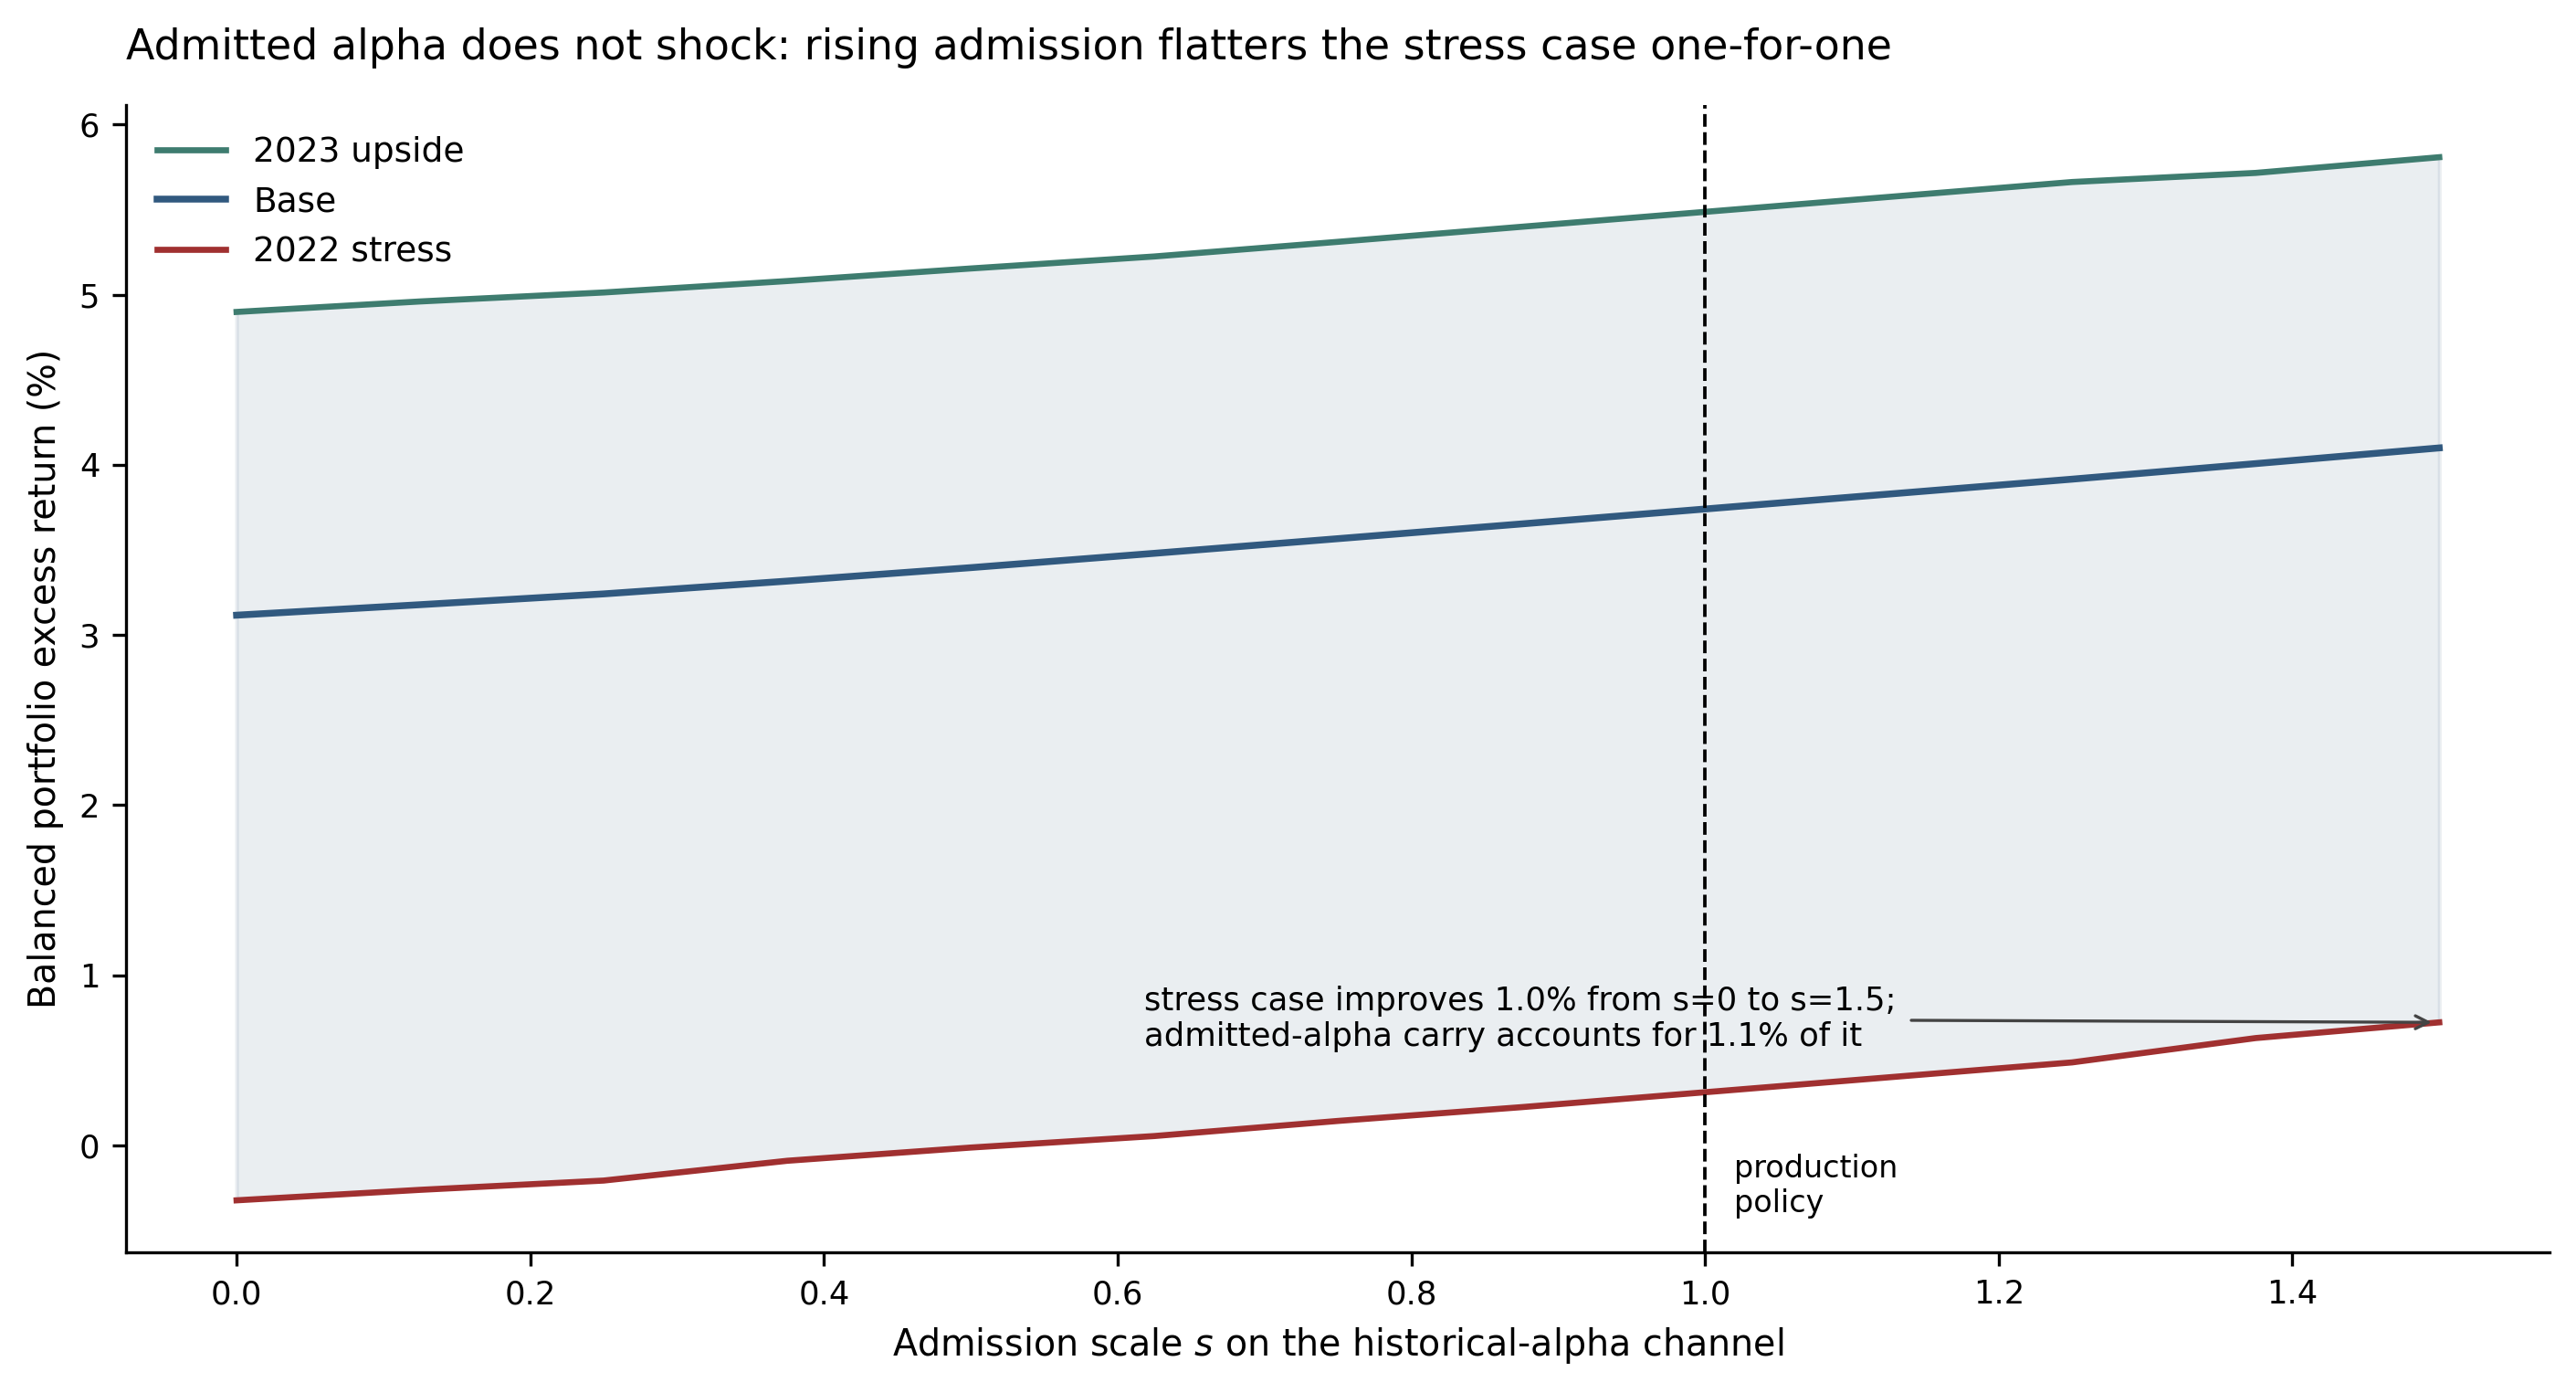
\includegraphics[width=0.75\linewidth]{figures/scenario_admission.PNG}
		\end{center}
		\vspace*{-1.0\baselineskip}
		{\footnotesize Notes: Balanced with Alternatives mandate, 2026-Q2 production cut, USD, excess returns in percent per annum. Each point re-solves the mandate at admission scale $s$ under the constraints of Exhibit~\ref{fig:admission_dial} and reprices the optimal book under the 2022 stress and 2023 upside shock vectors of Exhibit~\ref{tab:factor_returns}. The dashed line marks the production policy.}
	\end{figure}
	
	The implication for governance mirrors the previous section. The scenario debate reduces to nine factor shocks per episode, approved once and applied everywhere, and the stress report separates what markets do to the book from what the committee has assumed about skill. Under per-asset construction both statements are unavailable, because the scenario table and the alpha assumptions are fused inside the same hand-set numbers.
	
	% ===== END section5_scenarios.tex =====
	
	% ===== BEGIN section6_trust.tex =====
	% ======================================================================
	% SECTION 6 — HOW MUCH TO TRUST THE NUMBERS
	% Drop-in for the R2 inverted structure. Template: cma_paper_v4.tex.
	% Source: v4 "Bootstrap Evidence" section (lines 1114-1207), compressed.
	% Bootstrap numbers regenerated on the 2026-Q2 18-asset freeze
	% (run_bootstrap_q2.py, B=500, window Jul 2001 - Jun 2026, seed 42,
	% Q2 SR prior [0.35,0.35,0.25,0.25,0.15,0.15,0.50,0.25,0.00], sigma_SR=0.10;
	% headline JSON: figures/bootstrap_headline_q2.json).
	% Analytic SE triple recomputed on Q2 inputs in Appendix B (3.24/3.64/1.53).
	% Figures:
	%   figures/bootstrap_frontier.PNG   <- bootstrap_frontier_q2.png [frozen Q2]
	%   figures/declared_delta.PNG       <- exhibit_a2_declared_delta.png [frozen Q2]
	% The SE-comparison table (v4 tab:se_comparison) moves to Appendix B.
	% ======================================================================
	
	\sectionfont{\MakeUppercase}
	\section*{How Much to Trust the Numbers}\label{sec:trust}
	
	The decisions of the previous three sections consume the CMAs as given. The committee's remaining question is calibration: how much of the expected performance is signal, and how much is estimation noise inherited from the inputs? The stake is practical. Under per-asset sample-mean CMAs, the policy benchmark itself sits inside the $90\%$ confidence band of the optimized frontier, so a CIO cannot statistically distinguish the proposed SAA from the benchmark on expected return alone. This section reports two audits: the sampling uncertainty of the frontier and the reconciliation of the consistency residual. Appendix~A develops the diagnostic and Appendix~B the bootstrap design.
	
	\subsection*{Estimation Uncertainty: The Frontier Bandwidth}\label{subsec:trust_bootstrap}
	
	The three CMA constructions carry very different sampling noise on the same data. The per-asset sample mean over an effective $25$ years of monthly returns has a standard error of $3.2\%$ for US equity. A Grinold-Kroner building-block construction is no better at $3.6\%$, because each component is a forecast of a separate process and the variance does not shrink with the sample. The MATF construction estimates $M=9$ factor Sharpe ratios jointly across the whole universe under an economic prior, and the same US-equity standard error falls to $1.5\%$. The prior dispersion of $\sigma_{SR}=0.10$ is empirically grounded: \citet{Lemperiere2017} document that long-run Sharpe ratios of well-identified risk premia cluster in a narrow band around $0.30$. The advantage is structural: the framework estimates fewer parameters using more data. Appendix~B derives the three standard errors and reports the $\sigma_{SR}$ sensitivity grid.
	
	Exhibit~\ref{fig:bootstrap_frontier} shows the consequence for the object the committee actually approves. Across $B=500$ stationary block-bootstrap draws of a $300$-month window of multi-asset returns, the $90\%$ bandwidth of the long-only frontier runs from $3.0\%$ to $8.0\%$ across the volatility grid under the per-asset estimator, and from $1.3\%$ to $4.6\%$ under MATF. The reduction is approximately $2\times$ across the mandate volatility range. The information gain is equivalent to roughly $4\times$ the historical sample, since sample-mean variance scales inversely with the sample size. The equivalence explains why per-asset SAA fails at realistic samples: \citet{DeMiguelGarlappiUppal2009} estimate that sample-mean mean-variance needs around $3{,}000$ months to beat equal weighting on $25$ assets, roughly ten times the record that exists. Forward-looking per-asset views shift the point estimate and not the uncertainty around it, so the bandwidth comparison extends to Grinold-Kroner constructions.
	
	\begin{figure}[H]
		\captionof{figure}{Factor Structure with an Economic Prior Halves the Frontier's Sampling Bandwidth}\label{fig:bootstrap_frontier}\vspace*{-0.5\baselineskip}
		\begin{center}
			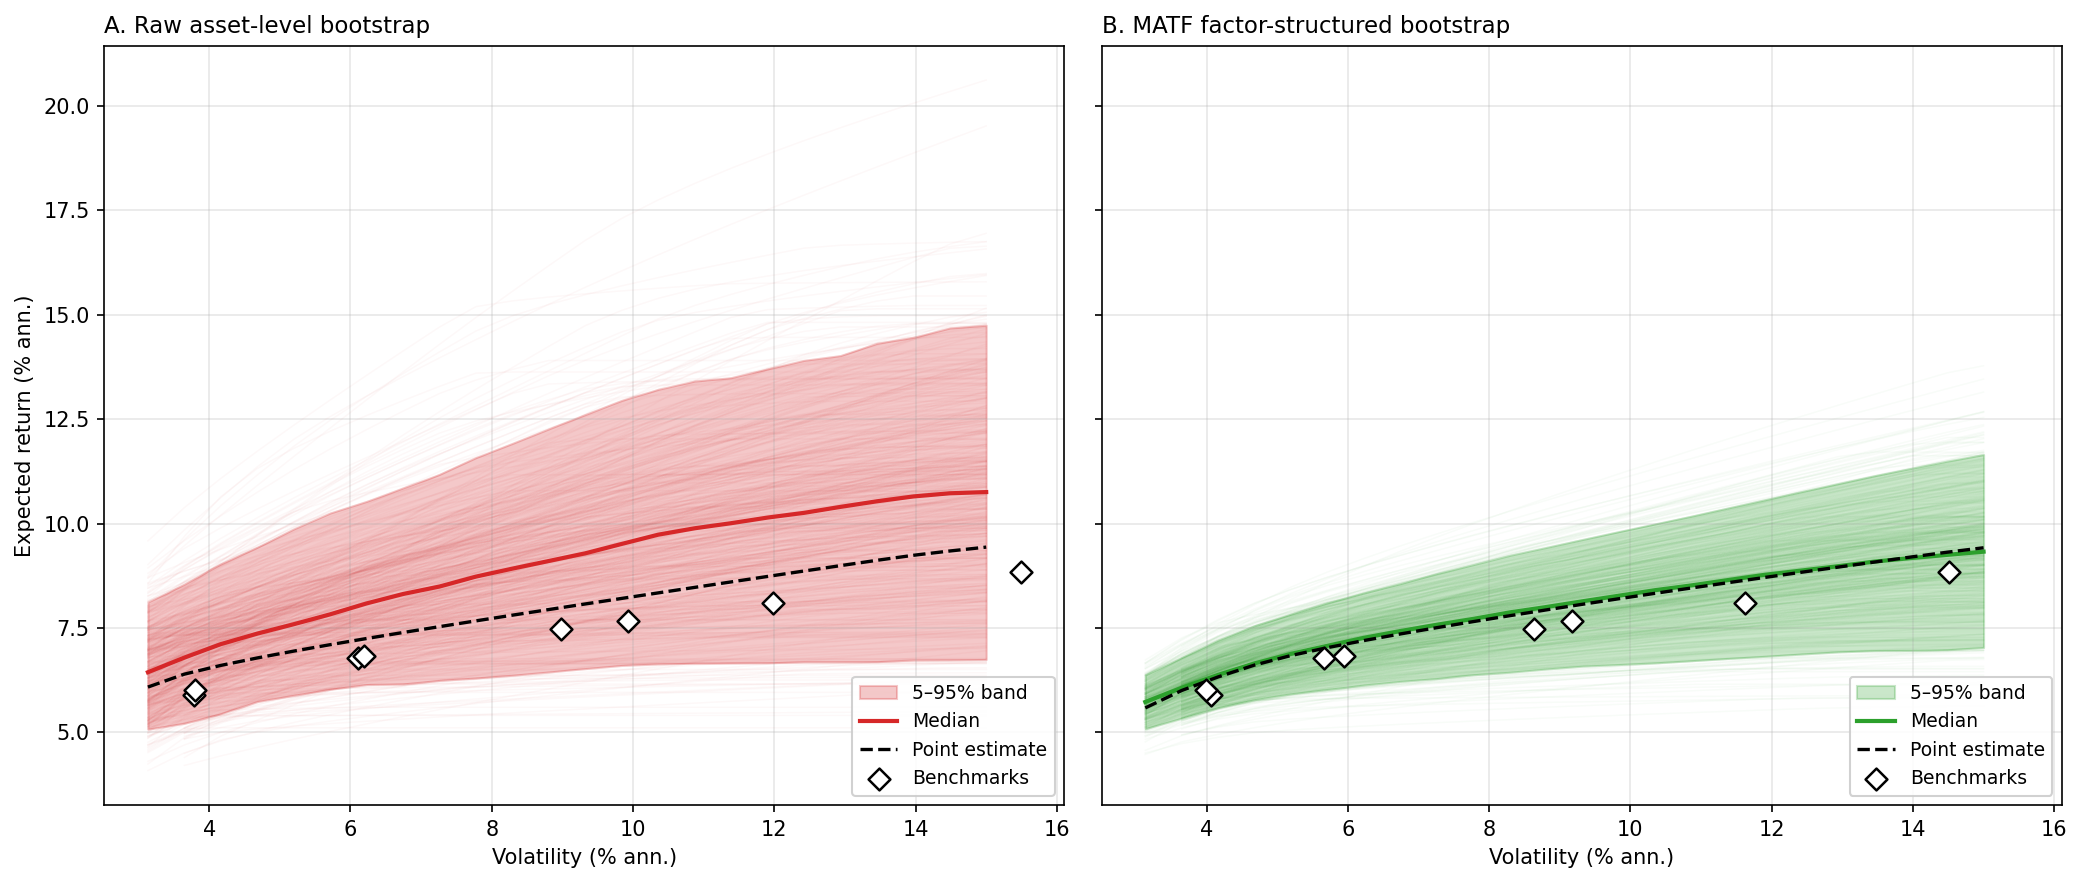
\includegraphics[width=0.97\linewidth]{figures/bootstrap_frontier.PNG}
		\end{center}
		\vspace*{-1.0\baselineskip}
		{\footnotesize Notes: bootstrap distribution of the long-only efficient frontier under the per-asset sample-mean estimator (Panel A) and the MATF estimator (Panel B), $B=500$ stationary block draws with mean block $12$ months on a $300$-month window (July 2001 to June 2026), 2026-Q2 cut, 18 assets. Shaded bands are the 5th--95th percentiles, solid lines the bootstrap medians, dashed lines the full-sample point estimates, and diamonds the eight policy mandates. Design in Appendix~B.}
	\end{figure}
	
	\subsection*{Consistency: Declared versus Unattributed Deviation}\label{subsec:trust_consistency}
	
	The second audit concerns the consistency residual itself. Appendix~A defines, for any excess-CMA vector $\boldsymbol\mu$ and any factor risk model, the residual $\boldsymbol\Delta(\boldsymbol\mu, \hat{\boldsymbol\beta})$ as the component of $\boldsymbol\mu$ the factor span cannot explain. The diagnostic is model-independent: it applies to any provider's CMAs against any loading matrix, with no knowledge of how either was constructed, which makes it the natural companion to the provider comparison of Section ``Decision One''.
	
	Under the MATF construction of Equation~\eqref{eq:cma2a}, the residual is not zero, and the framework does not claim it is. The residual equals the annihilated image of the declared channels, $\boldsymbol\Delta = \boldsymbol M_{\hat\beta}(\boldsymbol b + \boldsymbol W\boldsymbol\alpha + \boldsymbol a)$ with $\boldsymbol M_{\hat\beta}$ the annihilator of Appendix~A, because the annihilator removes the factor-implied component by construction. The claim is therefore exact reconciliation: every basis point of $\boldsymbol\Delta$ traces to a logged entry in the construction waterfall of Exhibit~\ref{fig:construction_waterfall}, and the replication code asserts the reconciliation on the published workbook at each production cut. On the frozen cut the maximum reconciliation gap is of the order $10^{-17}$, which is numerical zero.
	
	Per-asset constructions offer no such reconciliation. Exhibit~\ref{fig:declared_delta} compares the two on the frozen universe with identical loadings and residual variances. The historical-mean construction leaves unattributed residuals of up to $5.5\%$ per asset with a median near $0.5\%$, concentrated in the low-$R^2$ alternatives and the single-country equity sleeves. The bootstrap version of the same comparison in Appendix~B puts the portfolio-level violation norm at a median of $3.4\%$ across draws, with per-asset medians between roughly $30$ and $115$ basis points. The practical reading is the one from Section ``The Committee's Problem'': $64$ basis points of median unattributed residual on the insurance-linked sleeve is $64$ basis points the optimizer prices as alpha, and the alpha has no replication strategy behind it. The framework does not promise zero deviation. It promises zero unattributed deviation, and the promise is checked by machine rather than by assertion.
	
	\begin{figure}[H]
		\captionof{figure}{The Framework Promises Zero Unattributed Deviation, Not Zero Deviation}\label{fig:declared_delta}\vspace*{-0.5\baselineskip}
		\begin{center}
			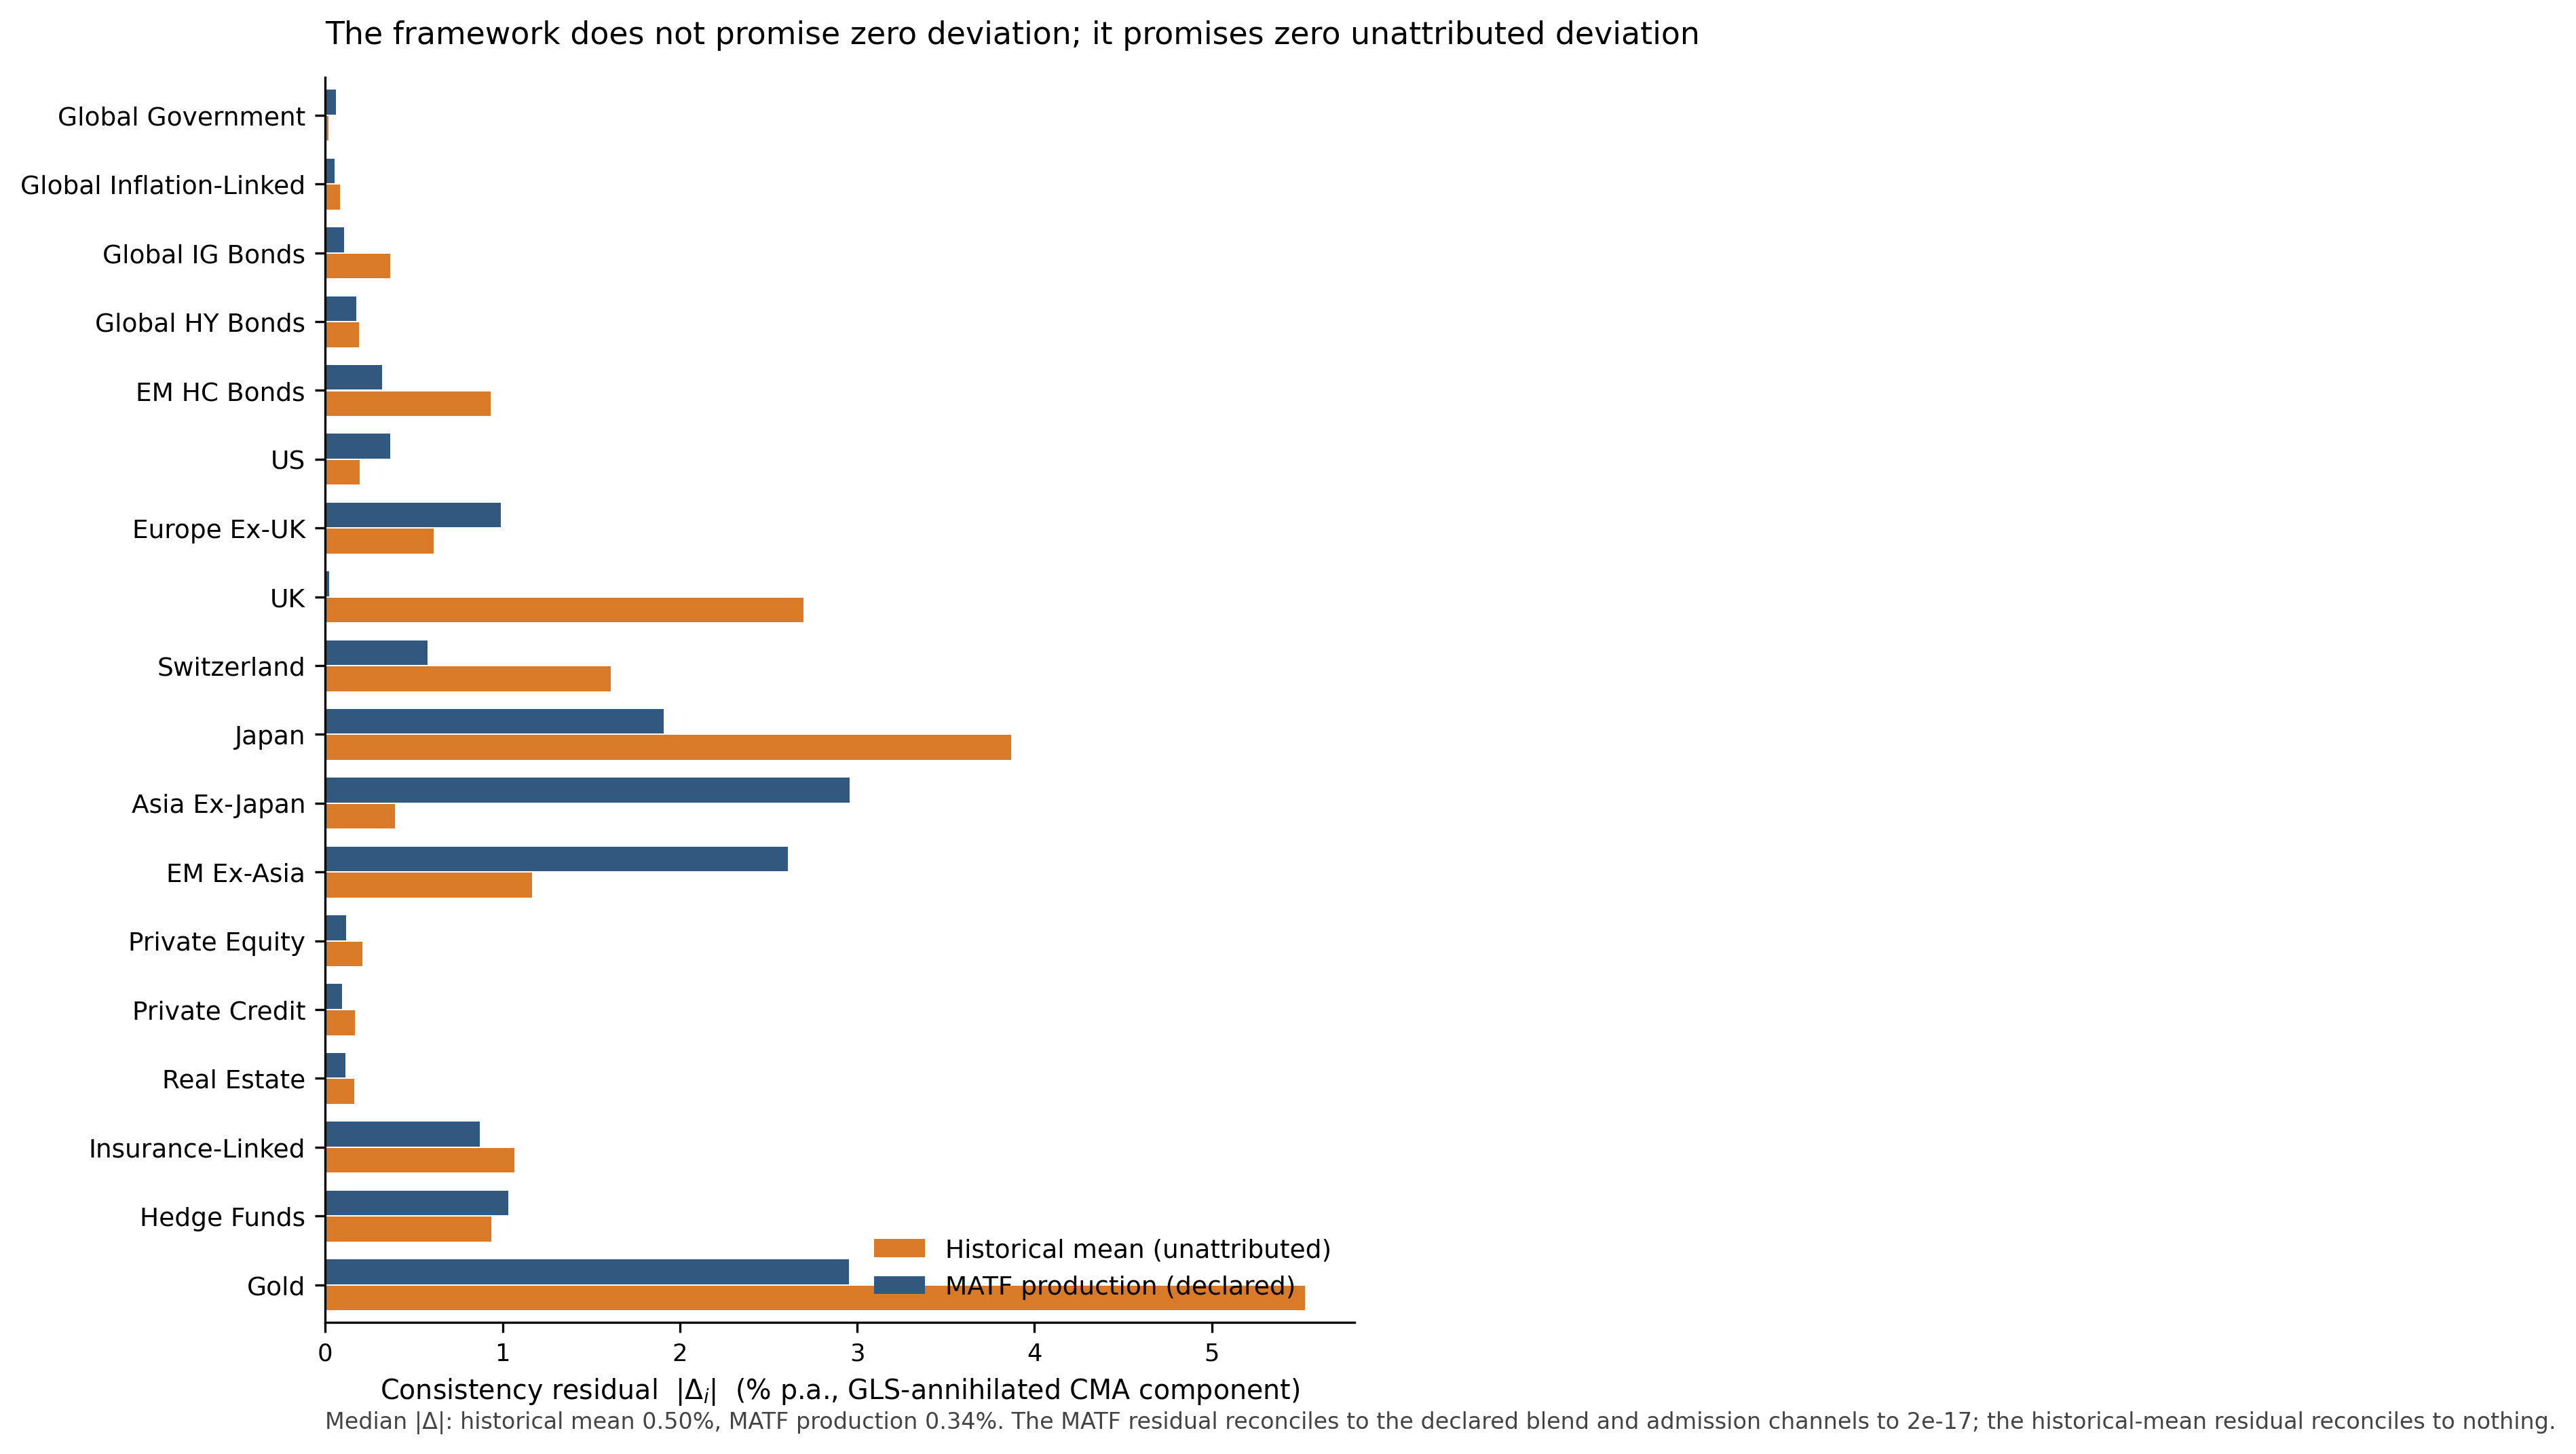
\includegraphics[width=0.85\linewidth]{figures/declared_delta.PNG}
		\end{center}
		\vspace*{-1.0\baselineskip}
		{\footnotesize Notes: per-asset consistency residual $|\Delta_i|$ on the 2026-Q2 cut, USD, identical loadings and residual variances for both constructions. Orange: per-asset historical-mean CMAs, whose residual reconciles to nothing. Blue: MATF production CMAs, whose residual reconciles to the declared blend and admission channels to numerical precision. The bootstrap sampling-distribution version appears in Appendix~B.}
	\end{figure}
	
	The two audits give the committee its calibration in two numbers. The expected-return surface it approves carries half the sampling bandwidth of a per-asset construction on the same record, and every deviation of that surface from the factor model reconciles exactly to a decision the committee itself has made.
	
	% ===== END section6_trust.tex =====
	
	% ===== BEGIN section7_practice_conclusion.tex =====
	% ======================================================================
	% SECTION 7 — IMPLICATIONS FOR PRACTICE + CONCLUSION
	% Drop-in for the R2 inverted structure. Template: cma_paper_v4.tex.
	% Source: v4 "Implications for Practice" + "Conclusion" (lines 1208-1262),
	% rewritten around the three decisions and the audit loop. The scenario-
	% coherence paragraph of v4 is absorbed by Section 5 and reduced to one
	% sentence here. All numbers are the frozen 2026-Q2 values, bootstrap
	% numbers from run_bootstrap_q2.py (B = 500).
	% ======================================================================
	
	\sectionfont{\MakeUppercase}
	\section*{Implications for Practice}\label{sec:practice}
	
	The framework changes what an Investment Committee debates. Under per-asset construction, CMA review is a negotiation over dozens of correlated component forecasts, with cross-asset consistency maintained informally and stress cases specified asset by asset. Under MATF-CMA, the review reduces to a small set of controls that are explicit, separated, and auditable from the published workbook.
	
	\paragraph*{The Control Inventory.} Practitioner judgment concentrates in six controls. The nine factor Sharpe ratios set the premia of Exhibit~\ref{tab:nine_factors}. The prior dispersion $\sigma_{SR}$ sets how tightly the premia anchor to their long-run levels in the uncertainty analysis. The sign constraints of Exhibit~\ref{tab:sign_constraints} encode the economic priors of the loading matrix. The three declared adjustment channels of Equation~\eqref{eq:cma2a} govern every deviation from the factor model, with the admission weights $w_i \in [0,1]$ bounded by the two caps of Exhibit~\ref{tab:admission_audit}. The scenario vectors $\Delta\boldsymbol\lambda$ define stress and upside cases in nine numbers each. Every other object, including loadings, residual variances, and asset-level CMAs, is mechanical. The controls close an audit loop: the waterfall of Exhibit~\ref{fig:construction_waterfall} shows what was decided, the caps test whether the admissions stay within policy, and the reconciliation of Section ``How Much to Trust the Numbers'' verifies that nothing else entered.
	
	\paragraph*{Cross-Currency Deployment.} Institutions running mandates in several base currencies typically maintain parallel CMA systems with separate inflation and FX forecasts per region. The excess-return construction removes the duplication. An asset's excess return over local cash equals its hedged excess return over any other currency's cash up to the cross-currency basis, so all currency panels share the same factor premia. No explicit inflation forecast is required, because regional inflation is embedded in the local risk-free rate through the Fisher relation. A single CMA process therefore produces parallel panels for every operating currency, with currency-specific inputs limited to the local rate curve and the hedging basis. Appendix~D develops the construction.
	
	\paragraph*{Migrating an Existing Process.} The consistency diagnostic of Appendix~A is the natural entry point. Applied to the incumbent CMA vector and risk model, it returns one scalar: the baseline magnitude of unattributed deviation in the current optimization, directly comparable to the $3.4\%$ median norm measured for the sample-mean construction in Section ``How Much to Trust the Numbers''. Three migration paths then cover the common methodologies. A Grinold-Kroner process replaces four component forecasts per asset with nine factor Sharpe ratios and estimated loadings. A qualitative factor mapping replaces hand-set factor weights with estimated loadings while keeping the committee's debate over factor views. A Black-Litterman process replaces the market-cap equilibrium prior with $\hat{\boldsymbol\beta}\boldsymbol\lambda$ and restates views in factor space, which removes the view-uncertainty matrix as a calibration object \citep{RoncalliXu2024}. Migration need not be atomic: an institution can adopt the factor structure and loadings first, retain its premium views, and shift the premium calibration to the market-implied channels as confidence grows.
	
	\sectionfont{\MakeUppercase}
	\section*{Conclusion}\label{sec:conclusion}
	
	We developed the MATF-CMA framework, in which every asset's expected return is its loading on nine tradable factors times market-implied factor premia, plus three declared adjustment channels logged per asset. The same loading matrix defines the covariance model, so consistency between expected returns and risk is a reconciliation the replication code verifies, not a property the practitioner asserts. We organized the empirical analysis around the three decisions an allocation committee takes when it adopts a CMA set, on a production 18-asset universe at the 2026-Q2 cut.
	
	The quantified results are as follows. On the provider decision, five CMA sets optimized on a common risk model, benchmark, and constraints produced Balanced-mandate expected returns from $7.9\%$ to $11.3\%$ and excess Sharpe ratios from $0.35$ to $0.67$ on nearly identical portfolios. The provider choice is therefore a pure expected-return disagreement that the framework prices and attributes. On the admission decision, scaling the alternatives' admitted alpha from zero to the production policy lifted the claimed Sharpe ratio from $0.30$ to $0.35$ with almost no change in weights. Removing the mandate guardrails let the production admission place $78\%$ of the book in alternatives. The raw admissions claimed an idiosyncratic squared Sharpe of $1.40$ against a factor opportunity set of $0.57$, of which $0.63$ survived the premium projection of the companion paper. The two proposed caps flagged the sleeves carrying the excess, including the private-equity admission that we recut from full to half weight. On the scenario decision, one nine-element shock vector repriced every asset and mandate. The admission interaction is explicit: the Balanced stress case flipped sign from $-0.3\%$ to $+0.3\%$ between zero and production admission, because admitted alpha does not shock. On calibration, the factor structure with an economic prior halved the $90\%$ sampling bandwidth of the long-only frontier, equivalent to roughly four times the historical sample. Per-asset construction left unattributed residuals with per-asset medians of $30$ to $115$ basis points and a median portfolio norm of $3.4\%$, against exact reconciliation to the declared channels under MATF.
	
	Two extensions lie outside this paper. The Sharpe-ratio accounting that prices admissions and universe selection in closed form is developed in the companion paper \citep{SeppKastenholzFAJ2026}. The private-equity extension, which replaces appraisal-based loading estimates with cash-flow-based ones and would shrink the statistical alpha the admission policy must govern, is deferred to future work.
	
	\sectionfont{\MakeUppercase}
	\section*{Acknowledgments}
	We thank Ivan Ossa and Rohit Ahluwalia for their constructive discussions and feedback.
	
	% ===== END section7_practice_conclusion.tex =====
	
	\newpage
	\sectionfont{\MakeUppercase}
	\section*{Appendices}\label{sec:appendices}
	% ===== BEGIN appendix_a.tex =====
	% Appendix A: consistency diagnostic (v4 1271-1344) + framework comparison (v4 308-397).
	% R2 changes: declared-channels generalisation of eq:delta_with_alpha, w in [0,1].
	\subsection*{Appendix A: The Alpha-Beta Consistency Diagnostic}\label{app:consistency_diagnostic}
	
	This appendix develops the orthogonal-projection consistency diagnostic referenced in Section ``How Much to Trust the Numbers'' in general form, independent of how the CMA vector or the factor loading matrix is constructed. The underlying operator is the standard factor-model pricing-error projection of \cite{Ross1976} and \cite{Cochrane2005}, repurposed here as a forward-looking coherence check between a practitioner-specified $\boldsymbol\mu$ and the factor loading matrix $\hat{\boldsymbol\beta}$ used in the same allocation problem.
	
	\paragraph*{General Form of the Diagnostic.}
	
	Given any factor loading matrix $\boldsymbol\beta \in \mathbb{R}^{N\times M}$ of full column rank, define the orthogonal projector onto its column space and its complement:
	\begin{equation}\label{eq:projectors}
		\boldsymbol P_\beta = \boldsymbol\beta(\boldsymbol\beta^\intercal\boldsymbol\beta)^{-1}\boldsymbol\beta^\intercal, \qquad \boldsymbol M_\beta = \boldsymbol I_N - \boldsymbol P_\beta.
	\end{equation}
	Both are idempotent ($\boldsymbol P_\beta^2 = \boldsymbol P_\beta$, $\boldsymbol M_\beta^2 = \boldsymbol M_\beta$) and satisfy the annihilation identity
	\begin{equation}\label{eq:annihilation}
		\boldsymbol M_\beta\,\boldsymbol\beta = \boldsymbol 0,
	\end{equation}
	since each column of $\boldsymbol\beta$ already lies in $\text{col}(\boldsymbol\beta)$ and so $\boldsymbol P_\beta\boldsymbol\beta = \boldsymbol\beta$. For any candidate excess-CMA vector $\boldsymbol\mu - r_f\boldsymbol 1$ and any factor loading matrix $\boldsymbol\beta$, the consistency residual is
	\begin{equation}\label{eq:consistency_residual}
		\boldsymbol\Delta(\boldsymbol\mu, \boldsymbol\beta) = \boldsymbol M_\beta\,(\boldsymbol\mu - r_f\boldsymbol 1) = \big(\boldsymbol I - \boldsymbol\beta(\boldsymbol\beta^\intercal\boldsymbol\beta)^{-1}\boldsymbol\beta^\intercal\big)(\boldsymbol\mu - r_f\boldsymbol 1).
	\end{equation}
	The consistency error $\|\boldsymbol\Delta\|_2$ measures the portfolio-level alpha-beta inconsistency, and $|\Delta_i|$ measures the per-asset inconsistency on asset $i$. The protocol requires only the CMA vector and the loading matrix and is independent of how either was constructed, providing a directly comparable metric across CMA methodologies and factor risk models.
	
	\paragraph*{MATF-CMA Delivers $\boldsymbol\Delta \equiv \boldsymbol 0$ by Construction.}
	
	Under the MATF-CMA specification, the excess CMA vector is constructed as
	\begin{equation}\label{eq:matf_construction}
		\boldsymbol\mu^{MATF} - r_f\boldsymbol 1 = \hat{\boldsymbol\beta}\,\boldsymbol\lambda^{MATF},
	\end{equation}
	where $\boldsymbol\lambda^{MATF} \in \mathbb{R}^M$ is the factor risk-premium vector and $\hat{\boldsymbol\beta}$ is the same estimated loading matrix that defines the asset covariance $\boldsymbol\Sigma = \hat{\boldsymbol\beta}\boldsymbol\Sigma_F\hat{\boldsymbol\beta}^\intercal + \boldsymbol D_\varepsilon$. Substituting Equation~\eqref{eq:matf_construction} into the diagnostic~\eqref{eq:consistency_residual} and applying the annihilation identity~\eqref{eq:annihilation}:
	\begin{equation}\label{eq:matf_zero}
		\boldsymbol\Delta^{MATF} = \boldsymbol M_{\hat\beta}\,\hat{\boldsymbol\beta}\,\boldsymbol\lambda^{MATF} = \boldsymbol 0.
	\end{equation}
	The residual vanishes by virtue of the structural form $\boldsymbol\mu^{MATF} - r_f\boldsymbol 1 \in \text{col}(\hat{\boldsymbol\beta})$, not by virtue of any specific calibration of $\boldsymbol\lambda^{MATF}$. The identity holds for every $\boldsymbol\lambda^{MATF}$, every bootstrap draw, and every data-independent perturbation of the inputs.
	
	The production MATF specification extends Equation~\eqref{eq:matf_construction} with the three declared adjustment channels of Equation~\eqref{eq:cma2a}: $\boldsymbol\mu - r_f\boldsymbol 1 = \hat{\boldsymbol\beta}\boldsymbol\lambda + \boldsymbol b + \boldsymbol W\boldsymbol\alpha + \boldsymbol a$, where $\boldsymbol b$ is the regional valuation blend, $\boldsymbol W = \text{diag}(w_1,\dots,w_N)$ with $w_i \in [0,1]$ the admission weights on statistical alphas, and $\boldsymbol a$ the gross add-on. In that case
	\begin{equation}\label{eq:delta_with_alpha}
		\boldsymbol\Delta = \boldsymbol M_{\hat\beta}\,(\boldsymbol b + \boldsymbol W\boldsymbol\alpha + \boldsymbol a),
	\end{equation}
	which equals $\boldsymbol 0$ when no adjustments are declared and otherwise equals the orthogonal-complement projection of the declared adjustment vector. The residual therefore reflects only intentional, logged deviations from the factor model, never unattributed artifacts, and the reconciliation of Equation~\eqref{eq:delta_with_alpha} against the published workbook is asserted by the replication code at each production cut.
	
	
	
	\paragraph*{Applying the Diagnostic to Black-Litterman.}
	
	The standard Black-Litterman construction \citep{BlackLitterman1992} combines an equilibrium excess-return prior with a set of $K$ linear views on asset returns:
	\begin{equation}\label{eq:bl_construction}
		\boldsymbol\Pi = \delta\boldsymbol\Sigma\boldsymbol w_{mkt}, \qquad
		\boldsymbol\mu^{BL} = \boldsymbol\Pi + \tau\boldsymbol\Sigma\boldsymbol P^\intercal\big(\boldsymbol P\tau\boldsymbol\Sigma\boldsymbol P^\intercal + \boldsymbol\Omega\big)^{-1}\big(\boldsymbol Q - \boldsymbol P\boldsymbol\Pi\big),
	\end{equation}
	where $\boldsymbol P \in \mathbb{R}^{K \times N}$ is the view picking matrix, $\boldsymbol Q \in \mathbb{R}^K$ contains view values, $\boldsymbol\Omega \in \mathbb{R}^{K \times K}$ is the view-uncertainty matrix, $\boldsymbol w_{mkt} \in \mathbb{R}^N$ are market-cap weights, $\delta$ is risk aversion, and $\tau$ is prior confidence. We decompose the covariance into systematic and idiosyncratic components, $\boldsymbol\Sigma = \hat{\boldsymbol\beta}\boldsymbol\Sigma_F\hat{\boldsymbol\beta}^\intercal + \boldsymbol D_\varepsilon$, and apply the annihilation identity~\eqref{eq:annihilation}
	\begin{equation}\label{eq:msigma_identity}
		\boldsymbol M_{\hat\beta}\boldsymbol\Sigma = \boldsymbol M_{\hat\beta}\hat{\boldsymbol\beta}\boldsymbol\Sigma_F\hat{\boldsymbol\beta}^\intercal + \boldsymbol M_{\hat\beta}\boldsymbol D_\varepsilon = \boldsymbol M_{\hat\beta}\boldsymbol D_\varepsilon,
	\end{equation}
	since the systematic block is annihilated. Substituting Equation~\eqref{eq:bl_construction} into the diagnostic~\eqref{eq:consistency_residual} and applying Equation~\eqref{eq:msigma_identity} yields:
	\begin{equation}\label{eq:bl_delta}
		\boldsymbol\Delta^{BL} = \boldsymbol M_{\hat\beta}\boldsymbol D_\varepsilon\big(\delta\boldsymbol w_{mkt} + \tau\boldsymbol P^\intercal\boldsymbol c\big),
		\qquad \boldsymbol c = \big(\boldsymbol P\tau\boldsymbol\Sigma\boldsymbol P^\intercal + \boldsymbol\Omega\big)^{-1}\big(\boldsymbol Q - \boldsymbol P\boldsymbol\Pi\big).
	\end{equation}
	The residual decomposes into a prior contribution $\delta\boldsymbol M_{\hat\beta}\boldsymbol D_\varepsilon\boldsymbol w_{mkt}$, sourced from the idiosyncratic-variance component of the equilibrium prior, and a view contribution $\tau\boldsymbol M_{\hat\beta}\boldsymbol D_\varepsilon\boldsymbol P^\intercal\boldsymbol c$, sourced from how views interact with the residual variance. The prior contribution is small for traditional asset universes with concentrated market weights and low residual variance, but non-trivial for any universe containing alternatives. The view contribution is generically non-zero because the view design $(\boldsymbol P, \boldsymbol Q, \boldsymbol\Omega)$ carries no constraint requiring $\boldsymbol P^\intercal\boldsymbol c \in \text{col}(\hat{\boldsymbol\beta})$. Therefore $\boldsymbol\Delta^{BL} = \boldsymbol 0$ only when $\boldsymbol D_\varepsilon\big(\delta\boldsymbol w_{mkt} + \tau\boldsymbol P^\intercal\boldsymbol c\big) \in \text{col}(\hat{\boldsymbol\beta})$ --- a non-generic algebraic coincidence that holds trivially when $\boldsymbol D_\varepsilon = \boldsymbol 0$ (covariance is fully factor-structured with no idiosyncratic variance) and otherwise fails for almost any choice of view design. 
	
	The factor-space reformulation of \citet{RoncalliXu2024} restores consistency by relocating the judgment from $N$-dimensional asset return space to $M$-dimensional factor premium space. With views specified on factor premia and the asset CMA constructed as $\boldsymbol\mu^{factor\text{-}BL} - r_f\boldsymbol 1 = \hat{\boldsymbol\beta}\boldsymbol\lambda^{BL}$, the annihilation identity~\eqref{eq:annihilation} delivers $\boldsymbol\Delta^{factor\text{-}BL} = \boldsymbol 0$
	identically.
	
	
	\paragraph*{Diagnostic Without an Explicit Factor Model.}
	
	The protocol does not require the practitioner to commit to a named factor model. When only a generic covariance matrix $\boldsymbol\Sigma$ is available --- for example, from a commercial risk model whose internal factor parameterization is proprietary --- the loading matrix can be extracted as the top-$M$ principal components of $\boldsymbol\Sigma$. Letting $\boldsymbol\Sigma = \boldsymbol U\boldsymbol\Lambda\boldsymbol U^\intercal$ with eigenvalues in decreasing order and some rank $M$ chosen to capture a target fraction of variance, we set the beta loading and diagnostic as follows:
	\begin{equation}\label{eq:pca}
		\hat{\boldsymbol\beta}_{PCA} = \boldsymbol U_M\boldsymbol\Lambda_M^{1/2}, \quad \boldsymbol\Delta = \boldsymbol M_{\hat\beta_{PCA}}(\boldsymbol\mu - r_f\boldsymbol 1)
	\end{equation}
	The projection operator $\boldsymbol M_{\hat\beta_{PCA}}$ defined as in Equation~\eqref{eq:projectors} then measures inconsistency between the CMA vector and the implicit statistical factor structure of $\boldsymbol\Sigma$. The value of consistency residual norm $\|\boldsymbol\Delta\|_2$ is invariant under rotations of $\boldsymbol U_M$, so the diagnostic is well-defined even though per-PC labels are not. This extension makes the protocol applicable to any practitioner risk model regardless of its native parameterization, and provides a route to cross-method comparison when factor specifications differ.
	
	\paragraph*{Relation to the Asset Pricing Literature.}
	The operator $\boldsymbol M_\beta$ in Equation~\eqref{eq:projectors} is the workhorse of classical factor-model pricing-error tests. \cite{Ross1976} establishes that the Arbitrage Pricing Theory predicts $\mathbb{E}[\boldsymbol R^e] \in \text{col}(\boldsymbol\beta)$, so $\boldsymbol M_\beta\mathbb{E}[\boldsymbol R^e]$ measures the APT pricing error by construction. \cite{Cochrane2005}, ch.~12, develops $\boldsymbol\alpha = \boldsymbol\mu - \boldsymbol\beta\boldsymbol\lambda$ as the standard model pricing error in a stochastic-discount-factor framework.
	
	
	
	\paragraph*{Comparison of CMA Construction Frameworks.}
	Exhibit~\ref{tb:framework_comparison} compares four CMA construction methodologies --- per-asset Grinold-Kroner, standard Black-Litterman, the factor-Black-Litterman reformulation of \citet{RoncalliXu2024}, and the MATF-CMA framework of this paper --- across the inputs an Investment Committee must provide and the structural properties of the result.
	
	The four approaches differ less in the count of judgment inputs than in their nature. Per-asset GK requires $\sim 4N$--$6N$ component forecasts per asset. The BL variants reduce this to a handful of views plus an equilibrium prior and a view-uncertainty matrix whose calibration lacks an external benchmark. MATF-CMA shifts judgment to $M$ direct factor-premium calibrations, each anchored to an independent sub-asset-class evidence channel.
	
	Per-asset GK and standard BL produce $\boldsymbol\Delta \neq \boldsymbol 0$ generically. Factor-BL and MATF-CMA both achieve $\boldsymbol\Delta \equiv \boldsymbol 0$ when no adjustments are declared, by the structural identity $\boldsymbol\mu - r_f\boldsymbol 1 \in \text{col}(\hat{\boldsymbol\beta})$. MATF additionally accommodates declared deviations through the channels of Equation~\eqref{eq:delta_with_alpha}, a mechanism factor-BL lacks.
	
	Factor-BL and MATF-CMA are complementary: factor-BL is a Bayesian update on $\boldsymbol\lambda$ that requires a prior, and MATF-CMA produces one. An institution wishing to apply Bayesian shrinkage to tactical factor views can set $\boldsymbol\lambda^\Pi := \boldsymbol\lambda^{MATF}$ and inherit both.
	
	\begin{table}[H]
		\caption{Comparison of Four CMA Construction Frameworks}\label{tb:framework_comparison}\vspace*{-0.5\baselineskip}
		\centering
		\footnotesize
		\renewcommand{\arraystretch}{1.15}
		\begin{tabular}{p{0.20\textwidth} p{0.18\textwidth} p{0.18\textwidth} p{0.18\textwidth} p{0.18\textwidth}}
			\hline
			& \textbf{Per-asset GK} & \textbf{Standard BL} & \textbf{Factor-BL} & \textbf{MATF-CMA} \\
			& \citep{GrinoldKroner2002} & \citep{BlackLitterman1992} & \citep{RoncalliXu2024} & this paper \\
			\hline
			Output $\boldsymbol\mu$ & 
			Bottom-up per asset from yield, growth, valuation reversion components & 
			Bayesian posterior $\boldsymbol\mu^{BL}$ from prior $\boldsymbol\Pi$ + views & 
			$\boldsymbol\mu^{BL} = \hat{\boldsymbol\beta}\boldsymbol\lambda^{BL}$ from factor-space posterior & 
			$\boldsymbol\mu^{MATF} = \hat{\boldsymbol\beta}\boldsymbol\lambda^{MATF} + \boldsymbol W\boldsymbol\alpha$ from direct calibration \\
			\hline
			\multicolumn{5}{l}{\textit{Estimated objects (data-driven; judgment-light)}} \\
			\hline
			Covariance & 
			Risk model (external) $\boldsymbol\Sigma$ & 
			$\boldsymbol\Sigma$ (typically historical) & 
			$\boldsymbol\Sigma_F$ on $M$ factors & 
			$\boldsymbol\Sigma_F$ on $M$ factors \\
			Factor loadings $\hat{\boldsymbol\beta}$ & 
			--- & 
			--- (or for risk only) & 
			Required, estimator unspecified & 
			HCGL with sign and cluster-prior constraints \\
			\hline
			\multicolumn{5}{l}{\textit{Judgment inputs the Investment Committee must provide}} \\
			\hline
			Premium / view specification & 
			$\sim 4\text{--}6$ component forecasts per asset $\rightarrow \sim 4N\text{--}6N$ inputs & 
			$K$ asset-space views $(\boldsymbol P, \boldsymbol Q) \in \mathbb{R}^{K \times N} \times \mathbb{R}^K$ & 
			$K^F$ factor-space views $(\boldsymbol P^F, \boldsymbol Q^F) \in \mathbb{R}^{K^F \times M} \times \mathbb{R}^{K^F}$ & 
			Direct calibration of $M$ factor premia from independent evidence channels \\
			Equilibrium prior & 
			None (point forecasts) & 
			$\boldsymbol\Pi = \delta\boldsymbol\Sigma\boldsymbol w_{mkt}$; requires $\boldsymbol w_{mkt}$ (problematic for alternatives) and $\delta$ & 
			$\boldsymbol\lambda^\Pi \in \mathbb{R}^M$; sourcing unspecified (reverse-optimization, history, or theory) & 
			None; premia calibrated directly \\
			View uncertainty & 
			--- & 
			$\boldsymbol\Omega \in \mathbb{R}^{K \times K}$ (typically diagonal); elicitation acknowledged as the operational pain point of BL & 
			$\boldsymbol\Omega^F \in \mathbb{R}^{K^F \times K^F}$; same elicitation problem in factor space & 
			--- (no posterior update) \\
			Prior confidence $\tau$ & 
			--- & 
			Required scalar & 
			Required scalar & 
			--- \\
			Explicit alpha admission & 
			Implicit in per-asset components & 
			Implicit in views & 
			None natively & 
			$\boldsymbol W\boldsymbol\alpha$, with $\boldsymbol W = \mathrm{diag}(w_i)$, $w_i \in \{0,1\}$ \\
			\hline
			\multicolumn{5}{l}{\textit{Structural properties}} \\
			\hline
			Equilibrium anchor & None & Asset-space reverse-optimization & Factor-space reverse-optimization or theory & Per-factor sub-asset-class evidence channels$^{b}$ \\
			Tactical layer & Embedded in per-asset components & Embedded in $\boldsymbol Q$ & Embedded in $\boldsymbol Q^F$ & Separated (ROSAA-TAA, \citealp{Rosaa2026}) \\
			Consistency residual $\boldsymbol\Delta = \boldsymbol M_{\hat\beta}(\boldsymbol\mu - r_f\boldsymbol 1)$ & 
			Large; $\boldsymbol\Delta \neq \boldsymbol 0$ generically & 
			$\boldsymbol\Delta^{BL} \neq \boldsymbol 0$; prior pulls toward $\text{col}(\hat{\boldsymbol\beta})$ partially via factor-structured $\boldsymbol\Sigma$ but views break it & 
			$\boldsymbol\Delta^{BL} \equiv \boldsymbol 0$ by structural identity $\boldsymbol\mu \in \text{col}(\hat{\boldsymbol\beta})$ & 
			$\boldsymbol\Delta^{MATF} \equiv \boldsymbol M_{\hat\beta}(\boldsymbol b + \boldsymbol W\boldsymbol\alpha + \boldsymbol a)$; zero when no adjustments declared, otherwise the annihilated image of the declared adjustments \\
			\hline
		\end{tabular}
		\begin{flushleft}
			\small
			NOTE: $N$ = number of assets, $M$ = number of factors, $K$ ($K^F$) = number of asset-space (factor-space) views; typically $K, K^F \in [3, 8]$ per cycle while $M \approx 9$ and $N \in [15, 200]$ for multi-asset universes.
		\end{flushleft}
	\end{table}
	
	
	
	
	
	
	\sectionfont{\MakeUppercase}
	
	% ===== END appendix_a.tex =====
	
	% ===== BEGIN appendix_b.tex =====
	% ======================================================================
	% APPENDIX B — BOOTSTRAP DESIGN AND ESTIMATION-ERROR ANALYSIS
	% Source: v4 App B (1346-1409) + the unified SE comparison moved from the
	% v4 bootstrap section (1122-1156) + the GK variance equation (v4 175).
	% Q2 updates: 18 assets (14 ME + 4 QE), window Jul 2001 - Jun 2026,
	% SR prior [0.35,0.35,0.25,0.25,0.15,0.15,0.50,0.25,0.00], backfills
	% EHFI804 <- HFRIFWI and MSDEXKSN <- MSDEE15N, log-return panel with
	% arithmetic lift. SE triple recomputed on Q2 inputs (NDDUUS vol 16.2%,
	% beta_Eq 0.99, sigma_F,Eq 15.4%). Sensitivity table regenerated by
	% run_sensitivity_q2.py (values patched from figures/sr_sensitivity_q2.csv).
	% ======================================================================
	
	\subsection*{Appendix B: Bootstrap Design and Estimation-Error Analysis}\label{subsec:bootstrap_design}
	
	We compare two estimators of the long-only mean-variance efficient frontier on the 18-asset universe of the main text, comprising 14 monthly-frequency assets and 4 quarterly-frequency alternatives, over a $300$-month window from July 2001 to June 2026. Two short-history sleeves are backfilled with pre-inception proxies at unit scale: the Eurekahedge insurance-linked index with the hedge-fund index through June 2006, and the Europe ex-UK equity index with the broad Europe index through October 2007. The full procedure, including design-choice rationale and implementation details, is documented in the supplementary code repository \citep{MatfCmaCode2026}.
	
	\textbf{1) Raw asset-level estimator:} Each bootstrap draw computes the sample mean and pairwise-complete sample covariance of resampled asset returns, then solves the long-only frontier on a vol-target grid. The panel is stored in native-frequency excess log returns, so per-asset means carry the arithmetic lift of one half the variance. This estimator is mathematically identical to a Grinold-Kroner construction in which the per-asset point estimate is the historical sample mean.
	
	\textbf{2) MATF factor-structured estimator:} Each bootstrap draw resamples paired factor return and asset residual panels, re-estimates the factor covariance $\Sigma_F$ and the residual variance vector $D$, draws factor risk premia $\boldsymbol\lambda$ from a structural Sharpe-ratio prior, and reconstructs the asset moments as
	\begin{equation}
		\boldsymbol\mu = r_f + \hat{\boldsymbol\beta}\boldsymbol\lambda, \ \Sigma = \hat{\boldsymbol\beta}\,\Sigma_F\,\hat{\boldsymbol\beta}^{\intercal} + D
	\end{equation}
	using the same estimated factor loading matrix $\hat{\boldsymbol\beta}$ as the rest of the framework.
	
	We use the stationary block bootstrap of \cite{PolitisRomano1994} with mean block length $L = 12$ months and minimum block length $L_{\min} = 3$ months to preserve quarterly observations within each block. We assume that the Sharpe-ratio prior is multivariate normal:
	\begin{equation}\label{eq:matf_sharpe}
		\mathrm{SR}^{(b)} \sim \mathcal{N}(\boldsymbol{m}_{\mathrm{SR}}, \Sigma_{\mathrm{SR}})
	\end{equation}
	with mean vector $\boldsymbol{m}_{\mathrm{SR}} = (0.35, 0.35, 0.25, 0.25, 0.15, 0.15, 0.50, 0.25, 0.00)$ in the order (Equity, Rates, Credit, Carry, Inflation, Commodities, Private Equity, Rates Volatility, FX), the production prior vector of the 2026-Q2 cut. The Equity, Rates, and Credit entries are the long-run averages of the respective factor premia divided by their volatility targets. Cross-factor correlations are set to those of the factor covariance $\Sigma_F$, and we use a constant per-factor standard deviation $\sigma_{\mathrm{SR}}$ so that $\Sigma_{\mathrm{SR}} = \sigma_{\mathrm{SR}}^2\,\rho_F$ with $\rho_F$ the factor correlation matrix.
	
	We set $\sigma_{\mathrm{SR}} = 0.10$ because at the effective sample size $T_{\mathrm{eff}} \approx 25$, the sample-mean Sharpe-ratio estimator has asymptotic standard deviation $1/\sqrt{T_{\mathrm{eff}}} \approx 0.20$ \citep{Lo2002}. The value $\sigma_{\mathrm{SR}} = 0.10$ therefore encodes a prior twice as tight as the historical record, informationally equivalent to four times the sample size. The implied $95\%$ prior interval of $\pm 0.20$ around each factor's mean spans the dispersion of point estimates across published cross-asset Sharpe-ratio surveys. For example, an equity SR in $[0.15, 0.55]$ aligns with the standard $4\%$--$8\%$ equity-premium range \citep{Ilmanen2011}, and a PE SR in $[0.30, 0.70]$ covers the illiquidity-premium debate.
	
	\paragraph*{Robustness of the MATF Reduction Ratio to $\sigma_{\mathrm{SR}}$.}
	
	We test the robustness of the $2\times$ reduction reported in Section ``How Much to Trust the Numbers'' by re-running the bootstrap at six $\sigma_{\mathrm{SR}}$ values, reported in Exhibit~\ref{tab:sr_sensitivity}.
	
	\begin{table}[H]
		\captionof{table}{Sensitivity of the MATF Reduction Ratio to the SR-Prior Dispersion $\sigma_{\mathrm{SR}}$}\label{tab:sr_sensitivity}\vspace*{-1.0\baselineskip}
		\begin{center}
			\small
			\begin{tabular}{cccl}
				\toprule
				$\sigma_{\mathrm{SR}}$ & Reduction ratio & $T_{\mathrm{eff}}$ equivalent & Regime \\
				\midrule
				0.050 & 3.83$\times$  & 14.7$\times$ & Aggressive prior \\
				0.075 & 2.57$\times$  & 6.6$\times$ & Moderate--aggressive \\
				\textbf{0.100} & \textbf{2.01$\times$}  & \textbf{4.0$\times$} & \textbf{Paper baseline} \\
				0.125 & 1.62$\times$  & 2.6$\times$ & Moderate--loose \\
				0.150 & 1.41$\times$  & 2.0$\times$ & Loose \\
				0.200 & 1.10$\times$  & 1.2$\times$ & Prior equals data noise scale \\
				\bottomrule
			\end{tabular}
		\end{center}\vspace*{-0.75\baselineskip}
		\small
		NOTE: Bootstrap reduction ratio of the 90\% efficient-frontier bandwidth for the MATF estimator at the Balanced w/o-Alts target volatility of $9.3\%$, across the SR-prior dispersion grid. Each row is a separate $B = 500$ bootstrap replication on the $300$-month window of the 2026-Q2 cut; only $\sigma_{\mathrm{SR}}$ varies. The $T_{\mathrm{eff}}$ equivalent is the squared reduction ratio, representing the additional historical sample size to which the MATF prior is informationally equivalent.
	\end{table}\vspace*{-0.75\baselineskip}
	
	Three properties follow. The qualitative finding holds across $\sigma_{\mathrm{SR}} \in [0.05, 0.15]$ with reduction ratios between $1.4\times$ and $3.8\times$. The limit $\sigma_{\mathrm{SR}} = 0.20$ approaches the sample-mean bandwidth, because a prior as wide as the data adds no information. The $T_{\mathrm{eff}}$ multiplier scales as $1/\sigma_{\mathrm{SR}}^2$, consistent with Gaussian-prior intuition.
	
	\paragraph*{Estimation Error: A Unified Comparison.}
	
	Each of the three CMA methodologies, the historical sample mean, Grinold-Kroner building blocks, and MATF-CMA, writes the expected return $\hat R_i$ as a linear function of an estimated input vector $\boldsymbol{\hat\theta}$. The standard error of $\hat R_i$ then follows from the variance of a linear form,
	\begin{equation}\label{eq:var_gk}
		\operatorname{Var}(\hat{R}) = \sum_i \operatorname{Var}(\hat{\theta}_i) + 2\sum_{i<j} \operatorname{Cov}(\hat{\theta}_i, \hat{\theta}_j),
	\end{equation}
	and the three methodologies differ in the dimension of $\boldsymbol{\hat\theta}$, the source of dispersion, and whether the variance shrinks with the sample or with cross-asset pooling.
	
	The sample-mean estimator uses $T_{\mathrm{eff}} = T/L \approx 25$ effectively independent annual observations, giving the standard error $\sigma_i / \sqrt{T_{\mathrm{eff}}}$, which equals $3.2\%$ for US equity at the Q2 volatility of $16.2\%$. The Grinold-Kroner construction sums four component forecasts per asset. With realistic component standard errors ($0.1\%$ for the payout yield, $1.5\%$ for real growth, $1.0\%$ for inflation, $2.0\%$ for valuation reversion) and a uniform pairwise correlation of $\rho = 0.5$ reflecting shared macroeconomic drivers, Equation~\eqref{eq:var_gk} gives $3.6\%$ \citep{ChopraZiemba1993}. The GK variance does not shrink with $T$, because each component is a forecast of a separate underlying process.
	
	The MATF estimator writes $\hat R_i = r_f + \hat{\boldsymbol\beta}_i^{\intercal}\hat{\boldsymbol\lambda}$ with $\boldsymbol\lambda = \mathrm{SR} \odot \boldsymbol\sigma_F$. Following \cite{ChopraZiemba1993}, we treat the better-identified loadings and factor volatilities as fixed at leading order and place the remaining randomness in the $M$-dimensional Sharpe-ratio prior of Equation~\eqref{eq:matf_sharpe}. For an asset with exposure concentrated on a single factor $f^\star$, the standard error reduces to
	\begin{equation}\label{eq:se_matf_full}
		\mathrm{SE}(\hat R_i^{MATF}) \approx |\hat\beta_{i, f^\star}| \cdot \sigma_{\mathrm{SR}} \cdot \sigma_{F, f^\star}.
	\end{equation}
	For US equity, with $\hat\beta_{\mathrm{Eq}} = 0.99$, $\sigma_{F,\mathrm{Eq}} = 15.4\%$, and $\sigma_{\mathrm{SR}} = 0.10$, the standard error is $1.5\%$. Exhibit~\ref{tab:se_comparison} summarizes the comparison.
	
	\begin{table}[H]
		\captionof{table}{Standard Error of CMA Estimators for US Equity, 2026-Q2 Inputs}\label{tab:se_comparison}\vspace*{-1.0\baselineskip}
		\begin{center}
			\small
			\begin{tabular}{lccl c}
				\toprule
				\textbf{Estimator} & \textbf{Inputs} & \textbf{Sample size} & \textbf{SE formula} & \textbf{US equity SE} \\
				\midrule
				Sample mean      & $T_{\mathrm{eff}}$ asset returns      & $T/L$ scales noise & $\sigma_i / \sqrt{T_{\mathrm{eff}}}$ & $3.24\%$ \\
				Grinold-Kroner   & $K_{GK} = 4$ forecasts per asset & fixed; no $T$ scaling & Equation~\eqref{eq:var_gk} & $3.64\%$ \\
				MATF-CMA         & $M = 9$ universe-wide factor SRs & cross-asset pooling via $\hat{\boldsymbol\beta}$ & Equation~\eqref{eq:se_matf_full} & $1.53\%$ \\
				\bottomrule
			\end{tabular}
		\end{center}
		\small
		NOTE: Specification: $\sigma_i = 16.2\%$ (NDDUUS, 2026-Q2 cut), $T_{\mathrm{eff}} = 25$, $K_{GK} = 4$ components with $\rho = 0.5$, $M = 9$ MATF factors with $\sigma_{\mathrm{SR}} = 0.10$, $\hat\beta_{\mathrm{Eq}} = 0.99$, $\sigma_{F,\mathrm{Eq}} = 15.4\%$. The three estimators deliver standard errors in the ratio $3.2 : 3.6 : 1.5$, and the bootstrap of the main text confirms the implied ratio of roughly $2{:}1$ between the non-factor methods and MATF.
	\end{table}
	
	% ===== END appendix_b.tex =====
	
	% ===== BEGIN appendix_c.tex =====
	% Appendix C: premium estimation (v4 606-822) + illustrations (v4 869-1002), near-verbatim.
	% [TODO] Regenerate Appendix C figures on the Q2 cut via figures.py (regional P-CAEY,
	% rates CMAs, universe CMA exhibits reference the v4 ArticleFigures files).
	\subsection*{Appendix C: Estimation of the Factor Risk Premia}\label{app:premia}
	
	We now consider the estimation of risk premia for MATF. For equity, rates, and credit factors we develop fundamental data-driven valuation models, while for the remaining structural factors we use an equilibrium-based approach.
	
	
	
	\paragraph*{Equity Factor Risk Premium.}\label{sec:equity}
	
	The equity factor is the dominant driver of expected returns for most multi-asset portfolios. We derive the equity factor risk premium using the Payout and Cyclically-Adjusted Earnings Yield (P-CAEY) methodology of \cite{HaghaniWhite2024}, which improves upon the standard CAPE metric of \cite{CampbellShiller1988}.
	
	The Cyclically-Adjusted Price Earnings ratio (CAPE), Cyclically-Adjusted Earnings (CAE) and Cyclically-Adjusted Earnings Yield (CAEY) are defined as follows:
	\begin{equation}\label{eq:cape}
		\text{CAPE}_t = \frac{P_t}{\text{CAE}_t}, \qquad \text{CAE}_t = \frac{1}{K}\sum_{k=0}^{K-1} \tilde{E}_{t-k}, \qquad \text{CAEY}_t = 1/\text{CAPE}_t
	\end{equation}
	where $P_t$ is the current index price level, $\tilde E_{t-k}$ denotes real earnings per share for year $t-k$ (nominal earnings inflated to date-$t$ prices via the CPI ratio), and $K = 10$ is the smoothing window in years. The CAEY is the reciprocal of CAPE.
	
	CAEY estimates the expected long-term real return under the assumption that companies pay out all earnings and maintain constant real earnings in perpetuity. This assumption is increasingly violated as dividend payout ratios have declined from approximately $65\%$ historically (1880--1988) to around $35\%$ in recent years \citep{HaghaniWhite2024}; standard CAPE treats retained earnings identically to paid-out earnings, ignoring the compounding value of reinvestment and consequently understating expected returns.
	
	\cite{HaghaniWhite2024} propose the Payout and Cyclically-Adjusted Earnings Yield (P-CAEY), which adjusts for retained earnings by compounding the non-dividend portion forward at the prevailing CAEY rate. For each year $s$ in the $K$-year lookback window, the payout-adjusted real earnings are
	\begin{equation}\label{eq:p_adj}
		E_s^{P\text{-}adj} = \underbrace{d_s \cdot \tilde{E}_{s}}_{\text{paid out}} + \underbrace{(1 - d_s) \cdot \tilde{E}_{s} \cdot (1 + \text{CAEY}_s)^{(t - s)}}_{\text{retained, compounded forward}}, \quad  d_s = \text{DPS}_s/\text{EPS}_s \in [0,1]
	\end{equation}
	where $d_s$ is the dividend payout ratio at time $s$ and $\text{CAEY}_s$ is the standard CAEY used as the compounding rate. The P-CAEY is then
	\begin{equation}\label{eq:pcaey_def}
		\text{P-CAEY}_t = \frac{\frac{1}{K}\sum_{k=0}^{K-1} E_{t-k}^{P\text{-}adj}}{P_t}
	\end{equation}
	
	Under the perpetuity assumption, P-CAEY equals the expected long-term real return on equities \citep{HaghaniWhite2024}. The equity factor risk premium is the excess over the real risk-free rate:
	\begin{equation}\label{eq:erp}
		\lambda_{Equity,r} = \text{P-CAEY}_r - r_{f,r}^{real}
	\end{equation}
	Since inflation cancels in this difference between two real quantities, the real excess return equals the nominal excess return. We estimate the real risk-free rate $r_{f,r}^{real}$ using a cascade of decreasing data quality which prioritizes market-implied inflation expectations over backward-looking CPI data:
	\begin{equation}\label{eq:real_rate_cascade}
		r_{f,r}^{real} = \begin{cases}
			y_r^{TIPS} & \text{if inflation-linked bond yield available (US)} \\[3pt]
			r_{f,r}^{10Y,nominal} - \pi_r^{swap,10Y} & \text{if 10Y inflation swap available (Europe, UK)} \\[3pt]
			r_{f,r}^{10Y,nominal} - \pi_r^{breakeven} & \text{if 10Y breakeven available (Japan)} \\[3pt]
			r_{f,r}^{10Y,nominal} - \pi_r^{trailing\,CPI} & \text{otherwise: Fisher fallback}
		\end{cases}
	\end{equation}
	
	
	\subsubsection*{Bottom-Up Global Equity Factor Premium}
	
	The MATF equity factor is constructed from MSCI World futures. Rather than computing P-CAEY directly on the global aggregate, we estimate the global equity factor risk premium via bottom-up aggregation from regional P-CAEYs:
	\begin{equation}\label{eq:global_erp}
		\lambda_{Equity}^{Global} = \sum_{r} w_r \cdot \lambda_{Equity,r}
	\end{equation}
	where $w_r$ are the market-capitalization weights of region $r$ in MSCI World: US 70\%, Eurozone 15\%, Japan 5\%, UK 3\%, Canada 3\%, Switzerland 2.5\%, Australia 1.5\%. Equity indices, CPI series, and government yield tickers per region follow standard Bloomberg conventions; the production configuration is documented in the reproduction code.
	
	Individual regional equity indices are not pure equity exposures. A regional index like the Euro Stoxx 50 is heavily weighted toward energy, industrials, and materials, so its returns co-move with commodity prices, interest rates, and credit spreads in ways that a pure equity factor does not. Pricing European equities using only the European P-CAEY-implied equity risk premium would miss these non-equity return drivers --- a form of the alpha-beta inconsistency the framework is designed to prevent.
	
	The MATF framework decomposes each regional index's return into its constituent factor exposures. The excess CMA for region $r$ is
	\begin{equation}\label{eq:regional_cma}
		\text{CMA}_r^{excess} = \underbrace{\hat{\beta}_r^{eq} \cdot \lambda_{Equity}^{Global} + (1 - \hat{\beta}_r^{eq}) \cdot \lambda_{Equity,r}}_{\text{equity component}} + \underbrace{\sum_{j \neq eq} \hat{\beta}_{r,j} \cdot \lambda_j}_{\text{non-equity factors}}
	\end{equation}
	where $\hat{\beta}_r^{eq}$ is the HCGL-estimated partial beta to the global equity factor and $\hat{\beta}_{r,j}$ are the HCGL betas to non-equity factors. The fraction $\hat{\beta}_r^{eq}$ of the equity exposure is priced at the global factor premium $\lambda_{Equity}^{Global}$. The complement $(1-\hat{\beta}_r^{eq})$ is priced at the region's own P-CAEY premium $\lambda_{Equity,r}$, capturing the valuation differential between the region and the global aggregate.
	
	For example, the estimated betas for the Europe ex-UK sleeve in Exhibit~\ref{tb:cma_snapshot} load on the Equity, Rates, and Commodities factors, reflecting the interest-rate sensitivity of European banks and utilities and the energy and materials weight. The European P-CAEY-implied equity risk premium is $5.1\%$ on the 2026-Q2 cut. The MATF decomposition prices each factor exposure:
	\begin{equation}\label{eq:europe_example}
		\text{CMA}_{Europe}^{excess} \approx \underbrace{0.6 \times 2.4\% + 0.4 \times 5.5\%}_{\text{equity: } 3.7\%} + \underbrace{0.8 \times 0.5\%}_{\text{rates: } 0.4\%} + \underbrace{0.2 \times 1.5\%}_{\text{commod: } 0.3\%}+ \cdots
	\end{equation}
	where non-equity exposures contribute $0.7\%$ that pure equity pricing would miss.
	
	Exhibit~\ref{tb:return_approaches} compares MATF-CMA equity return estimation with the Grinold-Kroner building-block method and the standalone P-CAEY approach.\vspace*{-0.5\baselineskip}
	
	\begin{table}[H]
		\captionof{table}{Comparison of Equity Return Estimation Approaches}\label{tb:return_approaches}\vspace*{-1.5\baselineskip}
		\begin{center}
			\begin{tabular}{lccc}
				\toprule
				\textbf{Aspect} & \textbf{Grinold-Kroner} & \textbf{P-CAEY} & \textbf{MATF-CMA} \\
				\midrule
				Output & Nominal total return & Expected real return & Excess return $+\, r_f^{ref,3Y}$ \\
				Inflation treatment & Explicit input ($\pi$) & Implicit (real terms) & Embedded in $r_f^{ref,3Y}$ \\
				Valuation signal & $\Delta(P/E)$ mean-reversion & Earnings yield level & Yield level via $\lambda_{Equity}$ \\
				Cross-asset consistency & No & N/A (equity only) & Yes (full factor model) \\
				\bottomrule
			\end{tabular}
		\end{center}
	\end{table}\vspace*{-1.5\baselineskip}
	
	
	The P-CAEY framework inherits known CAPE-family limitations including payout-policy shifts, intangibles accounting, and regime-dependence. MATF treats P-CAEY as the equity factor premium point estimate but does not require it: practitioners with stronger views can substitute their own Equity-factor Sharpe ratio without changing any other element of the framework, and the diagnostic of Appendix~A continues to measure the resulting CMA against the same risk model.
	
	
	\paragraph*{Rates Factor Risk Premium.}\label{sec:rates}
	
	We derive the rates factor risk premium using a market-implied, model-free approach combining two components: the OIS-implied term premium and the roll-down carry from yield curve shape. The MATF Rates factor is constructed as a weighted basket of 10-year government bond futures:
	\begin{equation}\label{eq:rates_basket}
		f_{Rates,t} = l_t \sum_{c=1}^{6} w_c \cdot r_{10Y,c,t}^{excess}
	\end{equation}
	where $r_{10Y,c,t}^{excess}$ is the excess return of 10-year government bond futures for country $c$ over the overnight rate, $w_c$ are the basket weights\footnote{Rates factor basket: TY1 (US, 60\%), RX1 (Germany/EUR, 10\%), G1 (UK, 10\%), JB1 (Japan, 10\%), CN1 (Canada, 5\%), XM1 (Australia, 5\%). Weights reflect the market liquidity of the underlying futures contracts.}, and $l_t$ is the leverage applied to achieve the volatility target $\sigma^*_{Rates} = 6\%$.
	
	The 10-year nominal government bond yield decomposes into the expected average short rate over the next 10 years plus a term premium $TP_{10,c}$. The MATF Rates factor is a rolling futures position --- not buy-and-hold --- maintaining constant 10-year duration by periodically rolling into a new 10-year issue, and therefore earns an additional return from the yield curve shape (the roll-down carry) that does not enter the yield level. We estimate the annualized roll-down as
	\begin{equation}\label{eq:roll_down}
		RD_{10,c} = \frac{(y_{10,c} - y_{7,c}) \times D_{10}}{T_{roll}}
	\end{equation}
	where $y_{7,c}$ is the 7-year government bond yield, $D_{10} \approx 7$ is the approximate modified duration of the 10-year bond, and $T_{roll} = 3$ is the roll horizon in years. The numerator $(y_{10,c} - y_{7,c}) \times D_{10}$ is the price gain from the yield decline as the bond ages from 10 to 7 years on an unchanged curve.
	
	We compute the term premium as
	\begin{equation}\label{eq:ois_tp}
		TP_{10,c} = y_{10,c} - \text{OIS}_{5Y5Y,c}
	\end{equation}
	This formulation is model-free, available daily for all G10 currencies, and depends only on observable rates --- properties that VAR-based latent-factor estimates such as \cite{ACM2013}, published only for US Treasuries, do not satisfy in a multi-currency setting.
	
	The expected excess return of the rolling rates factor for country $c$ is therefore:
	\begin{equation}
		\lambda_{Rates,c} = TP_{10,c} + RD_{10,c}
	\end{equation}
	This formulation is standard in the fixed income literature: \cite{Ilmanen2011} (Chapters~9 and~22) provides the foundational treatment of carry and roll-down as distinct components of expected bond returns.
	
	
	The aggregate rates factor risk premium is the basket-weighted sum of country-level risk premia:
	\begin{equation}\label{eq:lambda_rates}
		\lambda_{Rates} = \sum_{c=1}^{6} w_c \cdot \lambda_{Rates,c}
	\end{equation}
	
	Individual country government bond indices carry different durations and therefore different volatilities relative to the vol-targeted MATF Rates factor. The excess CMA for country $c$ follows the same blending logic as regional equities (Equation~\eqref{eq:regional_cma}) with an additional duration scaling:
	\begin{equation}\label{eq:regional_bond_cma}
		\text{CMA}_c^{(ref),excess} = \frac{\sigma_c}{\sigma^*_{Rates}} \left[ \hat{\beta}_c^{rates} \cdot \lambda_{Rates} + (1 - \hat{\beta}_c^{rates}) \cdot \lambda_{Rates,c} \right] + \sum_{j \neq rates} \hat{\beta}_{c,j} \cdot \lambda_j
	\end{equation}
	where $\sigma_c$ is the realized volatility of country $c$'s bond index, $\sigma^*_{Rates} = 6\%$ is the rates factor volatility target. The ratio $\sigma_c / \sigma^*_{Rates}$ rescales the rates component to reflect the duration of the actual bond position relative to the vol-targeted factor; the non-rates contributions are not duration-scaled because their betas are estimated on the asset's own returns and already reflect its volatility level. The blend $(1-\hat{\beta}_c^{rates}) \cdot \lambda_{Rates,c}$ captures cross-country differentiation in monetary policy expectations, bond supply, and curve shape.
	
	
	
	
	
	\paragraph*{Credit Factor Risk Premium.}\label{sec:credit}
	
	The MATF Credit factor is constructed from CDX IG and CDX HY index QIS trackers with weights of 66\% and 34\%, volatility-targeted at 5\%. The CDS spread decomposes as follows \citep{Ilmanen2011}:
	\begin{equation}\label{eq:spread_decomp}
		s = \underbrace{PD^{\mathbb{P}} \times LGD}_{\text{expected loss}} + \underbrace{CRP}_{\text{credit risk premium}} + \underbrace{\ell}_{\text{liquidity residual}}
	\end{equation}
	where $PD^{\mathbb{P}}$ is default probability and $LGD$ is loss given default. For CDS indices the liquidity residual is negligible ($\ell \approx 0$), so $CRP \approx s - PD^{\mathbb{P}} \times LGD$.
	
	We use through-the-cycle default rates from Moody's annual corporate default studies (1983--2024 averages), as summarized in Exhibit~\ref{tab:actuarial}.
	\begin{table}[H]
		\captionof{table}{Credit Factor Actuarial Parameters}\label{tab:actuarial}\vspace*{-1.0\baselineskip}
		\begin{center}
			\begin{tabular}{lcccccc}
				\toprule
				\textbf{Segment} & \textbf{Weight} & $PD^{TTC}$ & \textbf{Recovery} & $LGD$ & $EL$ (bps) & \textbf{Spread range (bps)} \\
				\midrule
				CDX IG (125 names) & 66\% & 0.10\% & 40\% & 60\% & 6 & 50--120 \\
				CDX HY (100 names) & 34\% & 2.00\% & 40\% & 60\% & 120 & 300--500 \\
				\bottomrule
			\end{tabular}\vspace*{-1.0\baselineskip}
		\end{center}
	\end{table}
	
	
	To dampen procyclicality, we blend the current market-implied CRP with a long-run historical average:
	\begin{equation}\label{eq:crp_blend}
		CRP_k^{blend} = 0.5 \times (s_k^{current} - EL_k) + 0.5 \times (s_k^{historical} - EL_k)
	\end{equation}
	The credit factor risk premium is then computed by
	\begin{equation}\label{eq:lambda_credit}
		\lambda_{Credit} = 0.66 \times CRP_{IG}^{blend} + 0.34 \times CRP_{HY}^{blend}.
	\end{equation}
	
	
	
	
	
	\paragraph*{Structural Factor Risk Premia.}\label{sec:other_factors}
	
	For Carry, Inflation, Commodities, Private Equity (PE), and Rates volatility factors, no directly observable market yield provides a clean decomposition. Instead, we assign equilibrium Sharpe ratios:
	\begin{equation}\label{eq:eq_sharpe}
		\lambda_k = SR_k^{LR} \times \sigma_k^*
	\end{equation}
	where $SR_k^{LR}$ is the long-run equilibrium Sharpe ratio and $\sigma_k^*$ is the factor's quarterly-rebalanced volatility target (the portfolio construction parameter).
	
	\begin{table}[H]
		\captionof{table}{Equilibrium Sharpe Ratio Calibration}\label{tab:sharpe_cal}\vspace*{-1.0\baselineskip}
		\begin{center}
			\begin{tabular}{lcccll}
				\toprule
				\textbf{Factor} & $SR^{LR}$ & $\sigma^*$ & $\lambda$ (bps) & \textbf{Empirical SR} & \textbf{Key reference} \\
				\midrule
				Carry & 0.25 & 5\% & 125 & 0.24 & Lustig et al.\ (2011) \\
				Inflation & 0.15 & 5\% & 75  & 0.05 & Empirical TIPS literature \\
				Commodities & 0.15 & 15\% & 225 & $-0.07$ & Commodity futures literature \\
				Private Equity & 0.50 & 7\% & 350 & 0.55 & Ang et al.\ (2018) \\
				Rates Volatility & 0.25 & 5\% & 125 & 0.46 & Morris (2026) \\
				\bottomrule
			\end{tabular}
		\end{center}
		\small
		NOTE: Empirical SR is the Sharpe ratio computed using realized factor returns from 2005 to 2025 as reported in Exhibit~\ref{tb:risk_factors_perf}.
	\end{table}
	
	For the Carry factor, the equilibrium Sharpe of 0.25 is calibrated from \cite{LustigRV2011} and aligns with the realized 0.24. The Inflation factor is constructed from a QIS tracker of US 5-year breakeven swaps. The Sharpe of 0.15 sits above the realized 0.05 over 2005--2025. This factor is the only one with a reliably positive inflation beta, so a positive premium for inflation protection is justified. The Commodities factor uses BCOM index futures. The 2005--2025 sample contains the post-2008 supercycle collapse, biasing the realized SR ($-0.07$) downward relative to longer-horizon evidence. The value $SR = 0.15$ reflects a forward-looking equilibrium premium net of this sample-period bias.
	
	
	For the PE factor, the Sharpe of 0.50 is calibrated from \cite{Ang2018}, consistent with the value used in \cite{Rosaa2026}. Direct investments may additionally earn an illiquidity premium and manager-specific alpha captured by higher estimated loading to PE factor and $\alpha_i > 0$ in Equation~\eqref{eq:cma2a}.
	
	
	
	\paragraph*{Rates Volatility Factor.}\label{sec:ratesvol}
	
	The additional MATF factor captures long-term rates volatility, addressing a gap in multi-asset risk models by modeling the pervasive short volatility exposure embedded in all major asset classes. \cite{Goncalves2025} confirms empirically that more than 80\% of equity variance is attributable to cash flows beyond 10 years, where discount rate risk dominates cash flow risk. \cite{Morris2026} demonstrates that every major asset class exhibits negative beta to swaption straddle returns.
	
	The factor is constructed using a QIS tracker providing systematic long exposure to swaption volatility. The factor risk premium of $1.25\%$ is derived assuming an equilibrium Sharpe ratio of $0.25$. The realized Sharpe of $0.46$ of this QIS over 2005--2025 (Exhibit~\ref{tab:sharpe_cal}) exceeds the assumed $0.25$. We discount to account for sample bias.
	
	The factor materially improves $R^2$ for assets with rate-sensitivity (hybrid and private credit, insurance-linked securities, hedge funds). Uniformly negative betas combined with a positive premium correctly reduce expected returns for rates-sensitive assets.
	
	
	
	
	\paragraph*{FX Factor.}\label{sec:fx_factor}
	
	For multi-currency portfolios, the absence of a systematic FX factor forces currency-driven co-movements into the residual matrix $D$, degrading the covariance model. We therefore extend the MATF specification with a ninth factor---the FX factor---constructed from ICE Dollar Index futures (DX1 Curncy), with an explicit risk premium of $\lambda_{FX} = 0$.
	
	The zero-premium assignment reflects the empirical absence of a structural FX risk premium. Over 40 years of futures history, the ICE Dollar Index has mean-reverted around approximately 94, producing a realized Sharpe ratio close to zero. The dominant compensated factor in currency markets is carry (already captured by the MATF Carry factor at $SR = 0.25$), while the ``dollar factor'' of \cite{LustigRV2011} is the uncompensated level component. Setting $\lambda_{FX} = 0$ is therefore the equilibrium statement: the FX factor contributes to the risk model but not to expected returns. Empirically, adding the FX factor improves $R^2$ by 7--11 points for non-US equities and leaves US-denominated hedged instruments essentially unchanged. 
	
	
	\subsection*{Appendix C (continued): Illustrations of CMA Estimation}\label{app:illustrations}
	
	This section illustrates CMAs produced by the MATF-CMA framework as of Q1 2026. We first summarize the historical performance of the nine MATF factors over the backtest period 2005--2026Q1. All factor returns are excess returns over cash. Exhibit~\ref{tb:risk_factors_perf} reports the return-risk metrics for MATF.\vspace*{-0.5\baselineskip}
	\begin{table}[H]
		\captionof{table}{MATF Factor Performance Statistics (2005--2026Q1)}\label{tb:risk_factors_perf}\vspace*{-1.5\baselineskip}
		\begin{center}
			\pendingexhibit[width=0.75\linewidth]{figures/risk_factors_perf.PNG}\vspace*{-1.0\baselineskip}
		\end{center}
		\small
		NOTE: The table reports annualized return (P.a.\ return), volatility (Vol), Sharpe ratio (with zero risk-free rate), maximum drawdown (Max DD), skewness, annualized alpha (An Alpha), equity beta (Beta), $R^2$ to the equity factor, and the $p$-value of the alpha estimate (p-Alpha).
	\end{table}\vspace*{-1.0\baselineskip}
	
	
	
	Exhibit~\ref{tb:risk_factors_corr} displays the pairwise correlation matrix computed using the EWMA estimator given in Equation (3) of \cite{Rosaa2026} with a span of 36 months, along with realized annualized volatilities on the diagonal. The dominant correlation is between Credit and Equity ($\rho = 0.9$), reflecting the embedded equity-sensitivity of corporate bond spreads. Importantly, the Rates factor is modestly positively correlated with Equity ($\rho = 0.3$), reflecting the post-2020 environment in which equity and bond returns have co-moved positively during inflation-driven selloffs.\vspace*{-0.75\baselineskip}
	
	\begin{table}[H]
		\captionof{table}{MATF EWMA Correlation Matrix and Volatilities as of 31 March 2026}\label{tb:risk_factors_corr}\vspace*{-1.5\baselineskip}
		\begin{center}
			\pendingexhibit[width=0.55\linewidth]{figures/risk_factors_corr.PNG}\vspace*{-2.25\baselineskip}
		\end{center}
		\small
		NOTE: The EWMA covariance is estimated using monthly returns of MATF with a span of $36$ months.
	\end{table}\vspace*{-0.75\baselineskip}
	
	
	
	Exhibit~\ref{tb:risk_factors_annual} shows year-by-year excess returns. The 2008 GFC is the dominant stress event, with Equity ($-42\%$), Commodities ($-28\%$), and Carry ($-13\%$) all posting deep losses, while Rates ($+16\%$) and Rates Volatility ($+12\%$) provided substantial diversification. The 2022 inflation-shock regime is qualitatively different: Equity and Rates declined simultaneously by $-19\%$ each, while Commodities ($+25\%$), Inflation ($+13\%$), and FX ($+12\%$) posted gains. 
	
	\begin{table}[H]
		\captionof{table}{MATF Factor Annual Excess Returns (\%, 2005--2026Q1)}\label{tb:risk_factors_annual}\vspace*{-1.0\baselineskip}
		\begin{center}
			\pendingexhibit[width=0.8\linewidth]{figures/risk_factors_annual.PNG}\vspace*{-1.0\baselineskip}
		\end{center}
		\small
	\end{table}\vspace*{-0.75\baselineskip}
	
	
	
	\paragraph*{Regional Equity Excess P-CAEY.}\label{subsec:equity_cmas}
	
	Exhibit~\ref{tb:equity_factor_cmas} displays the P-CAEY-implied excess equity risk premia (Equation~\eqref{eq:erp}) for each region and for the market-cap-weighted global aggregate. The US exhibits the lowest excess CMA ($1.6\%$) reflecting elevated valuations (high CAPE), while the UK and Europe command the highest premia, consistent with lower price-earnings ratios. The global aggregate of approximately $2.5\%$ is dominated by the US weight of approximately $70\%$. 
	\begin{table}[H]
		\captionof{table}{Regional Equity P-CAEY as of 31 March 2026}\label{tb:equity_factor_cmas}\vspace*{-1.5\baselineskip}
		\begin{center}
			\pendingexhibit[width=0.6\linewidth]{figures/equity_factor_cmas.PNG}\vspace*{-1.5\baselineskip}
		\end{center}
		\small
	\end{table}
	
	
	% [TODO] Regenerate this worked example on the Q2 Swiss sleeve (NDDLSZ) with the
	% Q2 cash rates; the SLI-based table below carries the prior cut's values.
	In Exhibit~\ref{tab:sli_currency} we show the computation of CMAs for the Swiss equity sleeve, decomposed from the perspective of a USD investor and a CHF investor. The dominant driver of the total CMA gap in different reference currencies is not the risk premia but the risk-free anchor: the $3$-year cash rate falls from $3.82\%$ (USD) to $0.09\%$ (CHF), a $3.73$ percentage-point swing that more than accounts for the $3.53$-point difference in the total.
	
	\begin{table}[H]
		\captionof{table}{Swiss SLI Equity Index CMA under USD and CHF Reference Currency}\label{tab:sli_currency}\vspace*{-1.0\baselineskip}
		\begin{center}
			\small
			\setlength{\tabcolsep}{5pt}
			\begin{tabular}{lccccc}
				\toprule
				& & \multicolumn{2}{c}{\textbf{Loading} $\hat{\boldsymbol\beta}^{(ref)}$} & \multicolumn{2}{c}{\textbf{Contribution} $\hat\beta\lambda$} \\
				\cmidrule(lr){3-4}\cmidrule(lr){5-6}
				\textbf{Component} & \textbf{Premium} $\lambda$ & \textbf{USD} & \textbf{CHF} & \textbf{USD ref} & \textbf{CHF ref} \\
				\midrule
				Equity factor (global)        & $2.53\%$ & $+0.67$ & $+0.69$ & $+1.70\%$ & $+1.75\%$ \\
				Equity regional add-on  & $4.51\%$ & $+0.33^{*}$ & $+0.31^{*}$ & $+1.48\%$ & $+1.39\%$ \\
				Rates factor                  & $0.58\%$ & $+0.50$ & $+0.23$ & $+0.29\%$ & $+0.13\%$ \\
				Credit                        & $1.60\%$ & $0.00$ & $0.00$ & $\phantom{+}0.00\%$ & $\phantom{+}0.00\%$ \\
				Carry                         & $1.50\%$ & $+0.06$ & $+0.08$ & $+0.10\%$ & $+0.13\%$ \\
				Inflation                     & $0.50\%$ & $-0.19$ & $-0.09$ & $-0.10\%$ & $-0.05\%$ \\
				Commodities                   & $1.50\%$ & $-0.07$ & $-0.04$ & $-0.11\%$ & $-0.06\%$ \\
				Private Equity                & $3.50\%$ & $0.00$ & $0.00$ & $\phantom{+}0.00\%$ & $\phantom{+}0.00\%$ \\
				Rates Volatility              & $1.50\%$ & $-0.42$ & $-0.24$ & $-0.63\%$ & $-0.36\%$ \\
				FX factor                     & $0.00\%$ & $-0.62$ & $+0.06$ & $\phantom{+}0.00\%$ & $\phantom{+}0.00\%$ \\
				\midrule
				\textbf{Excess CMA over cash} & & & & $\mathbf{+2.73\%}$ & $\mathbf{+2.93\%}$ \\
				$+$ Cash anchor (3Y govt)     & & & & $+3.82\%$ & $+0.09\%$ \\
				\midrule
				\textbf{Total CMA}            & & & & $\mathbf{+6.55\%}$ & $\mathbf{+3.02\%}$ \\
				\bottomrule
			\end{tabular}\vspace*{-1.0\baselineskip}
		\end{center}
		\small
		NOTE: Factor risk premia $\boldsymbol\lambda$ are currency-invariant, and loadings $\hat{\boldsymbol\beta}^{(ref)}$ are re-estimated against reference-currency asset returns per Equation~\eqref{eq:beta_ref}, and each contribution is $\hat\beta^{(ref)}\lambda$. $^{*}$~The regional add-on loading is the complement of the global equity loading ($\hat\beta^{global} + \hat\beta^{regional} = 1$); applied to the Swiss regional P-CAEY of $4.51\%$, it yields the regional contribution. The statistical alpha is zero ($w_i = 0$) for this benchmark index. USD view: $R^2 = 80\%$, volatility $14.9\%$; CHF view: $R^2 = 62\%$, volatility $12.5\%$.
	\end{table}
	
	
	
	\paragraph*{Regional Rates Total CMAs.}\label{subsec:rates_cmas}
	
	Exhibit~\ref{tb:rates_factor_cmas} decomposes the nominal rates CMA into three stacked components for each country and for the global basket: the OIS-implied term premium (blue), the roll-down carry (orange), and the 3-year risk-free rate (green). The risk-free rate is the dominant component, with roll-down contributing 20--60 basis points across regions. The term premium is near zero or slightly negative for most countries, reflecting the current environment where government bond yields are close to OIS-implied expected rates. 
	
	\begin{table}[H]
		\captionof{table}{Regional Rates Total CMAs as of 31 March 2026}\label{tb:rates_factor_cmas}\vspace*{-1.0\baselineskip}
		\begin{center}
			\pendingexhibit[width=0.7\linewidth]{figures/rates_factor_cmas.PNG}\vspace*{-1.0\baselineskip}
		\end{center}
		\small
	\end{table}
	
	
	
	\paragraph*{Asset Universe CMAs.}\label{subsec:simple_universe}
	
	We illustrate the complete MATF-CMA output for the 18-asset universe of the main text, comprising five bond sleeves, seven equity sleeves, and six alternatives (private equity, private credit, real estate, insurance-linked, hedge funds, and gold). Appendix~F documents the index proxies and the benchmark construction. All CMAs are reported from the perspective of a USD investor as of 30 June 2026, with equities unhedged and fixed income and alternatives hedged. Only statistically significant factor betas are displayed, and blank entries denote zero exposure imposed by the sign-constrained estimation.
	
	
	Exhibit~\ref{tb:cma_snapshot} reports the HCGL-estimated factor betas, base/stress/upside nominal CMAs, model $R^2$, residual alpha, and annualized volatility for each asset. The factor loadings $\hat{\beta}_{ij}^{(USD)}$ from Equation~\eqref{eq:beta_ref} reveal the expected anchoring patterns: Global Government bonds load almost entirely on Rates ($\hat\beta = 0.99$), MSCI US almost entirely on Equity ($\hat\beta = 1.00$), and credit-linked indices carry material exposures to both factors plus Credit. The Private Equity factor loads only on Private Equity ($\hat\beta = 0.99$) and Private Credit ($\hat\beta = 0.41$), consistent with the sign constraint matrix in Exhibit~\ref{tab:sign_constraints}. The $R^2$ column ranges from $24\%$ (Insurance-Linked) to $90\%$ (MSCI US); for low-$R^2$ assets the residual alpha and inclusion weight $w_i$ from Equation~\eqref{eq:cma2a} become the primary CMA determinants.
	
	\begin{table}[H]
		\captionof{table}{Universe Betas and CMAs as of 31 March 2026}\label{tb:cma_snapshot}\vspace*{-1.5\baselineskip}
		\begin{center}
			\pendingexhibit[width=1.0\linewidth]{figures/cma_snapshot.png}\vspace*{-1.0\baselineskip}
		\end{center}
		\small
		
		NOTE: Ticker is Bloomberg ticker with suffix "Index".
	\end{table}
	
	
	Exhibit~\ref{tb:factor_attribution} decomposes the excess CMA into factor contributions for each asset. Fixed income assets are dominated by the Rates and Credit factors, with total excess CMAs ranging from $0.5\%$ for Inflation-Linked Bonds to $1.4\%$ for EM HC Bonds. Equities are dominated by the Equity factor, with non-equity contributions visible for European, Japanese, and EM indices via Rates and Carry, consistent with the multi-factor decomposition in Equation~\eqref{eq:regional_cma}. Private Equity stands out at $6.5\%$, with the bulk attributable to a PE factor risk premia and residual Alpha component (yellow) reflecting illiquidity premium not captured by the systematic factors. The negative Rates Volatility contributions visible across most equities and Insurance-Linked confirm the CMA-reducing effect of the embedded short-volatility exposure.
	
	
	\begin{table}[H]
		\captionof{table}{Decomposition of Factor Excess CMAs}\label{tb:factor_attribution}\vspace*{-1.5\baselineskip}
		\begin{center}
			\pendingexhibit[width=0.8\linewidth]{figures/factor_attribution.png}\vspace*{-1.0\baselineskip}
		\end{center}
		\small
	\end{table}
	
	
	
	\sectionfont{\MakeUppercase}
	% ===== END appendix_c.tex =====
	
	% ===== BEGIN appendix_d.tex =====
	% Appendix D: multi-currency construction (v4 447-513) + estimator config paragraph
	% replacing the prior-centered subsection (v4 546-571). HCGL naming softened.
	\subsection*{Appendix D: Loading Estimation and Multi-Currency Construction}\label{app:multiccy}
	
	A typical international asset or wealth manager runs portfolios across multiple reference currencies. Following standard institutional practice, we treat equities and alternatives as currency unhedged and fixed income as currency hedged to the reference currency, and estimate factor loadings with FX risk accounted for accordingly, extending \cite{Rosaa2026}.
	
	Let $ref$ denote the reference currency and $Y_t^{local}$ the asset total return in its local currency. Local and reference-currency risk-free rates are $r_t^{local}$ and $r_t^{ref}$. Let $S_t^{local/ref}$ denote the spot exchange rate at time $t$ expressed as the price of one unit of reference currency in local-currency terms. The FX return is
	\begin{equation}\label{eq:fx_return}
		\Delta S_t^{local/ref} = \frac{S_t^{local/ref}}{S_{t-1}^{local/ref}} - 1,
	\end{equation}
	positive when the reference currency appreciates against the local currency. The reference-currency regression target for asset returns is then constructed so that its expectation matches the hedged target under Uncovered Interest Rate Parity, rather than as a realized-return identity:
	\begin{equation}\label{eq:return_ref}
		Y_t^{(ref)} =
		\begin{cases}
			(Y_t^{local} - r_t^{local}) + \Delta S_t^{local/ref} & \text{unhedged (equities, alternatives)} \\[6pt]
			Y_t^{local} - r_t^{ref} & \text{hedged (fixed income)}
		\end{cases}
	\end{equation}
	
	The unhedged definition subtracts the local rate $r_t^{local}$ rather than $r_t^{ref}$ deliberately: under long-horizon Uncovered Interest Rate Parity, the high-yielding currency depreciates against the low-yielding currency at the rate differential,
	\begin{equation}\label{eq:uip}
		\mathbb{E}[\Delta S_t^{local/ref}] = r_t^{local} - r_t^{ref},
	\end{equation}
	so the expected unhedged target reduces to $\mathbb{E}[Y_t^{local}] - r_t^{ref}$, coinciding with the hedged-target expectation. Both forms therefore share the same expected value, and the beta estimation produces currency-consistent factor loadings regardless of hedging treatment.
	
	The MATF factor returns $\boldsymbol X_t$ are excess returns in USD. Currency-specific factor loadings are estimated using
	\begin{equation}\label{eq:beta_ref}
		Y_t^{(ref)} = \alpha^{(ref)} + \hat{\boldsymbol\beta}^{(ref)\intercal} \boldsymbol X_t + \varepsilon_t^{(ref)},
	\end{equation}
	yielding estimated loadings $\hat{\boldsymbol\beta}^{(CHF)}, \hat{\boldsymbol\beta}^{(EUR)}, \hat{\boldsymbol\beta}^{(GBP)}, \hat{\boldsymbol\beta}^{(USD)}$ for each reference currency. Differences across these estimates trace to the FX-factor covariance term in the unhedged decomposition:
	\begin{equation}\label{eq:cov_decomp}
		\operatorname{Cov}(Y^{(ref)}, \boldsymbol X) = \underbrace{\operatorname{Cov}(Y^{local} - r^{local}, \boldsymbol X)}_{\text{local excess return covariance}} + \underbrace{\operatorname{Cov}(\Delta S^{local/ref}, \boldsymbol X)}_{\text{FX-factor covariance}}.
	\end{equation}
	The first term is reference-invariant. The second varies by reference currency and generates the currency-specific betas of unhedged assets. For hedged fixed income, the hedging cost is near-deterministic so the FX-factor term vanishes and betas are approximately reference-invariant, $\hat{\boldsymbol\beta}^{(ref),hedged} \approx \hat{\boldsymbol\beta}^{(ref'),hedged}$ for all $ref, ref'$. Hedged assets thus carry currency-invariant betas while unhedged assets carry currency-specific betas driven entirely by FX-factor covariance.
	
	
	Exhibit~\ref{tab:sli_currency} illustrates the computation of CMAs of the Swiss equity sleeve for USD and CHF reference currencies. The factor risk premia $\boldsymbol\lambda$ are identical across all reference currencies by construction. The factor loadings are estimated against reference-currency asset returns. The excess CMA differs by only $20$ basis points, and the small differences in the factor contributions trace to the FX-factor covariance term of Equation~\eqref{eq:cov_decomp}. The example is the practical content of currency invariance: the asset earns its systematic risk compensation in USD terms, while the reported total CMAs in different reference currencies shift almost entirely through the reference cash rate.
	
	
	
	
	\paragraph*{Currency-invariance of asset-universe clusters.}
	The loading estimator of \cite{Rosaa2026} requires a cluster structure on the asset universe to define the group penalty. In the multi-currency pipeline, we compute these clusters once from the USD reference correlation matrix and apply them as fixed group assignments to the EUR, GBP, and CHF fits. The economic basis is straightforward: clusters represent similarity relationships among the underlying assets, and these relationships should be invariant to the FX viewing frame through which an investor reports performance. The asset universe is the same set of underlying instruments regardless of reference currency. With USD-anchored clusters held fixed, the four currency-specific fits then differ only in their loadings $\hat{\boldsymbol\beta}^{(ref)}$, driven entirely by the FX-factor covariance term. As a result, we obtain the desired separation: cluster structure reflects the economic universe, loadings reflect the currency-specific covariance with factors.
	
	In Table \ref{tab:pipeline_summary}, we provide the multi-currency pipeline for MATF-CMA estimation.
	
	\begin{table}[H]
		\captionof{table}{Multi-Currency MATF-CMA Pipeline}\label{tab:pipeline_summary}\vspace*{-1.0\baselineskip}
		\begin{center}
			\begin{tabular}{ll}
				\toprule
				\textbf{Component} & \textbf{Treatment in Multi-Currency Pipeline} \\
				\midrule
				Factor premia $\boldsymbol\lambda^{MATF}$ & Currency-invariant (estimated once) \\
				Factor covariance $\Sigma_F$ & Currency-invariant (estimated once) \\
				Asset-universe clusters & Currency-invariant (computed once on USD correlation matrix) \\
				Betas $\hat{\boldsymbol\beta}^{(ref)}$ & Currency-specific (four estimations on fixed clusters) \\
				Risk-free rate $r_f^{ref,3Y}$ & Currency-specific (current data) \\
				Total CMAs & Currency-specific: $r_f^{(ref)} + \hat{\boldsymbol\beta}^{(ref)\intercal}\boldsymbol\lambda$ \\
				Covariance $\Sigma^{(ref)}$ & Currency-specific: $\hat{\boldsymbol\beta}^{(ref)} \Sigma_F \hat{\boldsymbol\beta}^{(ref)\intercal} + D^{(ref)}$ \\
				\bottomrule
			\end{tabular}
		\end{center}
	\end{table}
	
	
	
	
	
	
	\paragraph*{Estimator Configuration.}
	The loadings are estimated by the sign-constrained clustered group-lasso regression of \citet{Rosaa2026}, with the sign constraints of Exhibit~\ref{tab:sign_constraints} and asset clusters computed once on the USD reference correlation matrix. A prior-centered regularization shrinks weakly identified loadings toward economically motivated centers rather than toward zero. The statistical properties of the estimator are developed in the dedicated methodology papers and are not required for the CMA construction of this paper. The replication repository pins the estimator version and the full configuration used for the frozen production cut.
	
	% ===== END appendix_d.tex =====
	
	% ===== BEGIN appendix_e.tex =====
	% ======================================================================
	% APPENDIX E — ADMISSION SENSITIVITY DETAIL
	% Fresh for R2. Supports Section "Decision Two: The Alpha Admission".
	% Figures from the frozen 2026-Q2 exhibit build:
	%   figures/sleeve_tornado.PNG  <- exhibit_c9_sleeve_tornado.png
	%   figures/sr2_decomposition.PNG <- exhibit_c10_sr2_decomposition.png
	% ======================================================================
	
	\subsection*{Appendix E: Admission Sensitivity Detail}\label{app:admission_detail}
	
	This appendix reports the one-at-a-time sensitivity behind the admission analysis of Section ``Decision Two: The Alpha Admission'' and the graphical version of the squared-Sharpe decomposition cited there.
	
	\paragraph*{One-at-a-Time Sleeve Sensitivity.}
	Exhibit~\ref{fig:sleeve_tornado} varies each sleeve's admission weight over $w_i \in \{0, 0.5, 1\}$ while holding all other sleeves at the production policy, and reports the claimed ex-ante excess Sharpe ratio of the Balanced mandate under the constraints of the main text. The Gold and Private Equity admissions are the two most consequential single assumptions, moving the claimed Sharpe ratio by $0.05$ and $0.06$ respectively. The Private Equity admission at $w = 0$ is the only setting that moves a sleeve off its box cap, releasing the weight from $22.5\%$ to $19.6\%$. Every other admission change moves the claim and leaves the allocation pinned by the box and tracking-error constraints, which restates the central finding of the section at the level of individual assumptions.
	
	\begin{figure}[H]
		\captionof{figure}{One-at-a-Time Admission Sensitivity: Gold and Private Equity Are the Most Consequential Assumptions}\label{fig:sleeve_tornado}\vspace*{-0.5\baselineskip}
		\begin{center}
			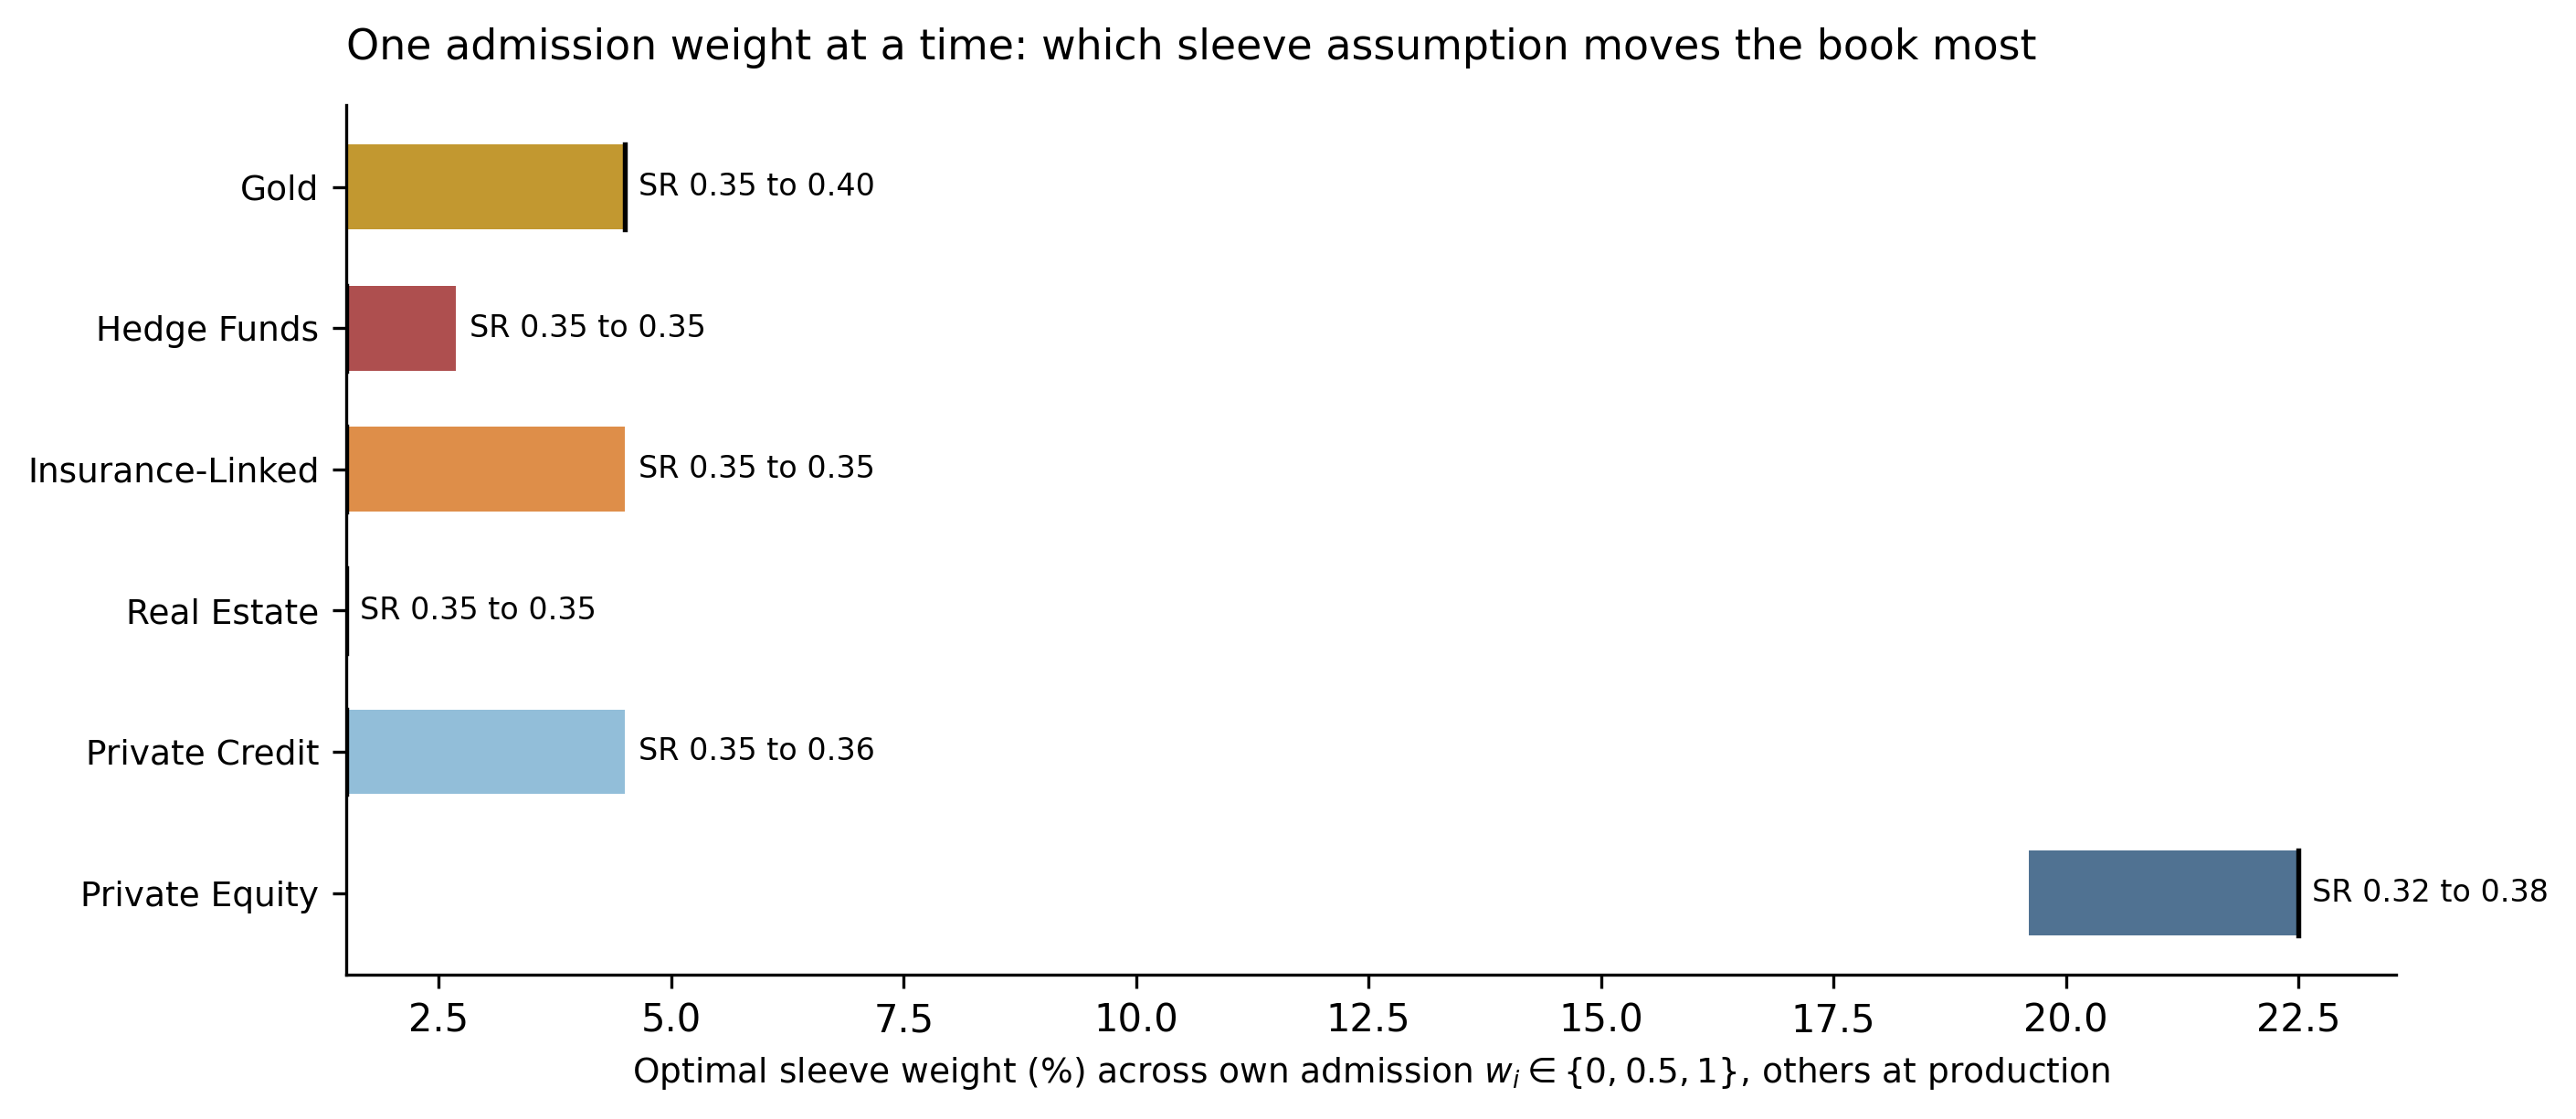
\includegraphics[width=0.8\linewidth]{figures/sleeve_tornado.PNG}
		\end{center}
		\vspace*{-1.0\baselineskip}
		{\footnotesize Notes: Balanced with Alternatives mandate, 2026-Q2 cut, USD. Each bar varies one sleeve's admission weight over $w_i \in \{0, 0.5, 1\}$ with all other sleeves at production policy, under the $\pm 50\%$ box and $1.5\%$ tracking-error constraints. Markers show the production point.}
	\end{figure}
	
	\paragraph*{The Squared-Sharpe Decomposition.}
	Exhibit~\ref{fig:sr2_decomposition} shows the four quantities cited in the main text: the frictionless factor ceiling ($0.57$), the systematic content achievable through the 18 assets ($0.24$), the raw claimed admitted-alpha content ($1.40$), and the honest content after the generalized-least-squares projection ($0.63$). The per-carrier panel uses the solo projection, under which the survived share of a single carrier's alpha equals $1 - h_i$ with $h_i$ the GLS leverage of asset $i$. The derivation, the joint-projection cross-terms, and the universe-selection application are developed in the companion paper \citep{SeppKastenholzFAJ2026}.
	
	\begin{figure}[H]
		\captionof{figure}{Claimed Versus Offered Squared Sharpe on the Production Admissions}\label{fig:sr2_decomposition}\vspace*{-0.5\baselineskip}
		\begin{center}
			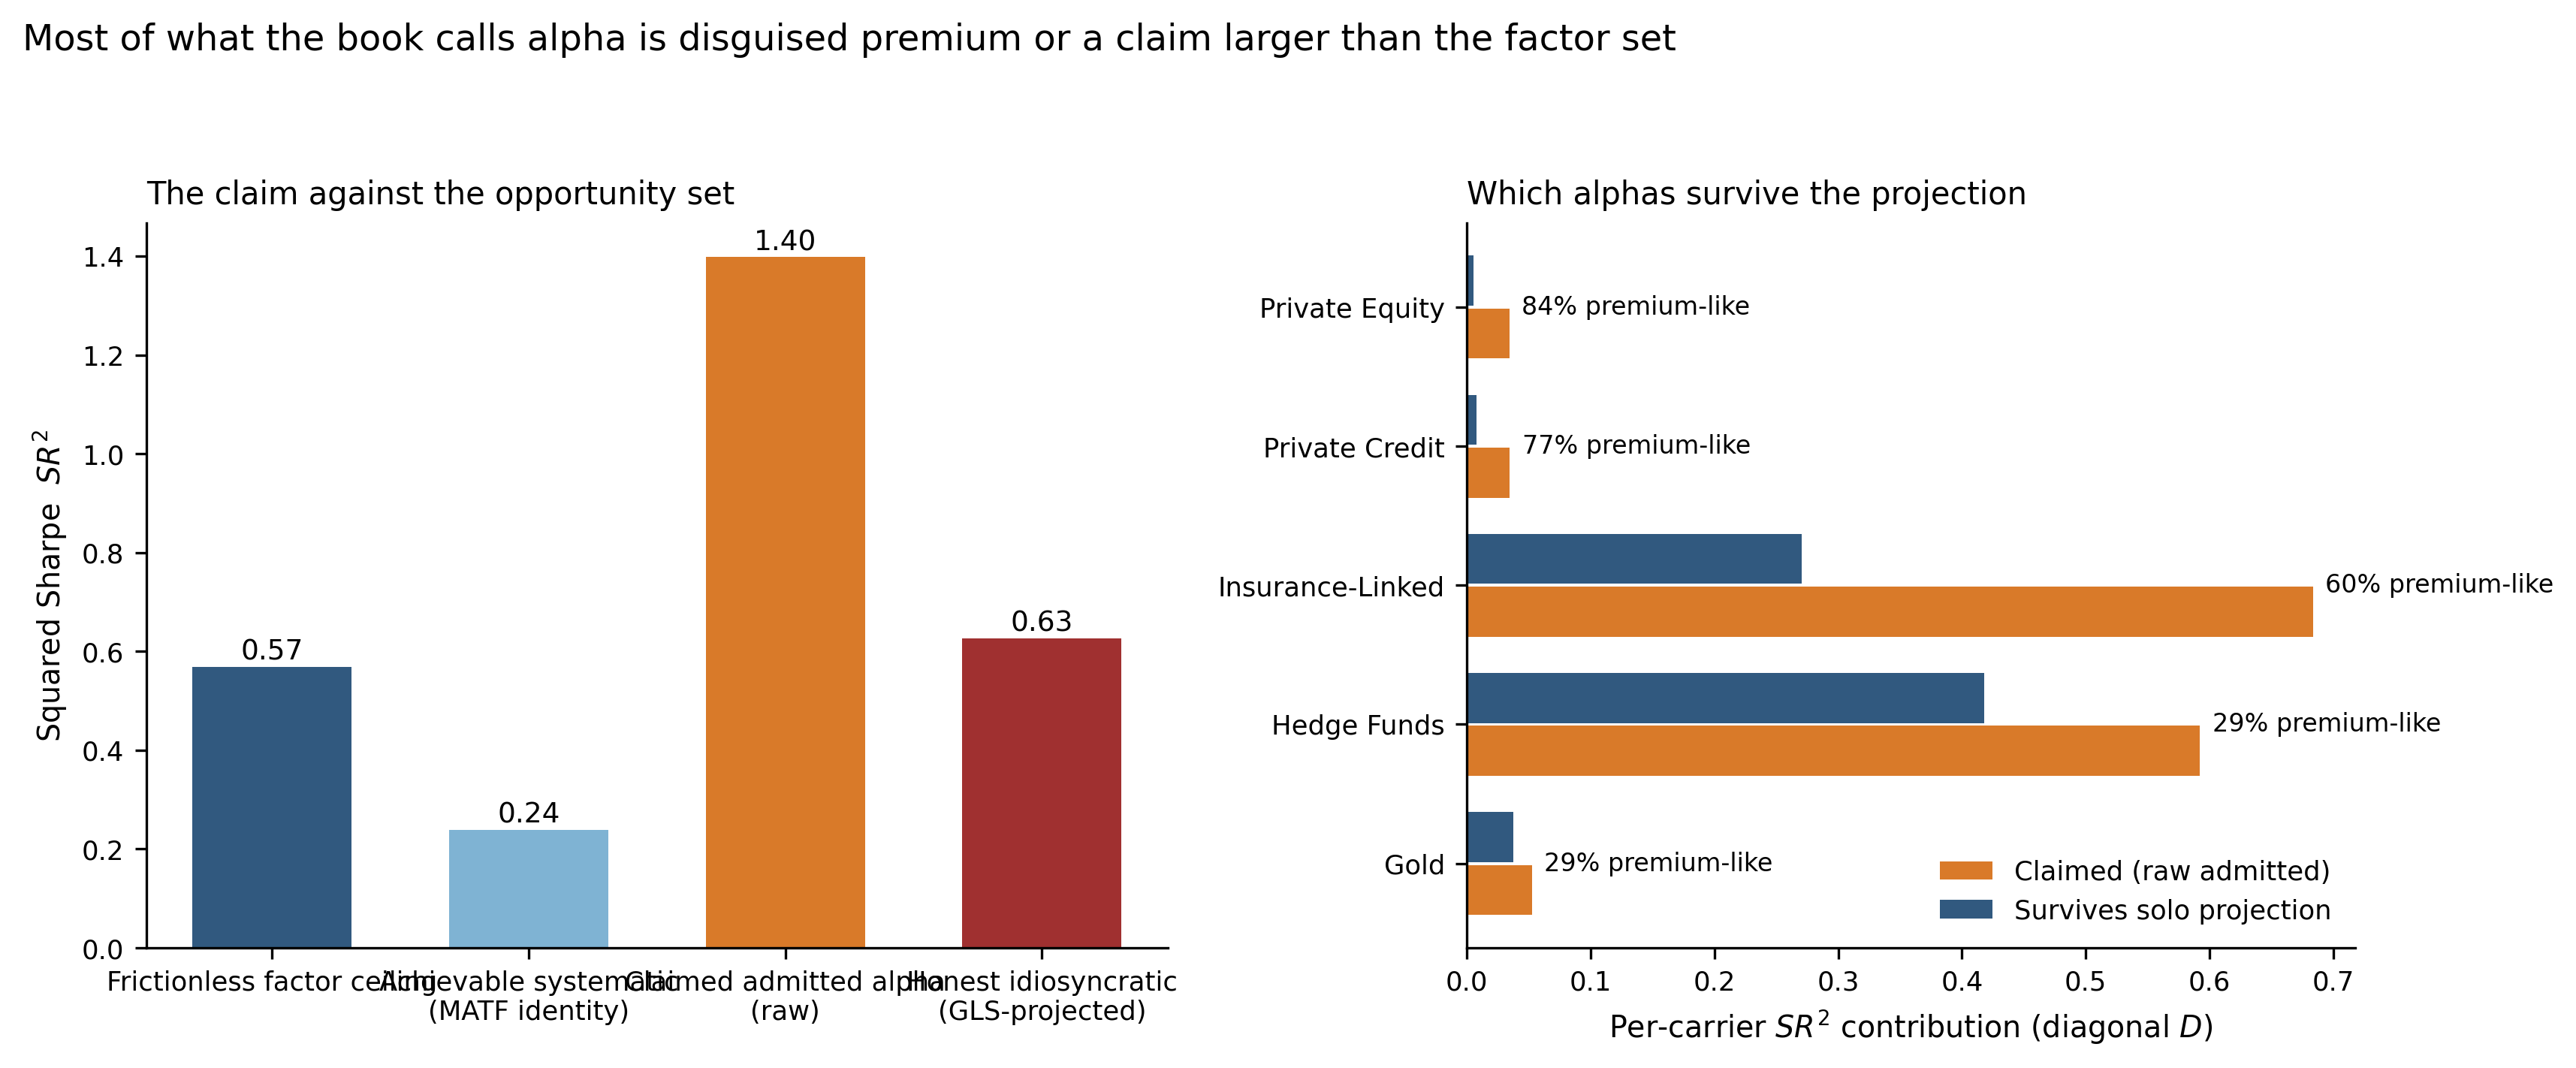
\includegraphics[width=0.95\linewidth]{figures/sr2_decomposition.PNG}
		\end{center}
		\vspace*{-1.0\baselineskip}
		{\footnotesize Notes: 2026-Q2 cut, USD. Left panel: frictionless factor ceiling $\boldsymbol\lambda^{\intercal}\Sigma_F^{-1}\boldsymbol\lambda$, achievable systematic content through the 18-asset universe, raw admitted-alpha content, and the GLS-projected honest content. Right panel: per-carrier claimed versus solo-projection-surviving content, with the premium-like share $h_i$ annotated. Method in \citet{SeppKastenholzFAJ2026}.}
	\end{figure}
	
	% ===== END appendix_e.tex =====
	
	% ===== BEGIN appendix_f.tex =====
	% Appendix F: optimization formulation + universe construction (v4 1018-1113)
	% + w/o-Alts provider frontier (frozen Q2 exhibit).
	\subsection*{Appendix F: Optimization Formulation and Universe Construction}\label{app:universe}
	
	We formulate the problem of computing the SAA weights, $\mathbf{w}^{(saa)}$, as a quadratic optimization problem. The objective function maximizes the portfolio's expected return as implied by the CMAs:
	\begin{equation}\label{eq:saa1}
		\max_{\mathbf{w}^{(saa)}} \left\{ \boldsymbol{\mu}^{\intercal}  \mathbf{w}^{(saa)}\right\} 
	\end{equation}
	where $\boldsymbol{\mu}$ is the $N$-dimensional column vector of CMA total returns, subject to the tracking error constraint of the SAA portfolio relative to the benchmark portfolio:
	\begin{equation}\label{eq:saa2}
		\left(\mathbf{w}^{(bm)} - \mathbf{w}^{(saa)}\right)^{\intercal} \Sigma^{\mathbf{Y}} \left(\mathbf{w}^{(bm)} - \mathbf{w}^{(saa)}\right)   \leq  \sigma^{2}_{\text{target}}
	\end{equation}
	where $\sigma_{\text{target}}$ is the limit of the tracking error volatility and $\Sigma^{\mathbf{Y}}$ is the covariance matrix of the TAA universe computed using Equation~\eqref{eq:cma_ii}. 
	
	
	Additional optional constraints including individual minimum and maximum bounds, the maximum and minimum limits on portfolio exposures to asset classes, portfolio turnover and group-based tracking-error limits, follow the formulation of \cite{Rosaa2026}.
	
	
	
	\paragraph*{Investable Universe and Benchmark Construction.}
	
	
	We illustrate the CMA-based SAA optimization on a simplified universe of $N=17$ assets covering three asset classes: Bonds (5 sub-assets), Equities (7 regional indexes), and Alternatives (5 sub-assets) with CMAs and factor exposures reported in Exhibit~\ref{tb:cma_snapshot}. Liquidity is excluded for simplicity. The benchmark portfolio $\mathbf{w}^{(bm)}$ serves as the neutral reference point for the optimization. Rather than defining instrument-level weights directly, we construct the benchmark through a two-level procedure: first specifying top-level asset class allocations, and then mapping these to instrument-level weights through look-through decomposition of reference indexes.
	
	We define 8 benchmark portfolios combining 4 risk profiles (Income, Low, Balanced, Growth) with two universe variants. The without-alternatives variant splits between bonds and equities at $100/0$, $70/30$, $40/60$, and $0/100$ respectively. The with-alternatives variant adds $10\%$, $20\%$, $30\%$, and $40\%$ alternatives, funded proportionally from bonds and equities:
	\begin{equation}\label{eq:illust_funding}
		W_{FI} = W_{FI}^{(0)} - q \cdot W_A, \quad W_{EQ} = W_{EQ}^{(0)} - (1-q) \cdot W_A , \quad q = \frac{W_{FI}^{(0)}}{W_{FI}^{(0)}+W_{EQ}^{(0)}} 
	\end{equation}
	where $W_{FI}^{(0)}$ and $W_{EQ}^{(0)}$ are the bond and equity allocations in the corresponding variant without alternatives. Because $q$ equals the bond share of the liquid portfolio, proportional funding preserves the ratio $W_{FI}/W_{EQ}$ regardless of the alternatives level.
	
	Exhibit~\ref{tab:benchmark_table} shows the complete benchmark construction. The top three rows display the asset class allocations for each portfolio. The ``Benchmark Weight'' column shows the within-asset-class decomposition weights $d_i^{(AC)}$ used to map from asset class allocations to instrument-level weights. Fixed income sub-asset weights are derived from the Bloomberg Multiverse index composition. Equity sub-asset weights follow the MSCI ACWI regional breakdown. Alternatives sub-asset weights are set by an indicative allocation. Each instrument-level portfolio weight is the product of the top-level asset class allocation and the corresponding decomposition weight:
	\begin{equation}\label{eq:bench_weight}
		w_i^{(bm)} = W_{AC} \times d_i^{(AC)}, \quad \sum_{i \in AC} d_i^{(AC)} = 1
	\end{equation}
	where $W_{AC} \in \{W_{FI}, W_{EQ}, W_A\}$ is the asset class allocation from Equation~\eqref{eq:illust_funding} and $d_i^{(AC)}$ is the decomposition weight of sub-asset $i$ within its benchmark. For instance, Global Government Bonds in the Low w/o Alts portfolio receives $70\% \times 54.30\% = 38.01\%$.
	
	\begin{table}[H]
		\captionof{table}{Investable Universe, Within-Class Decomposition Weights, and Benchmark Portfolio Weights}\label{tab:benchmark_table}\vspace*{-1.0\baselineskip}
		\begin{center}
			\pendingexhibit[width=1.0\linewidth]{figures/benchmark_table.png}\vspace*{-1.0\baselineskip}
		\end{center}
		\small
		NOTE: The top three rows show asset class allocations. The remaining rows show instrument-level weights computed as the product of the asset class allocation and the decomposition weight.
	\end{table}
	
	
	
	For each of the eight benchmark portfolios, we solve the optimization problem in Equations~(\ref{eq:saa1})--(\ref{eq:saa2}) with the following constraint specification:
	
	\textbf{1) Tracking error constraint:} $\sigma_{\text{target}} = 1.5\%$ annualized, applied to the total portfolio relative to the benchmark using Equation~\eqref{eq:saa2}.
	
	\textbf{2) Individual asset weight bounds:} For each asset $n$, the individual minimum and maximum bounds are set symmetrically around the benchmark weight with a band parameter $b = 50\%$:
	\begin{equation}\label{eq:illust_bounds}
		l_n = (1 - b) \cdot w_n^{(bm)} , \quad u_n = (1 + b) \cdot w_n^{(bm)} 
	\end{equation}
	
	This ensures that the optimizer can at most halve or increase by 50\% any given benchmark position, allowing meaningful active tilts.
	
	\textbf{3) No group constraints or turnover constraints} are imposed in this illustration.
	
	
	
	The constraint specification is deliberately parsimonious: the tracking-error budget controls the magnitude of active risk while the proportional bounds limit concentration. Production deployments add group-level constraints (e.g., maximum equity overweight of $15\%$) and turnover limits.
	
	
	Exhibit~\ref{fig:illust_frontier} plots the expected return versus volatility for all eight benchmark portfolios and the optimized portfolios. The four mandates frontiers trace out the risk-return profiles available to a multi-asset investor under the MATF-CMA framework.
	
	\begin{table}[H]
		\captionof{table}{Efficient Frontier for Benchmark and Optimized Portfolios Across Four Risk Profiles (Income, Low, Balanced, Growth)}\label{fig:illust_frontier}\vspace*{-1.5\baselineskip}
		\begin{center}
			\pendingexhibit[width=0.80\textwidth]{figures/efficient_frontier.PNG}\vspace*{-1.5\baselineskip}
		\end{center}
		\small
		NOTE: Notation: w/o Alts - benchmark is benchmark without alternatives, with Alts - benchmark is benchmark with alternatives, w/o Alts - portfolio is optimized portfolio without alternatives, and with Alts - portfolio is optimized portfolio with alternatives. USD reference currency. Tracking error constraint: 1.5\%, weight band: $\pm 50\%$.
	\end{table}
	
	
	Across all eight portfolios, the optimization achieves a higher expected return than the corresponding benchmark within the 1.5\% tracking error budget. The Balanced portfolio without alternatives improves from 5.6\% to 6.0\%, and with alternatives from 6.4\% to 7.1\%. In both cases, the full tracking error budget is consumed, directing active risk toward assets with the highest expected return relative to their risk contribution.
	
	The optimizer systematically tilts toward assets with higher CMAs within the tracking error and bound constraints. In the fixed income sleeve, the optimizer overweights HY and EM HC Bonds (CMAs of approximately $5\%$) at the expense of Government Bonds (CMA of $4.4\%$). In the alternatives sleeve, the optimizer overweights Private Equity (CMA of $10.3\%$) and Real Assets ($6.1\%$) relative to Hedge Funds ($4.2\%$). These tilts are consistent with the factor risk premia embedded in the CMAs: the Equity factor premium (approximately $2.4\%$) and the Credit factor premium reward assets with higher loadings on these factors.
	
	We see that portfolios with alternatives consistently achieve higher Sharpe ratios than their counterparts without alternatives, both at the benchmark level and after optimization. The alternatives allocation introduces exposure to the Inflation, Commodities, and Private Equity factors, which are largely orthogonal to the Equity and Rates factors that dominate traditional portfolios.
	
	
	Exhibit~\ref{tab:factor_exposures} reports the MATF factor exposures and the corresponding percentage risk contributions for the eight optimized portfolios. The Equity factor dominates the risk decomposition across all profiles: even the Income w/o Alts portfolio, which holds no equities, has a 22\% Equity risk contribution arising from the credit and EM bond exposures. As the equity allocation increases, the Equity factor's risk share rises to 70-85\%. The introduction of alternatives partially mitigates this concentration: the Growth with Alts portfolio reduces the Equity risk share from 86\% to 77\% by introducing exposure to alternatives with factors risk largely orthogonal to the Equity-Rates axis. Nevertheless, the Equity factor remains the dominant risk driver in all eight portfolios, confirming that multi-asset diversification at the asset class level does not eliminate factor concentration.\vspace*{-0.5\baselineskip}
	
	\begin{table}[H]
		\captionof{table}{MATF Portfolio Beta Exposures and Percentage Risk Contributions}\label{tab:factor_exposures}\vspace*{-1.0\baselineskip}
		\begin{center}
			\pendingexhibit[width=0.75\textwidth]{figures/factor_exposures.png}\vspace*{-1.0\baselineskip}\vspace*{-1.0\baselineskip}
		\end{center}
		\small
	\end{table}
	
	
	
	
	\sectionfont{\MakeUppercase}
	
	\paragraph*{The w/o-Alternatives Provider Frontier.}
	Exhibit~\ref{fig:provider_frontier_wo} repeats the provider comparison of Section ``Decision One: The Provider Choice'' on the four mandates without alternatives. The bond block carries the rotation in this family: the Global Government weight runs from $10.9\%$ to $15.8\%$ across providers on the Balanced mandate, while the equity dispersion mirrors the with-Alternatives family.
	
	\begin{figure}[H]
		\captionof{figure}{Provider Frontiers on the Common Risk Model: w/o-Alternatives Mandate Family}\label{fig:provider_frontier_wo}\vspace*{-0.5\baselineskip}
		\begin{center}
			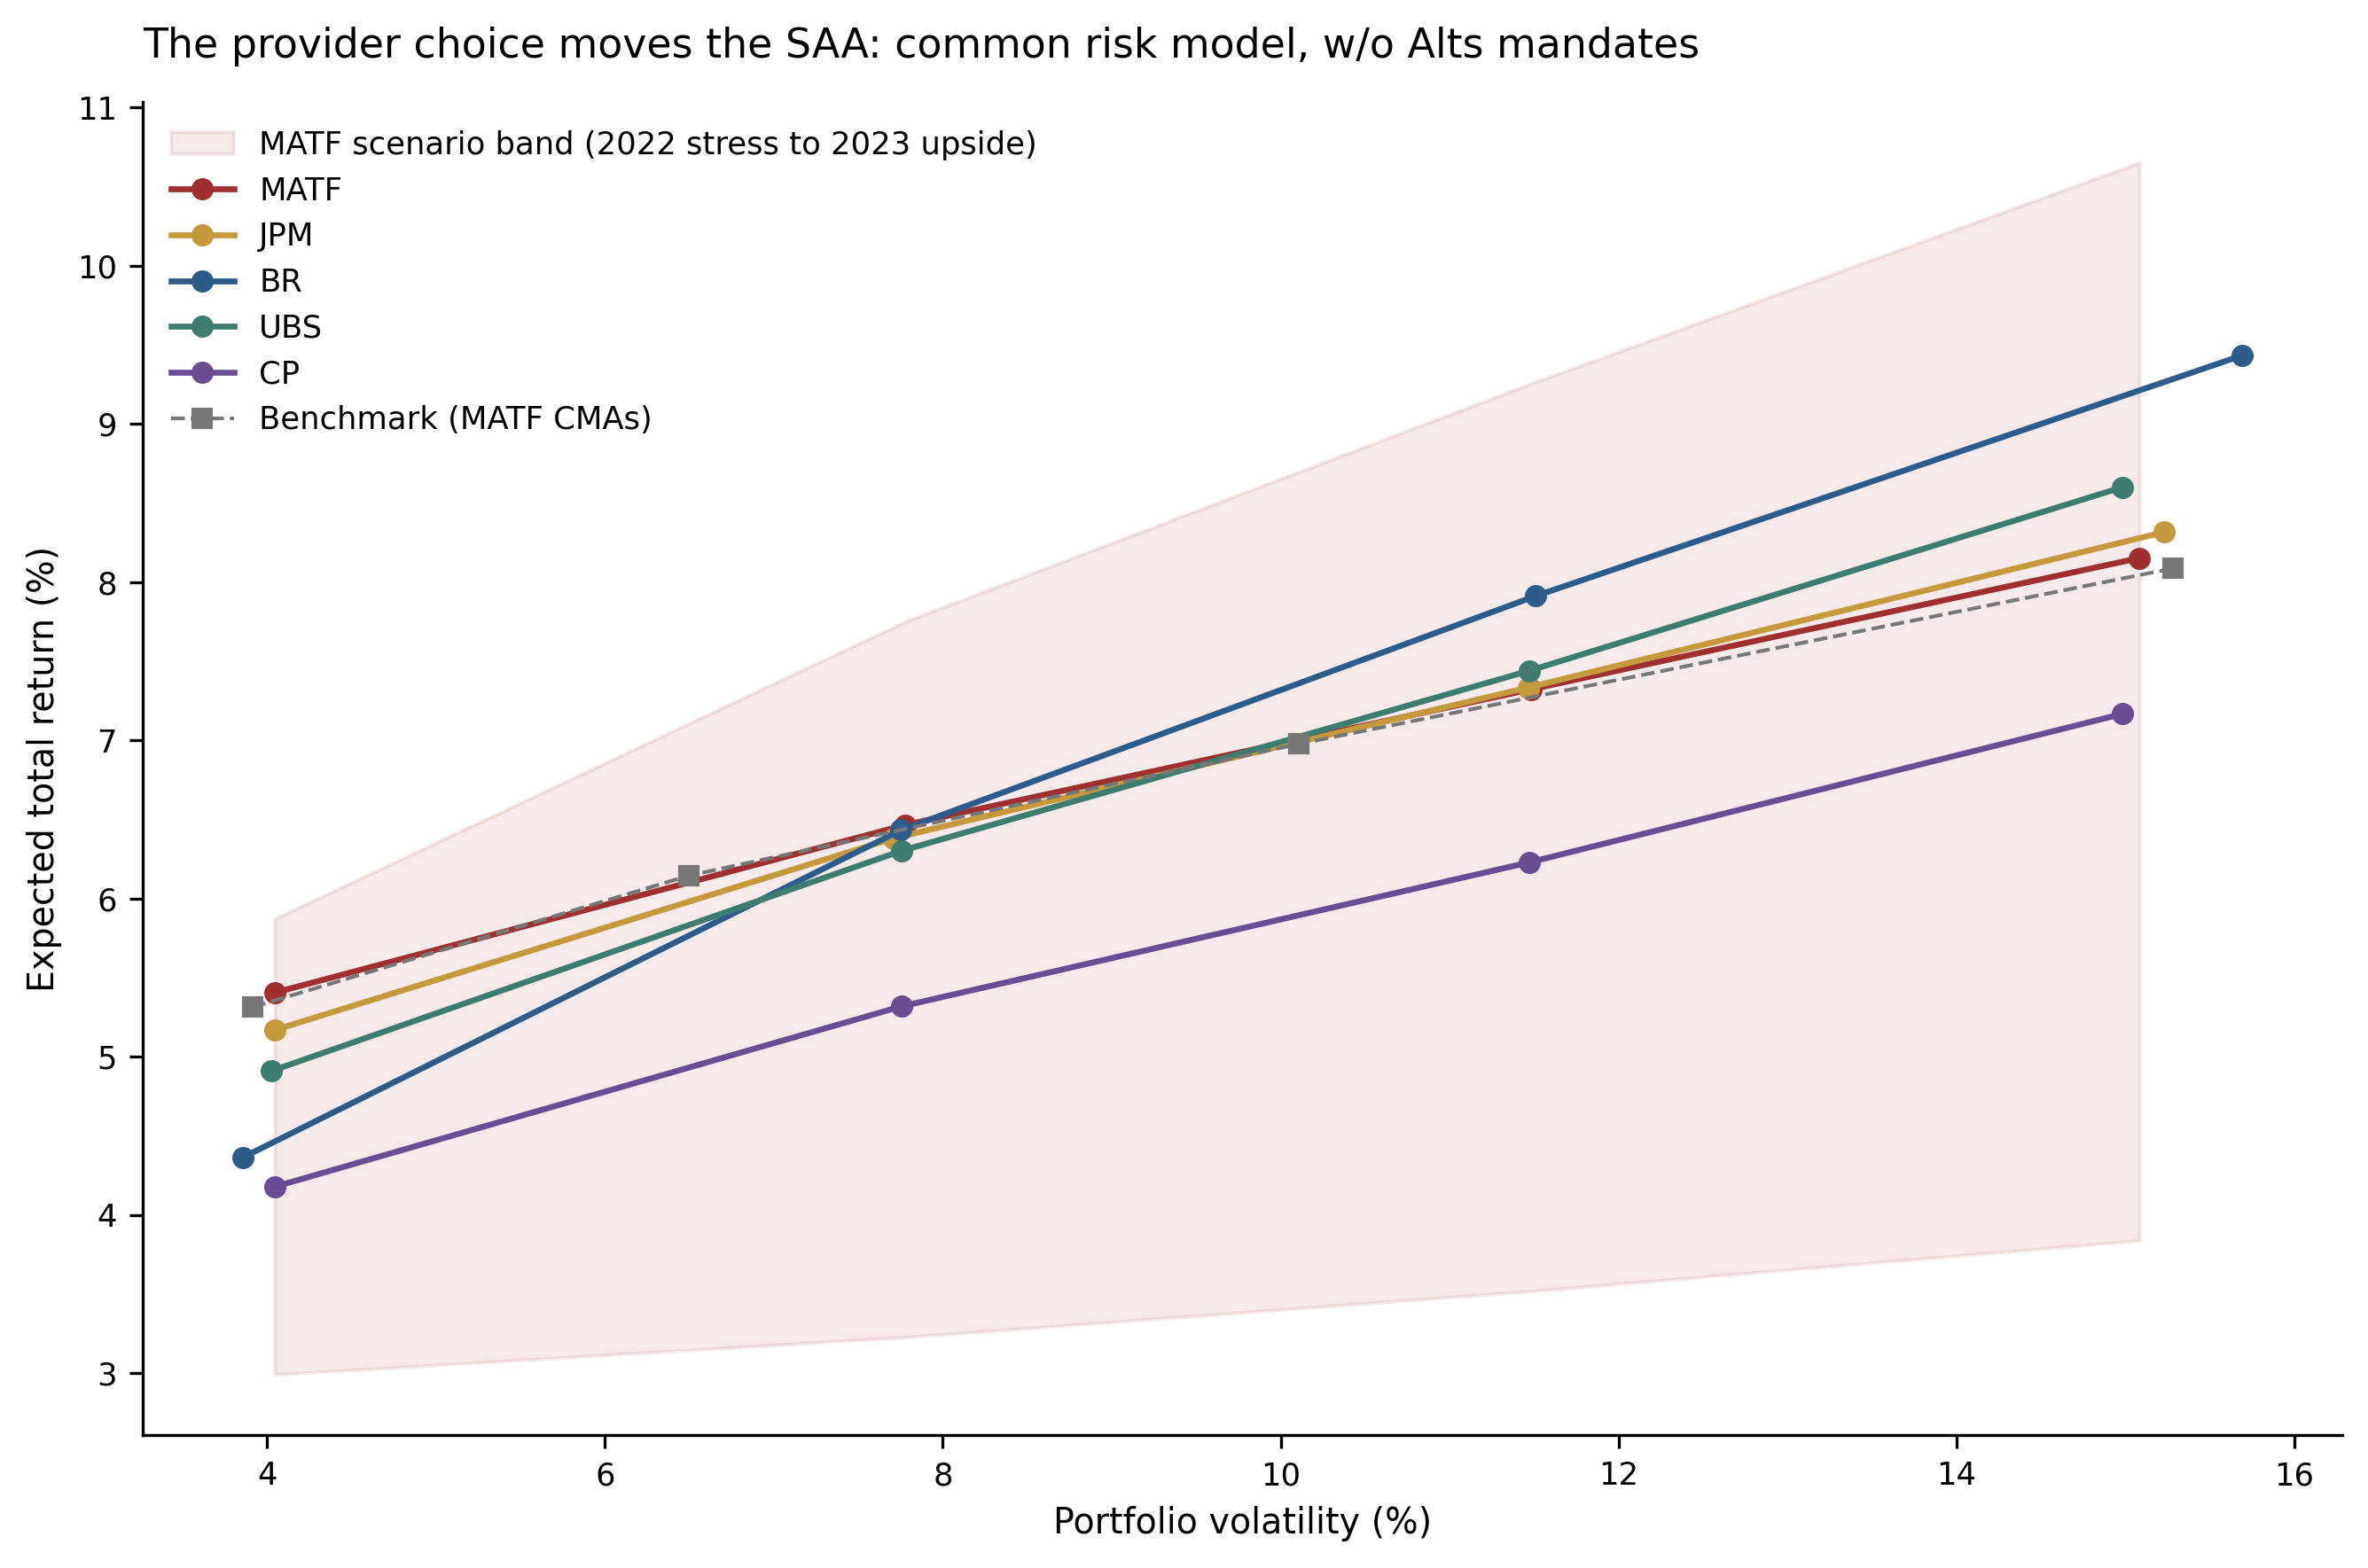
\includegraphics[width=0.8\linewidth]{figures/provider_frontier_wo_alts.PNG}
		\end{center}
		\vspace*{-1.0\baselineskip}
		{\footnotesize Notes: as Exhibit~\ref{fig:provider_frontier}, for the Income, Low, Balanced, and Growth mandates without alternatives, 2026-Q2 cut, USD.}
	\end{figure}
	
	% ===== END appendix_f.tex =====
	
	% ===== BEGIN bibliography_r2.tex =====
	% v4 bibliography (1410-1498) + R2 additions.
	\begin{thebibliography}{}
		
		\bibitem[\protect\citeauthoryear{Adrian, Crump, and Moench}{2013}]{ACM2013}
		Adrian, T., R.K. Crump, and E. Moench. 2013. ``Pricing the Term Structure with Linear Regressions.'' \textit{Journal of Financial Economics} 110 (1): 110--138.
		
		\bibitem[\protect\citeauthoryear{Ang et al.}{2018}]{Ang2018}
		Ang, A., B. Chen, W.N. Goetzmann, and L. Phalippou. 2018. ``Estimating Private Equity Returns from Limited Partner Cash Flows.'' \textit{Journal of Finance} 73 (4): 1751--1783.
		
		\bibitem[\protect\citeauthoryear{AQR}{2020}]{AQR2020}
		AQR Portfolio Solutions Group. 2020. ``Was That Intentional? Ways to Improve Your Active Risk.'' \textit{Alternative Thinking}, 3Q 2020.
		
		\bibitem[\protect\citeauthoryear{Black and Litterman}{1992}]{BlackLitterman1992}
		Black, F. and R. Litterman. 1992. ``Global Portfolio Optimization.'' \textit{Financial Analysts Journal} 48 (5): 28--43.
		
		\bibitem[\protect\citeauthoryear{Brinson, Hood, and Beebower}{1986}]{BHB1986}
		Brinson, G.P., L.R. Hood, and G.L. Beebower. 1986. ``Determinants of Portfolio Performance.'' \textit{Financial Analysts Journal} 42 (4): 39--44.
		
		\bibitem[\protect\citeauthoryear{Campbell and Shiller}{1988}]{CampbellShiller1988}
		Campbell, J.Y. and R.J. Shiller. 1988. ``Stock Prices, Earnings, and Expected Dividends.'' \textit{Journal of Finance} 43 (3): 661--676.
		
		\bibitem[\protect\citeauthoryear{Ceria, Sivaramakrishnan, and Stubbs}{2013}]{CeriaStubbsAlpha2013}
		Ceria, S., K. Sivaramakrishnan, and R.A. Stubbs. 2013. ``Alpha Construction in a Consistent Investment Process.'' Axioma Research Paper No.~045.
		
		\bibitem[\protect\citeauthoryear{Chopra and Ziemba}{1993}]{ChopraZiemba1993}
		Chopra, V.K. and W.T. Ziemba. 1993. ``The Effect of Errors in Means, Variances, and Covariances on Optimal Portfolio Choice.'' \textit{Journal of Portfolio Management} 19 (2): 6--11.
		
		\bibitem[\protect\citeauthoryear{Cochrane}{2005}]{Cochrane2005}
		Cochrane, J.H. 2005. \textit{Asset Pricing}. Princeton: Princeton University Press.
		
		\bibitem[\protect\citeauthoryear{DeMiguel, Garlappi, and Uppal}{2009}]{DeMiguelGarlappiUppal2009}
		DeMiguel, V., L. Garlappi, and R. Uppal. 2009. ``Optimal Versus Naive Diversification: How Inefficient is the 1/N Portfolio Strategy?'' \textit{Review of Financial Studies} 22 (5): 1915--1953.
		
		\bibitem[\protect\citeauthoryear{Elkamhi, Lee, and Salerno}{2021}]{ElkamhiLeeSalerno2021}
		Elkamhi, R., J.S.H. Lee, and M. Salerno. 2021. ``Factor Investing Using Capital Market Assumptions.'' \textit{Journal of Portfolio Management} 48 (2): 119--143.
		
		\bibitem[\protect\citeauthoryear{Gon\c{c}alves}{2025}]{Goncalves2025}
		Gon\c{c}alves, A.S. 2025. ``What Moves Equity Markets? A Term Structure Decomposition for Stock Returns.'' Kenan Institute Working Paper.
		
		\bibitem[\protect\citeauthoryear{Greenberg, Babu, and Ang}{2016}]{GreenbergBabuAng2016}
		Greenberg, D., A. Babu, and A. Ang. 2016. ``Factors to Assets: Mapping Factor Exposures to Asset Allocations.'' \textit{Journal of Portfolio Management} 42 (5): 18--27.
		
		\bibitem[\protect\citeauthoryear{Grinold and Kroner}{2002}]{GrinoldKroner2002}
		Grinold, R.C. and K.F. Kroner. 2002. ``The Equity Risk Premium.'' \textit{Investment Insights} 5 (3): 7--33.
		
		\bibitem[\protect\citeauthoryear{Haghani and White}{2024}]{HaghaniWhite2024}
		Haghani, V. and J. White. 2024. ``Introducing P-CAPE.'' Elm Wealth Research Note.
		
		\bibitem[\protect\citeauthoryear{Ilmanen}{2011}]{Ilmanen2011}
		Ilmanen, A. 2011. \textit{Expected Returns: An Investor's Guide to Harvesting Market Rewards}. Chichester: John Wiley \& Sons.
		
		\bibitem[\protect\citeauthoryear{Lemp\'eri\`ere et al.}{2017}]{Lemperiere2017}
		Lemp\'eri\`ere, Y., C. Deremble, T.-T. Nguyen, P. Seager, M. Potters, and J.-P. Bouchaud. 2017. ``Risk Premia: Asymmetric Tail Risks and Excess Returns.'' \textit{Quantitative Finance} 17 (1): 1--14.
		
		\bibitem[\protect\citeauthoryear{Lo}{2002}]{Lo2002}
		Lo, A.~W. 2002. ``The Statistics of Sharpe Ratios.'' \textit{Financial Analysts Journal} 58 (4): 36--52.
		
		\bibitem[\protect\citeauthoryear{Lustig, Roussanov, and Verdelhan}{2011}]{LustigRV2011}
		Lustig, H., N. Roussanov, and A. Verdelhan. 2011. ``Common Risk Factors in Currency Markets.'' \textit{Review of Financial Studies} 24 (11): 3731--3777.
		
		\bibitem[\protect\citeauthoryear{Morris}{2026}]{Morris2026}
		Morris, S. 2026. ``Interest Rate Volatility as a Systematic Risk Factor.'' Nomura Quantitative Research.
		
		
		
		\bibitem[\protect\citeauthoryear{Park and Casella}{2008}]{ParkCasella2008}
		Park, T. and G. Casella. 2008. ``The Bayesian Lasso.'' \textit{Journal of the American Statistical Association} 103 (482): 681--686.
		
		\bibitem[\protect\citeauthoryear{Politis and Romano}{1994}]{PolitisRomano1994}
		Politis, D.N. and J.P. Romano. 1994. ``The Stationary Bootstrap.'' \textit{Journal of the American Statistical Association} 89 (428): 1303--1313.
		
		\bibitem[\protect\citeauthoryear{Roncalli, Abou~Rjaily, and Xu}{2024}]{RoncalliXu2024}
		Abou~Rjaily, N., T. Roncalli, and J. Xu. 2024. ``Risk Factor, Risk Premium
		and Black--Litterman Model.'' SSRN Working Paper No.~4976695.
		
		\bibitem[\protect\citeauthoryear{Ross}{1976}]{Ross1976}
		Ross, S.A. 1976. ``The Arbitrage Theory of Capital Asset Pricing.'' \textit{Journal of Economic Theory} 13 (3): 341--360.
		
		\bibitem[\protect\citeauthoryear{Saxena and Stubbs}{2013}]{SaxenaStubbsAAF2013}
		Saxena, A. and R.A. Stubbs. 2013. ``The Alpha Alignment Factor: A Solution to the Underestimation of Risk for Optimized Active Portfolios.'' \textit{The Journal of Risk} 15 (3): 3--37.
		
		\bibitem[\protect\citeauthoryear{Sepp}{2026}]{MatfCmaCode2026}
		Sepp, A. 2026. ``Replication Code for Capital Market Assumptions Using Multi-Asset Tradable Factors: The MATF-CMA Framework.'' \textit{GitHub}. \url{https://github.com/ArturSepp/OptimalPortfolios/tree/master/paper_code/matf_cma_jpm_2026}.
		
		
		\bibitem[\protect\citeauthoryear{Sepp, Ossa, and Kastenholz}{2026}]{Rosaa2026}
		Sepp, A., I. Ossa, and M.A. Kastenholz. 2026. ``Robust Optimization of Strategic and Tactical Asset Allocation for Multi-Asset Portfolios.'' \textit{Journal of Portfolio Management} 52 (4): 86--120.
		
		
		
		\bibitem[\protect\citeauthoryear{Horizon Actuarial Services}{2025}]{HorizonSurvey2025}
		Horizon Actuarial Services, LLC. 2025. ``Survey of Capital Market Assumptions: 2025 Edition.'' August 2025.
		
		\bibitem[\protect\citeauthoryear{Malkiel and Saha}{2005}]{MalkielSaha2005}
		Malkiel, B.G. and A. Saha. 2005. ``Hedge Funds: Risk and Return.'' \textit{Financial Analysts Journal} 61 (6): 80--88. [TODO: confirm entry]
		
		\bibitem[\protect\citeauthoryear{Sepp and Kastenholz}{2026}]{SeppKastenholzFAJ2026}
		Sepp, A. and M.A. Kastenholz. 2026. ``Achievable Sharpe and Universe Selection: A Closed-Form Factor Decomposition.'' Under review at the \textit{Financial Analysts Journal}.
		
	\end{thebibliography}
	% ===== END bibliography_r2.tex =====
	
\end{document}